% !TeX program = pdflatex

\documentclass[]{article}

% Packages
\usepackage{graphicx}
\usepackage{biblatex}
\usepackage{subfiles}
\usepackage{standalone}
\usepackage{import}
\usepackage{amsmath}
\usepackage{amssymb} % For math symbol E (expected)
\usepackage{datetime} % Title page current date
\usepackage{hyperref} % For now I'm just seeing the green bounding boxes around citations
\usepackage{url} % For URL references
\usepackage[symbol]{footmisc} % For footnotes symbols

% For code listings
\usepackage{listings}
\usepackage{color}
\usepackage[x11names,table]{xcolor}

\definecolor{codebg}{rgb}{0.96, 0.96, 0.96}
\definecolor{codeborder}{rgb}{0.78, 0.78, 0.78}
\definecolor{keywordcolor}{rgb}{0, 0, 1}
\definecolor{stringcolor}{rgb}{0.64, 0.08, 0.08}
\definecolor{commentcolor}{rgb}{0, 0.5, 0}
\definecolor{identifiercolor}{rgb}{0, 0, 0}
\definecolor{numbercolor}{rgb}{0.5, 0, 0.5}

% Define custom style for Python code
\lstdefinestyle{mypython}{
    backgroundcolor=\color{codebg},
    frame=single,
    rulecolor=\color{codeborder},
    basicstyle=\ttfamily\small,
    keywordstyle=\color{keywordcolor}\bfseries,
    stringstyle=\color{stringcolor},
    commentstyle=\color{commentcolor}\itshape,
    identifierstyle=\color{identifiercolor},
    numberstyle=\color{numbercolor},
    numbers=left,
    numbersep=5pt,
    showspaces=false,
    showstringspaces=false,
    language=Python,
}

% Apply the custom style to Python code
\lstset{style=mypython}


% For figures
\usepackage{tikz}
\usetikzlibrary{shapes,arrows.meta,positioning,automata,calc,fit,matrix}

% For timeline figures
\usepackage{geometry} 

% For plots
\usepackage{pgfplots}
\pgfplotsset{compat=newest}

% References
\newpage
\addbibresource{references.bib}

% Define general colors for use
\definecolor{lightblue}{rgb}{0.678, 0.847, 0.902}
\definecolor{lightgreen}{rgb}{0.678, 0.902, 0.847}
\definecolor{lightred}{rgb}{0.902, 0.678, 0.847}
\definecolor{lightgray}{rgb}{0.902, 0.902, 0.902}

\definecolor{darkgray}{rgb}{0.502, 0.502, 0.502}


\usepackage{tocbibind} % Automatically includes bibliography in the ToC
\usepackage{empheq} % For boxing equations
\usepackage{sidecap} % Include this in the preamble
\usepackage{subcaption} % For subfigures
\usepackage{tikz-cd} % For equation down arrows
\usepackage{array} % For tabular column width

\begin{document}

% Cover (Title page)
\begin{titlepage}
    \begin{center}
        \vspace*{1cm}
        
        
\includegraphics[width=0.2\textwidth]{images/ou_logo.png}\\
        The Open University of Israel\\
        Department of Mathematics and Computer Science
        
        \vspace{2cm}
        
        {\Large \textbf{An Overview of Deep Learning Techniques for Image and Video Generation}}
        \vspace{1.5cm}
        
        Final paper submitted as partial fulfillment of the requirements\\towards an M.Sc. degree in Computer Science\\
        The Open University of Israel\\
        Department of Mathematics and Computer Science
        
        \vspace{1cm}
        
        By \\
        \textbf{Shlomi Domnenko}
        
        \vspace{1cm}
        
        Prepared under the supervision of \textbf{Dr. Mireille Avigal}
        
        \vfill
        
        \textbf{May 2025}
    \end{center}
\end{titlepage}

% Table of Contents (ToC)
\tableofcontents
\newpage

% Abstract
\section{Abstract}

% TODO: Need to add more examples of good models, in particular video generation.

This research paper examines recent progress in image and video synthesis using machine learning (ML). While image synthesis has reached a considerable degree of maturity with the development of sophisticated deep learning models, video synthesis continues to present significant research challenges.

Deep generative models, particularly prominent models like DALL-E \cite{dalle}, Sora \cite{sora_website}, Midjourney \cite{midjourney-website}, have gained significant attention due to their ability to produce high-resolution and creative images and videos. In this paper we will focus on 3 image synthesis models and 3 video synthesis models that had a significant contribution to the advancement of the domain. In image synthesis will focus on VQ-GAN \cite{vqgan}, Stable Diffusion \cite{stable_diffusion} and Imagen \cite{imagen}. In video synthesis we will focus on Video-LDM \cite{video_ldm}, Stable Video Diffusion (SVD) \cite{stable_video_diffusion} and Make-a-Video \cite{make_a_video}.

This paper surveys the recent advancements in ML techniques for image and video generation. We explore the fundamental concepts underlying these techniques, focusing on how they learn to create realistic and compelling visual content. We place particular emphasis on the video generation domain, recognizing its immense potential and future applications.

% TODO: Add examples of models to "Diffusion Models", add references to mentioned models
The paper delves into various image generation models, including Variational Autoencoders (VAEs) \cite{vae}, Generative Adversarial Networks (GANs) \cite{gan}, and Diffusion Models (DMs) \cite{dpms}. We discuss their working principles, strengths, and limitations. Additionally, we explore the use of conditioning to control the output, temporal and spatial cohesion in video synthesis, dataset preparation and learning optimization. Finally, we explore video synthesis techniques that build upon these image generation models, highlighting their unique challenges and interesting points.
\newpage

% Introduction
\section{Introduction}

The field of image and video synthesis is large and continuously expanding. While image generation has come a long way, recent advancements in video synthesis emerged recently, highlighted by the significant breakthrough of OpenAI's Sora model \cite{sora_website}. A solid foundation in image synthesis techniques is essential to fully comprehend the methodologies and techniques involved in video synthesis.

In this work we will review two main models that are used as a basis in image and video generation models: Generative Adversarial Networks (GANs) \cite{gan} \ref{sec:gan} and Diffusion Probabilistic Models (DPMs) \cite{diffusion_models} \cite{ddpm} \ref{sec:ddpm}.

In generative models we are given a set of data points (e.g. images) and our goal is to create a new sample (new image) from this dataset. That is, we don't want to randomly select an image from the dataset, but rather we want to create a new image that does not appear in the dataset, but is similar to it. The key word is "similar" - mathematically speaking, we are talking about predicting the probability function of the dataset. That is, the model needs to learn the underlying distribution of the dataset and create new samples that represent the same distribution. Generative models provide an efficient method for analyzing and understanding unlabeled data in unsupervised learning.

Advanced image synthesis models like DALL-E \cite{dalle} and Stable Diffusion \cite{stable_diffusion} represent a significant milestone in the field. While recent models may not offer groundbreaking advancements, the landscape of long video synthesis remains relatively unexplored. Video synthesis presents unique challenges compared to image synthesis, primarily due to the introduction of the temporal dimension.

New models for generating images and videos are developed by building upon existing models, enhancing them through innovative techniques and adjustments. In this work we explore the VQ-GAN model \cite{vqgan} \ref{vqgan} which combines the GAN model \cite{gan} \ref{sec:gan} with the VQ-VAE model \cite{vqvae} \ref{vqvae} and the Transformer model \cite{transformer} (appendix \ref{appendix:transformers}) together. Notably, VQ-GAN generates images based on textual descriptions, converting text inputs into visual outputs that reflect the text's description. The VQ-VAE model, derived from the VAE model \cite{vae} \ref{sec:vae} and employing vector quantization technique \cite{vqvae} \ref{sec:vq}, is itself an advancement of the Autoencoder model \cite{autoencoder} \ref{sec:vae}. In short, understanding these models and their inner workings requires prior familiarity with their foundations and previous works.

Another example is the Variational Autoencoder (VAE) \cite{vae} \ref{sec:vae} model, which is used as a basis in VQ-VAE model. 

\begin{figure}[H]
    \centering
    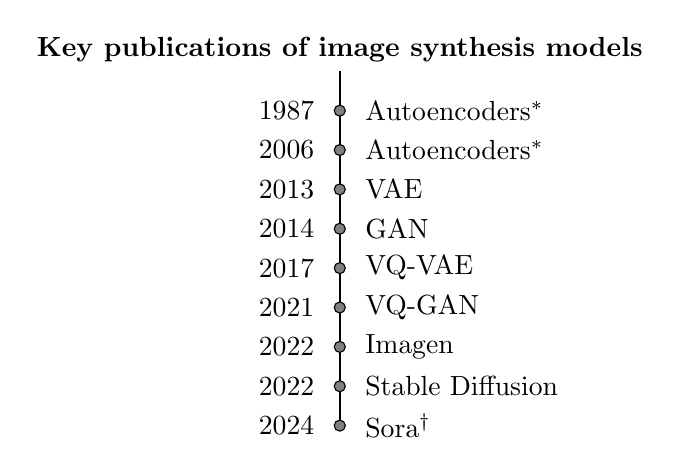
\begin{tikzpicture}
        \def\step{0.5} % step size for vertical spacing
        \def\numtimeline{9} % Number of events in the timeline

        % Define timeline line
        \draw[thick, color=black] (0,0) -- (0,-\numtimeline*\step);

        % Define timeline events with adjusted positions
        \foreach \i/\year/\text in 
        {
            1/1987/Autoencoders$^*$, 
            2/2006/Autoencoders$^*$, 
            3/2013/VAE, 
            4/2014/GAN, 
            5/2017/VQ-VAE,
            6/2021/VQ-GAN,
            7/2022/Imagen,
            8/2022/Stable Diffusion,
            9/2024/Sora$^\dag$
        } {
        \draw[fill=darkgray] (0,-\i*\step) circle (2pt);
        \node[anchor=east] at (-0.2,-\i*\step) {\year};
        \node[anchor=west] at (0.2,-\i*\step) {\text};
        }

        % Define timeline title
        \node[anchor=south] at (0,0) {\textbf{Key publications of image synthesis models}};
    \end{tikzpicture}
    \caption{Chronology of key image generation models publications $^*$The earliest mention of autoencoders appears in an 1986 publication \cite{autoencoder_original_paper_1986}, however the model was not widely used until 2006 when Hinton published a paper that uses autoencoders for dimensionality reduction \cite{autoencoder_2006_paper} which sparked interest in the model again.$^\dag$Although Sora \cite{sora_website} is not specifically an image generation model, it is considered a significant advancement in video synthesis field, which largely relies on image generation.}
    \label{fig:timeline}
  \end{figure}

\subsection{Mathematical Formulation of Generative Models}
Mathematically speaking, let $x$ be a random variable representing a single data point (e.g. an image) of a dataset ${x_1,x_2,...,x_n}$. And let $p(x)$ denote the true probability density function (PDF) of the dataset. Then our objective (as in generative modeling) is to learn a function $q(x;\theta)$ that approximates the true data distribution $p(x)$ (where $\theta$ is the model's parameters). The goal is to estimate $p(x)$ such that new samples $\hat{x} \in p(x)$ drawn from this distribution resemble the dataset.

Most of the time, it is infeasible to calculate directly $p(x)$ because computing the exact probability density for high-dimensional data is computationally expensive and often requires integrating over a large number of variables. This complexity leads to intractable calculations, making it difficult to directly model $p(x)$. Instead, we use various techniques to approximate it, and we denote it as: $q(x;\theta) \sim p(x)$.

\subsection{Approximating the Data Distribution}

In order to approximate $p(x)$ we can use a generative model, where the training objective is to learn the parameters $\theta$ of the model. The success or failure of the model to correctly approximate the dataset distribution can be evaluated using different loss functions, such as maximizing likelihood functions (Appendix \ref{appendix:likelihood_function}), minimizing Kullback-Leibler (KL) divergence, or using adversarial training loss (in the case of GANs).

\subsection{Sampling}

Once trained, the generative model can be used to generate new samples $\hat{x} \sim q(x;\theta)$. Sampling data point $\hat{x}$ will be consistent with the patterns and characteristics of the original dataset, as the model has learned to approximate the true data distribution. Each model will have different strategies to sample. For example, in GANs a random noise vector is sampled from a normal distribution and passed through the generator to generate a new sample, and in VQ-GAN a transformer is used to generate latent codes that are then passed through the decoder to generate an image.

\subsection{Evaluation metrics}

Evaluation of the trained model is done using metrics such as sample quality, diversity (variety in generated samples), and coverage (how well the model covers the data distribution). As we will find later, one of the main problems of the GAN model is called 'mode collapse' \ref{gan_mode_collapse} which causes instability of the model during training, which is manifested in large fluctuations in the loss function or in the fact that the generator fails to converge to an optimal solution that represents the entire distribution of training data. In other words, the model's output isn't diverse enough and only focuses on specific modes of the data distribution (e.g. generating only one type of image, like a cat, whereas the dataset is a collection of all animals).





\textbf{Inception Score.} One of the most common metrics used to evaluate the quality of generated samples is the Inception Score (IS) \cite{is_score}. The IS metric measures the quality and diversity of the generated samples. A good generative model should not only produce images that look visually realistic but also capture the underlying statistical properties of the dataset. A high IS score indicates that the generated samples are both realistic and diverse. IS uses pre-trained Inception V3 model \cite{inception_v3_model} to extract features and classify images to labels. The Inception V3 model is made of multiple convolutional layers and pooling layers and the last layers are fully connected layers with softmax activation function (output is probability of labels) that output the class labels (1000 classes). Two generative models are compared to each other with IS by running the same Inception V3 model, and comparing their scores relatively. The IS is calculated by first computing the conditional entropy of the generated samples given the class label: 

\[
    p(y) = \frac{1}{N} \sum_{i=1}^{N} p(y|x_i)
\] 

(where $y$ is the class label and $x$ is an image, $p(y|x)$ is the conditional probability of the label $y$ given image $x$) (i.e., the diversity of generated samples) and then computing the \textbf{KL divergence} between the marginal distribution of the generated samples and the conditional distribution:

\[
    D_{\text{KL}}(p(y|x) \| p(y)) = \sum_{y} p(y|x) \log \frac{p(y|x)}{p(y)}
\]

(where $p(y)$ is the marginal probability of the label across the set of generated images, and $D_{KL}$ is the Kullback-Leibler (KL) divergence between the conditional label distribution $p(y|x)$ and marginal label distribution $p(y)$). Finally, we get the IS score as:

\[
    \text{IS} = \exp \left( \frac{1}{N} \sum_{i=1}^{N} D_{\text{KL}}(p(y|x_i) \| p(y)) \right) = \exp(\mathbb{E}_{x \sim p_g} \left[ D_{\text{KL}} \left( p(y | x) \Vert p(y) \right) \right])
\]

Where $p_g$ is the distribution of the generated images. The IS score is the exponential of the sum of these two terms. A high IS score indicate that the generated samples are both realistic and diverse because $p(y|x)$ should be sharp (i.e. indicating generated samples are high quality), and $p(y)$ should be uniform (i.e. generated samples are diverse).






\textbf{FID Score.} Frechet Inception Distance (FID) score \cite{fid_score} is an improvement on the Inception Score and is more recent. The FID score also measures the similarity between the generated samples and the real data distribution, and the diversity. FID aims to capture this by comparing the feature distributions, not just individual image similarity. The lower the FID score, the better the model is at generating samples that resemble the real data distribution. FID leverages a pre-trained image classification model (which is also typically Inception V3 model), to extract high-level features from both the generated images and the dataset. These features capture the essential characteristics of the images, like shapes, textures, and object relationships. Then, its possible to compare generative models based on the similarity of these features relatively to the same dataset, compared to just looking at the labels in Inception Score. The FID score is calculated as:

\begin{equation}
    \text{FID} = ||\mu_x - \mu_g||^2 + Tr(\Sigma_x + \Sigma_g - 2(\Sigma_x\Sigma_g)^{1/2})
    \label{eq:fid_score}
\end{equation}

where $\mu_x$ and $\Sigma_x$ are the mean and covariance of the feature distribution of the dataset, and $\mu_g$ and $\Sigma_g$ are the mean and covariance of the feature distribution of the generated images. The FID score is the Euclidean distance between the means and the trace (matrix operation) of the covariance matrices. A lower FID score indicates that the generated samples are more similar to the real data distribution.



% VAE
\section{Variational Autoencoder}
\label{sec:vae}

Variational Autoencoder (VAE) \cite{vae} is generative model is used to learn the underlying distribution of data and generate new samples (similar to the dataset). The model consists of 3 main components: an encoder, latent space (sometimes called 'code vectors' or 'bottleneck layer') and a decoder. The main idea behind VAE is to use the autoencoder model \cite{autoencoder} \cite{autoencoder2} to compress large dimensional vectors (in our case, images) into smaller, low dimension vectors that represent the underlying features hidden within the input data. These code vectors are then fed into a decoder network which reconstructs the image (i.e. high dimensional vector).


\begin{figure}[h]
    \centering
    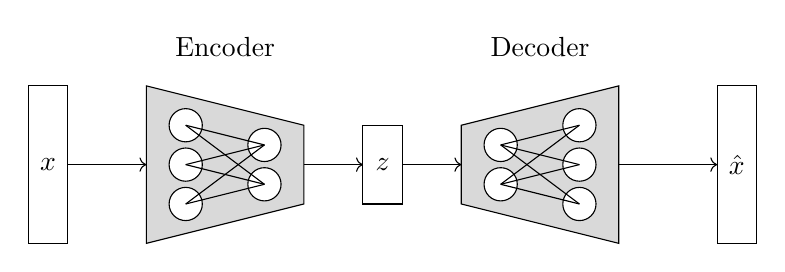
\begin{tikzpicture}
        % Center point of encoder
        \coordinate (E_CENTER) at (1, 1);
        \coordinate (INPUT_TEXT) at (-0.25, 0.5);



        % Draw input vector
        \draw ($(INPUT_TEXT) + (-0.25, -0.5)$) rectangle ($(INPUT_TEXT) + (0.25, 1.5)$) node[pos=.5] {$x$};
        \draw[->] ($(E_CENTER) + (-1, 0)$) -- (E_CENTER);

        








        % Draw the encoder
        \node at ($(E_CENTER) + (1, 1.5)$) {Encoder};
        
        \coordinate (A) at ($(E_CENTER) + (0, -1)$);
        \coordinate (B) at ($(E_CENTER) + (2, -0.5)$);
        \coordinate (C) at ($(E_CENTER) + (2, 0.5)$);
        \coordinate (D) at ($(E_CENTER) + (0, 1)$);
        \draw[fill=gray!30] (A) -- (B) -- (C) -- (D) -- cycle;
        
        % Define the coordinates for the first set of circles (3 neurons)
        \coordinate (n1) at ($(E_CENTER) + (0.5, -0.5)$);
        \coordinate (n2) at ($(E_CENTER) + (0.5, 0)$);
        \coordinate (n3) at ($(E_CENTER) + (0.5, 0.5)$);
        
        % Define the coordinates for the second set of circles (2 neurons)
        \coordinate (m1) at ($(E_CENTER) + (1.5, 0.25)$);
        \coordinate (m2) at ($(E_CENTER) + (1.5, -0.25)$);
        
        % Draw the first set of circles
        \foreach \i in {n1, n2, n3} {
            \filldraw[fill=white] (\i) circle (6pt);
        }
        
        % Draw the second set of circles
        \foreach \i in {m1, m2} {
            \filldraw[fill=white] (\i) circle (6pt);
        }
        
        % Draw arrows from each circle in the first set to each circle in the second set
        \foreach \i in {n1, n2, n3} {
            \foreach \j in {m1, m2} {
                \draw[-] (\i) -- (\j);
            }
        }






        % Draw code vector

        % Arrow in
        \coordinate (Z_TEXT) at ($(E_CENTER) + (3, 0)$);
        \draw[->] ($(E_CENTER) + (2, 0)$) -- ($(Z_TEXT) + (-0.25, 0)$);

        \draw ($(Z_TEXT) + (-0.25, -0.5)$) rectangle ($(Z_TEXT) + (0.25, 0.5)$) node[pos=.5] {$z$};
        
        % Arrow out
        \coordinate (D_CENTER) at ($(E_CENTER) + (4, 0)$);
        \draw[->] ($(Z_TEXT) + (0.25, 0)$) -- (D_CENTER);











        % Draw decoder
        \node at ($(D_CENTER) + (1, 1.5)$) {Decoder};
        
        \coordinate (A2) at ($(D_CENTER) + (0, 0.5)$);
        \coordinate (B2) at ($(D_CENTER) + (2, 1)$);
        \coordinate (C2) at ($(D_CENTER) + (2, -1)$);
        \coordinate (D2) at ($(D_CENTER) + (0, -0.5)$);
        \draw[fill=gray!30] (A2) -- (B2) -- (C2) -- (D2) -- cycle;
        
        % Define the coordinates for the first set of circles (2 neurons)
        \coordinate (n2_1) at ($(D_CENTER) + (0.5, 0.25)$);
        \coordinate (n2_2) at ($(D_CENTER) + (0.5, -0.25)$);
        
        % Define the coordinates for the second set of circles (3 neurons)
        % \coordinate (m2_1) at (1.5, 0.5);
        % \coordinate (m2_2) at (1.5, 1);
        % \coordinate (m2_3) at (1.5, 1.5);
        \coordinate (m2_1) at ($(n2_1) + (1, 0.25)$);
        \coordinate (m2_2) at ($(n2_1) + (1, -0.25)$);
        \coordinate (m2_3) at ($(n2_1) + (1, -0.75)$);
        
        % Draw the first set of circles
        \foreach \i in {n2_1, n2_2} {
            \filldraw[fill=white] (\i) circle (6pt);
        }
        
        % Draw the second set of circles
        \foreach \i in {m2_1, m2_2, m2_3} {
            \filldraw[fill=white] (\i) circle (6pt);
        }
        
        % Draw arrows from each circle in the first set to each circle in the second set
        \foreach \i in {n2_1, n2_2} {
            \foreach \j in {m2_1, m2_2, m2_3} {
                \draw[-] (\i) -- (\j);
            }
        }


        \coordinate (D_END) at ($(D_CENTER) + (2, 0)$);




        % Draw output vector
        \coordinate (X_OUT_TEXT) at ($(m2_2) + (2, 0)$);
        \draw[->] (D_END) -- ($(X_OUT_TEXT) + (-0.25, 0)$);
        
        \draw ($(X_OUT_TEXT) + (-0.25, -1)$) rectangle ($(X_OUT_TEXT) + (0.25, 1)$) node[pos=.5] {$\hat{x}$};
        
        % \node at (X_OUT_TEXT) {$\hat{x}$};
        
    \end{tikzpicture}
    \caption{Autoencoder architecture.}
\end{figure}


More formally, the encoder network takes an input data point $x$ and maps it to a latent space representation $z$, which is compressed representation of $x$. The input is a vector, therefor an image must be flattened from 2D to 1D vector. This flattening will become an issue later in image generation, as this action removes important spatial information and hidden structures in the image. Because of this, modifications were made to the VAE model which allows the capture of spatial information by using a CNN (Convolutional Neural Network) \cite{cnn} layers \cite{vae_cnn_example}, max pooling layers, and more. After compression, the latent vector $z$ is then passed onto the decoder for reconstruction. 

The reconstruction is learned by a reconstruction loss function, usually mean squared error (MSE) loss function:

\begin{equation}
    \text{MSE} = \frac{1}{N} \sum_{i=1}^{N} (y_i - \hat{y}_i)^2
\label{eq:mse}
\end{equation}

The MSE loss is common in image generation models, because this loss is used to ensure that the generated images closely resemble the original input images by comparing the distance between pixels (input image, output image). This objective motivates the model to reconstruct the image from latent vector to resemble the original image. However, this loss is not used alone usually, but in combination with more complex loss functions, as we will see later in VAE.

The code vectors learned by autoencoders, however, are one-to-one map of the input and code vector (deterministic mapping from input to code vectors). The model doesn't capture any semantic relationships between the data (e.g the code vectors of images of cats are scattered throughout the entire latent space, whereas in VAE, they are clustered together). The latent space in autoencoders is irregular and discontinuous, meaning a small change in the latent vector can lead to large unpredictable changes in the output. This makes interpolation in the latent space difficult. Variational autonecoder solve this problem. VAE regularizes the latent space by enforcing a prior distribution. This regularization leads to a smooth and continuous latent space (see figure \ref{fig:ae_vs_vae}), which allows the model to interpolate between the latent space smoothly, thus creating similar new images with different variations. VAEs also provide an explicit model of the data distribution by maximizing a variational lower bound on the likelihood of the data. In other words, VAE is probabilistic model instead of discrete mapper (like the autoencoder model).

\begin{figure}[h]
    \centering
    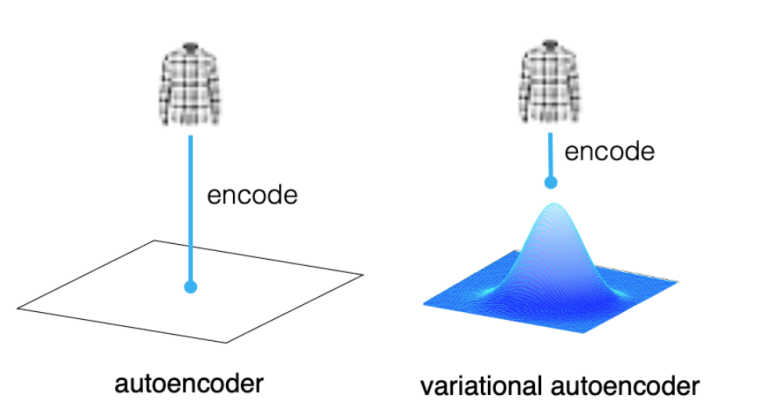
\includegraphics[scale=0.5]{images/autoencoder-vs-variational-autoencoder-point-vs-distribution-768x409.png}
    \caption{Illustration of mapping an input image to code vector (left) and mapping an input image to a distribution (right) \cite{ae_vs_vae}.}
    \label{fig:ae_vs_vae}
\end{figure}

At the heart of VAE lies the concept of latent variables (Appendix \ref{appendix:latent_variables}). Latent variables are hidden, unobserved variables that the model infers from the observed data (dataset). Latent variable models, such as VAE, take indirect approach to describing a probability distribution $p(x)$ over multi-dimensional variable $x$. Instead of directly writing the expression for $p(x)$, they model a joint distribution $p(x|z)$ of the data $x$ and an unobserved hidden latent variable $z$.

The variational aspect of VAE refers to the use of variational inference (VI) (Appendix \ref{appendix:variational_inference}). VI is used to used to approximate complex posterior distributions: 

\begin{equation}
p(z|x) = \frac{p(x|z) \cdot p(z)}{\int p(x|z) \cdot p(z) dz}
\label{eq:posterior}
\end{equation}

by transforming the problem into optimization problem. The denominator in eq. \ref{eq:posterior} is intractable because it involves integrating over all possible values of $z$, and $z$ is often relatively high-dimensional and its infeasible to evaluate exactly. Which is why VI is used, which approximates the true posterior distribution $p(z|x)$ with simpler, tractable distribution $q_\phi (z|x)$, parameterized by $\phi$.

The original VAE model uses fully connected layers at the encoder and decoder networks. However, in the image synthesis field, CNN layers (appendix \ref{appendix:cnn}) are used instead which are computationally less expensive and better capture the spatial information, for instance, its used in VQ-VAE (section \ref{sec:vqvae}) and PixelCNN \cite{pixelcnn}.

To generate an image, we first sample a latent variable $z$ from prior distribution $p(z)$, which is typically standard normal distribution $\mathcal{N}(0, 1)$. Then $z$ is passed to the decoder an an image $x$ is generated from the conditional distribution $p_\theta (x|z)$. 

\subsection{The Reparameterization Trick}
To enable backpropagation through the sampling process, VAEs use the reparameterization trick. This trick involves expressing the sampled latent variables $z$ as a deterministic function of the encoder's output and some random noise. Without this technique, backpropagation would not be possible through the sampling operation. The reason is that sampling is a non-differentiable operation, because sampling from a distribution involves randomness that does not have a gradient, and the gradients cannot be computed with respect to the parameters of the encoder. To make the sampling operation differentiable and thus allow gradients to flow through the network, the reparameterization trick is used. 

Specifically, if $\mu$ and $\sigma$ are the mean and standard deviation vectors outputted by the encoder, we can write:

\begin{equation}
    z = \mu + \sigma \cdot \epsilon
\end{equation}

where $\epsilon \sim \mathcal{N}(0, 1)$ is a standard normal random variable. This $\epsilon$ will not change throughout the training reigime. It is sampled once and fixed in place. This trick allows us instead of having full stochastic node that blocks flow of gradients, to having two parts: one where we can do backpropagation, and another part which is still stochastic but which we don't want to train because its fixed.


\begin{figure}[h]
    \centering
    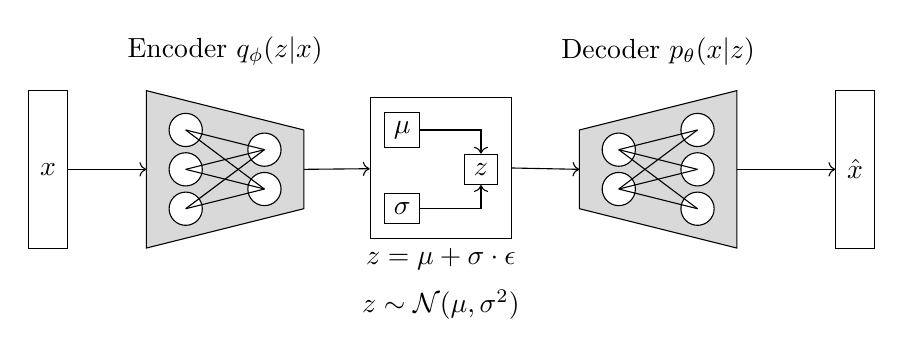
\begin{tikzpicture}
        % Center point of encoder
        \coordinate (E_CENTER) at (1, 1);
        \coordinate (INPUT_TEXT) at (-0.25, 0.5);



        % Draw input vector
        \draw ($(INPUT_TEXT) + (-0.25, -0.5)$) rectangle ($(INPUT_TEXT) + (0.25, 1.5)$) node[pos=.5] {$x$};
        \draw[->] ($(E_CENTER) + (-1, 0)$) -- (E_CENTER);

        








        % Draw the encoder
        \node at ($(E_CENTER) + (1, 1.5)$) {Encoder $q_\phi(z|x)$};
        
        \coordinate (A) at ($(E_CENTER) + (0, -1)$);
        \coordinate (B) at ($(E_CENTER) + (2, -0.5)$);
        \coordinate (C) at ($(E_CENTER) + (2, 0.5)$);
        \coordinate (D) at ($(E_CENTER) + (0, 1)$);
        \draw[fill=gray!30] (A) -- (B) -- (C) -- (D) -- cycle;
        
        % Define the coordinates for the first set of circles (3 neurons)
        \coordinate (n1) at ($(E_CENTER) + (0.5, -0.5)$);
        \coordinate (n2) at ($(E_CENTER) + (0.5, 0)$);
        \coordinate (n3) at ($(E_CENTER) + (0.5, 0.5)$);
        
        % Define the coordinates for the second set of circles (2 neurons)
        \coordinate (m1) at ($(E_CENTER) + (1.5, 0.25)$);
        \coordinate (m2) at ($(E_CENTER) + (1.5, -0.25)$);
        
        % Draw the first set of circles
        \foreach \i in {n1, n2, n3} {
            \filldraw[fill=white] (\i) circle (6pt);
        }
        
        % Draw the second set of circles
        \foreach \i in {m1, m2} {
            \filldraw[fill=white] (\i) circle (6pt);
        }
        
        % Draw arrows from each circle in the first set to each circle in the second set
        \foreach \i in {n1, n2, n3} {
            \foreach \j in {m1, m2} {
                \draw[-] (\i) -- (\j);
            }
        }






        % Draw middle
        \coordinate (Z_TEXT) at ($(E_CENTER) + (3, 0)$);

        \coordinate (MIDDLE_BEGIN) at ($(Z_TEXT) + (-0.5, 0)$);
        \coordinate (MU_BEGIN) at ($(MIDDLE_BEGIN) + (0.25, 0.5)$);
        \coordinate (SIGMA_BEGIN) at ($(MIDDLE_BEGIN) + (0.25, -0.5)$);
        \coordinate (Z_BEGIN) at ($(Z_TEXT) + (0.75, 0)$);

        \coordinate (ARROW_OUT_BEGIN) at ($(Z_TEXT) + (1.75, 0)$);
        \coordinate (ARROW_OUT_END) at ($(ARROW_OUT_BEGIN) + (0.5, 0)$);

        % Middle nodes
        \node[draw,rectangle] (SIGMA) at ($(SIGMA_BEGIN) + (0.5, 0)$) {$\sigma$};
        \node[draw,rectangle] (MU) at ($(MU_BEGIN) + (0.5, 0)$) {$\mu$};
        \node[draw,rectangle] (Z) at ($(Z_BEGIN) + (0.5, 0)$) {$z$};

        % Rectangle around all nodes
        \node[draw, rectangle, inner sep=5pt, fit=(SIGMA) (MU) (Z)] (middle_rect) {};

        % Equations below the rectangle
        \node[below=0cm of middle_rect] (eq1) {$z = \mu + \sigma \cdot \epsilon$};
        \node[below=0cm of eq1] (eq2) {$z \sim \mathcal{N}(\mu, \sigma^2)$};

        % Arrow from trapazoid to rectangle
        \draw[->] ($(E_CENTER) + (2, 0)$) -- (middle_rect);

        % Inner arrows
        \draw[->, to path={-| (\tikztotarget)}] (SIGMA) edge (Z) (MU) edge (Z);











        % Draw decoder
        \coordinate (D_CENTER) at ($(Z_TEXT) + (2.5, 0)$);
        \node at ($(D_CENTER) + (1, 1.5)$) {Decoder $p_\theta(x|z)$};

        % Arrow from the rectangle to the trapezoid
        \draw[->] (middle_rect.east) -- (D_CENTER);

        % Draw trapazoid
        \coordinate (A2) at ($(D_CENTER) + (0, 0.5)$);
        \coordinate (B2) at ($(D_CENTER) + (2, 1)$);
        \coordinate (C2) at ($(D_CENTER) + (2, -1)$);
        \coordinate (D2) at ($(D_CENTER) + (0, -0.5)$);
        \draw[fill=gray!30] (A2) -- (B2) -- (C2) -- (D2) -- cycle;
        
        % Define the coordinates for the first set of circles (2 neurons)
        \coordinate (n2_1) at ($(D_CENTER) + (0.5, 0.25)$);
        \coordinate (n2_2) at ($(D_CENTER) + (0.5, -0.25)$);
        
        % Define the coordinates for the second set of circles (3 neurons)
        \coordinate (m2_1) at ($(n2_1) + (1, 0.25)$);
        \coordinate (m2_2) at ($(n2_1) + (1, -0.25)$);
        \coordinate (m2_3) at ($(n2_1) + (1, -0.75)$);
        
        % Draw the first set of circles
        \foreach \i in {n2_1, n2_2} {
            \filldraw[fill=white] (\i) circle (6pt);
        }
        
        % Draw the second set of circles
        \foreach \i in {m2_1, m2_2, m2_3} {
            \filldraw[fill=white] (\i) circle (6pt);
        }
        
        % Draw arrows from each circle in the first set to each circle in the second set
        \foreach \i in {n2_1, n2_2} {
            \foreach \j in {m2_1, m2_2, m2_3} {
                \draw[-] (\i) -- (\j);
            }
        }


        \coordinate (D_END) at ($(D_CENTER) + (2, 0)$);

        % Draw output vector
        \coordinate (X_OUT_TEXT) at ($(m2_2) + (2, 0)$);
        \draw[->] (D_END) -- ($(X_OUT_TEXT) + (-0.25, 0)$);
        
        \draw ($(X_OUT_TEXT) + (-0.25, -1)$) rectangle ($(X_OUT_TEXT) + (0.25, 1)$) node[pos=.5] {$\hat{x}$};
        
        % \node at (X_OUT_TEXT) {$\hat{x}$};
        
    \end{tikzpicture}
    \caption{Variational Autoencoder architecture.}
    \label{figure:vae}
\end{figure}


The VAE architecture is shown in figure \ref{figure:vae}.

\subsection{Training}

The VAE optimizes the Evidence Lower Bound (ELBO) (see appendix \ref{appendix:elbo}) to ensure that the approximate posterior $q_\phi (z|x)$ is close to the true posterior $p(z|x)$ (we want to maximize it):

\begin{equation}
    \mathcal{L}(\theta, \phi; x, z) = \text{ELBO} = \mathbb{E}_{q_\phi(z|x)} \left[ \log p_\theta(x|z) \right] - D_\text{KL}(q_\phi(z|x) \| p(z))
\end{equation}

where the first term is the reconstruction loss and the second term is the KL divergence (see appendix \ref{appendix:kl_divergence}) (which measure how much the approximate posterior $q_\phi (z|x)$ diverges from the prior $p(z)$). 

% VQ-VAE
\section{VQ-VAE}
\label{sec:vqvae}

Vector Quantized Variational Autoencoder (VQ-VAE) \cite{vqvae} is a generative models based on VAE \ref{sec:vae} model with the addition of vector quantization (VQ) (section \ref{subsec:vqvae_vq}) technique. 

\subsection{Vector Quantization}
\label{subsec:vqvae_vq}

Vector quantization (VQ) is a technique used to discretize continuous data. In the context of VQ-VAE, the continuous latent space $z$ is mapped into discrete codes vectors. In a continuous latent space, the amount of possibilities for a value in the hidden space is infinite, which makes it difficult for the model to learn the hidden space efficiently. With a discrete hidden space, learning becomes more efficient because there is a fixed number of possible values (although in reality it is very large, for example the amount of objects that can be described using language is finite but very large). Furthermore, in reality, images are divided into classes of objects such as cats, people, dogs, etc., and each class has a finite number of possibilities, which is better suited to a discrete latent vectors.

\begin{figure}[h]
    \centering
    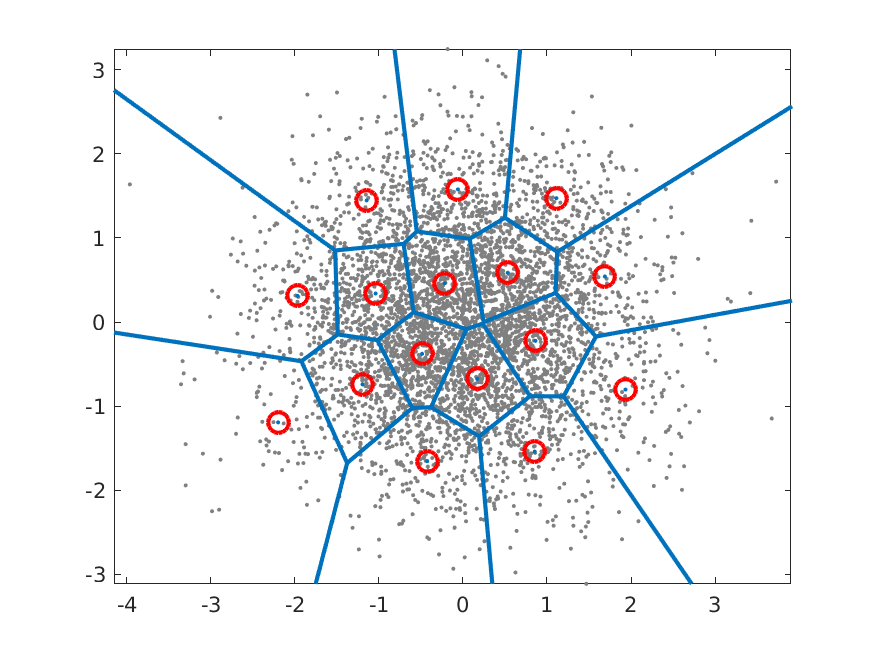
\includegraphics[scale=0.5]{images/vq_visualization.png}
    \caption{Illustration of vector quantization discrete clustering of the 2D latent space \cite{vq_visualization_website}. The grey dots are embeddings of the continous latent space, and the red dots are the code vectors from the codebook. In this case, the codebook size is 16.}
    \label{figure:vq_visualization}
\end{figure}

This technique involves the use of a codebook, which is a discrete collection of vectors of the same size as the hidden dimension. In the VQ-VAE model, after the input passes through the encoder (which results in embeddings - which are the hidden representation of the input), the embeddings are replaced by the closest vector from the codebook (by minimizing distance between vectors). This operation allows the model to learn clusters of similar embeddings, which can be used to generate new samples. The codebook is learned during training, and the embeddings are quantized to the nearest code vector in the codebook. The codebook is learned by minimizing the loss function:

\begin{equation}
    \mathcal{L}_{\text{VQ}} = || \text{sg}[z_e] - z_q ||_2^2 + \beta || \text{sg}[z_q] - z_e ||_2^2
\label{eq:vq_loss}
\end{equation}

where $z_e$ is the encoder output, $z_q$ is the quantized output, $\text{sg}[\cdot]$ is the stop gradient operation (which prevents gradients from flowing through the quantization operation), and $\beta$ is a hyperparameter that controls the weighting of the two terms in the loss function. The first term in the loss function is the quantization loss, which measures the distance between the encoder output and the quantized output. The second term is the commitment loss, which measures the distance between the quantized output and the encoder output. The commitment loss encourages the model to use the codebook, and prevents the model from ignoring the quantization operation.

\subsection*{Architecture}

ABC

\subsection*{Training}

ABC

% GAN
\section{Generative Adversarial Networks (GANs)}
\label{sec:gan}

\begin{figure}
    \centering
    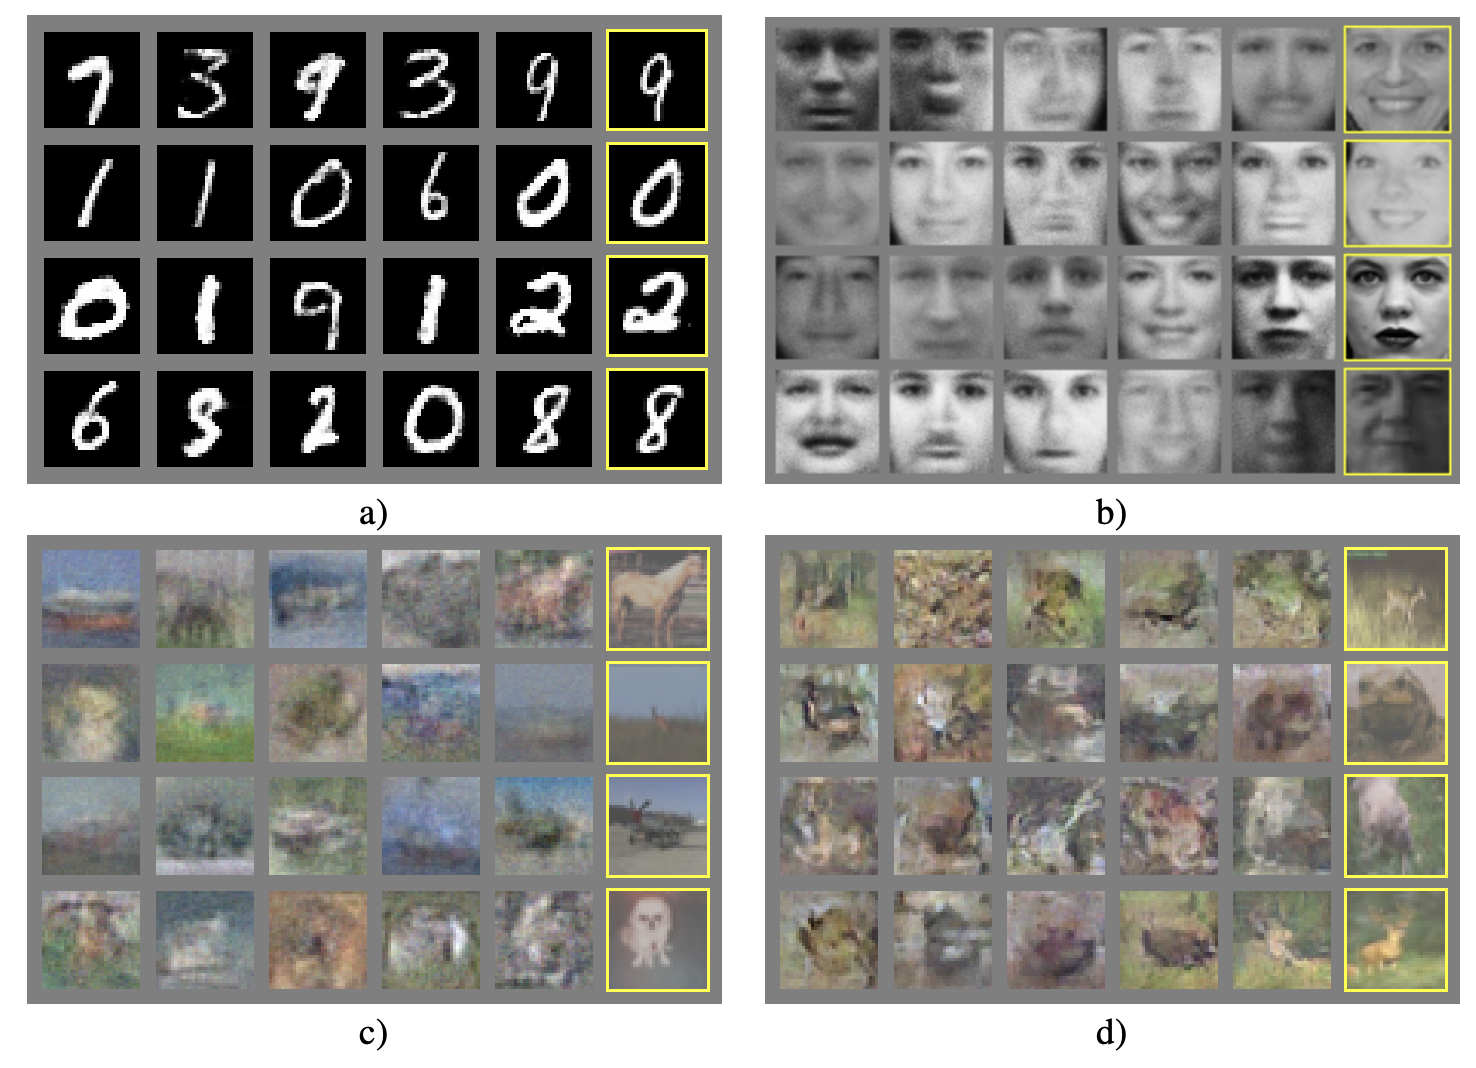
\includegraphics[width=0.75\textwidth]{images/gan_samples.png}
    \caption{Some samples generated by GAN in the paper \cite{gan}. Right: samples from the training data. Left: samples generated by the model. a) is from the MNIST dataset, b) is from the Toronto Face Database (TFD), c) is from the CIFAR-10 dataset with fully-connected layers at the generator and discriminator, and d) is from the CIFAR-10 dataset with convolutional layers at the generator and discriminator.}
\end{figure}

Generative Adversarial Networks (GANs) \cite{gan} are a class of deep learning models that are used to generate new data samples from a given distribution. More specifically, they are very good at synthesizing high-quality images. The model can be used by itself, or as we will see later, it can also be the basis of other image and video generation models, such as VQ-GAN \ref{sec:vqgan}.

\begin{figure}
    \centering
    \resizebox{\textwidth}{!}{
        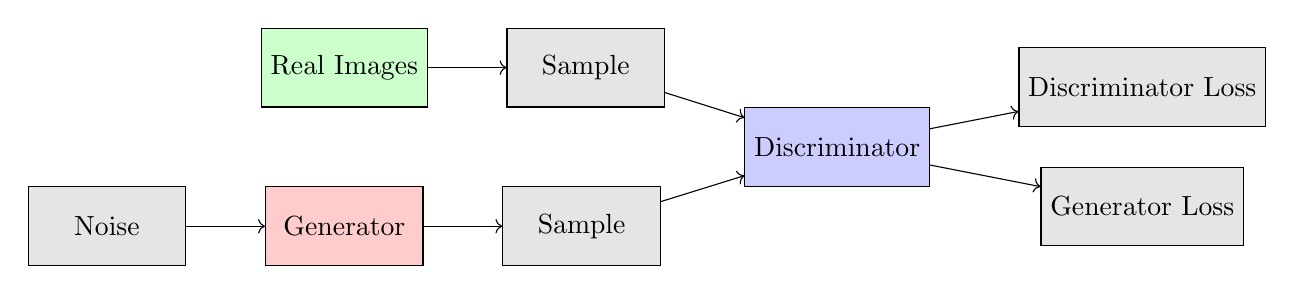
\begin{tikzpicture}
            % Real images, Generator nodes
            \node[rectangle, draw, fill=green!20, minimum width=2cm, minimum height=1cm] (real_images) {Real Images};
            \node[rectangle, draw, fill=red!20, minimum width=2cm, minimum height=1cm, below=of real_images] (generator) {Generator};

            % Noise node
            \node[rectangle, draw, fill=gray!20, minimum width=2cm, minimum height=1cm, left=of generator] (noise) {Noise};

            % Arrow from noise to generator
            \draw[->] (noise) -- (generator);

            % Sample nodes
            \node[rectangle, draw, fill=gray!20, minimum width=2cm, minimum height=1cm, right=of generator] (sample_gen) {Sample};
            \node[rectangle, draw, fill=gray!20, minimum width=2cm, minimum height=1cm, right=of real_images] (sample_real_images) {Sample};

            % Fit sample nodes in a box
            \node[fit=(sample_gen)(sample_real_images), inner sep=0] (sample_fitbox) {};


            % Arrows to sample nodes
            \draw[->] (real_images) -- (sample_real_images);
            \draw[->] (generator) -- (sample_gen);

            % Discriminator node
            \node[rectangle, draw, fill=blue!20, minimum width=2cm, minimum height=1cm, right=of sample_fitbox] (discriminator) {Discriminator};

            % Arrows to discriminator
            \draw[->] (sample_real_images) -- (discriminator);
            \draw[->] (sample_gen) -- (discriminator);

            % Discriminator loss, Generator loss
            % Matrix for the nodes to the right
            \matrix[
                right=of discriminator, 
                column sep=0.5cm, 
                row sep=0.5cm, 
                nodes={rectangle, draw, minimum width=4cm, minimum height=2cm, anchor=center}
            ] (matrix) {
                \node[rectangle, draw, fill=gray!20, minimum width=2cm, minimum height=1cm] (discriminator_loss) {Discriminator Loss}; \\
                \node[rectangle, draw, fill=gray!20, minimum width=2cm, minimum height=1cm] (generator_loss) {Generator Loss}; \\
            };

            % Add arrows
            \draw[->] (discriminator) -- (discriminator_loss);
            \draw[->] (discriminator) -- (generator_loss);
        \end{tikzpicture}
    }
    \caption{GAN architecutre \cite{gan}. Noise is sampled from a noise distribution and fed to the generator. The generator outputs an image, and the discriminator needs to decide if the image was generated by the generator or if its an image from the dataset. This decision then affects the value of the loss function, and the weights are updated accordingly by backpropogation.}
    \label{fig:gan_architecture}
\end{figure}

% TODO: \ref{fig:gan_architecture} is referencing to the GAN section, and not the figure! WTF
The model consists of two neural networks: a generator $G$ and a discriminator $D$ (as shown in figure \ref{fig:gan_architecture}). The generator is responsible for generating new samples $x$ (images), while the discriminator is responsible for distinguishing between real samples (from the dataset, $D(x) = 1$) and generated samples (fake, from the generator, $D(x) = 0$). The two networks are trained simultaneously in a minimax game (see training section \ref{subsec:gan_training}), where the generator tries to generate samples that are indistinguishable from real samples, and the discriminator tries to distinguish between real and generated samples. The training process continues until the generator is able to generate realistic and high-quality images. 

The noise vector is sampled from a simple distribution like Gaussian. The basic idea of using noise as input is that the model learns to establish relationships between each dimension in the vector and the output image, similar to latent vectors or code vectors. For instance, the model might learn that the first dimension of the noise vector corresponds to the shape of the middle of the image (like the shape of the head of a person), while the second dimension might corresponds to the color of the shape, and so on.




\subsection{Training}
\label{subsec:gan_training}

The loss function of the GAN model is defined as the following min-max game:

\begin{equation}
    \label{eq:gan_loss}
    \min_G \max_D V(D,G) = \mathbb{E}_{x \sim p_{\text{data}}(x)}[\log D(x)] + \mathbb{E}_{z \sim p_z(z)}[\log(1 - D(G(z)))]
\end{equation}

We have two prior distributions: $x \sim p_{\text{data}}$ and $z \sim p_z(z)$, where the noise vector $z$ is sampled from a noise distribution, and $p_{\text{data}}$ represents the true underlying distribution of the dataset, and $x$ is sampled from this distribution.

With respect to the discriminator gradients, the loss function tries to maximize the probability that:

\begin{enumerate}
    \item the discriminator correctly classifies real samples as real (the first term)
    \item the discriminator correctly classifies generated samples as fake (the second term)
\end{enumerate}


With respect to the generator gradients \footnote{When we do backpropogation with respect to the generatoe gradients, the first term is constant.}, the loss function tries to minimize the probability that:

\begin{enumerate}
    \item the generator tries to fool the discriminator in thinking that the generated samples are real (the second term)
\end{enumerate}


The researchers mentioned that at the beginning of the training, the discriminator rejects samples with high confidense. To address this, they suggested instead of \textbf{minimizing} the second term, to \textbf{maximize} a new second term in the loss function: $\log D(G(z))$.


\begin{figure}
    \centering
    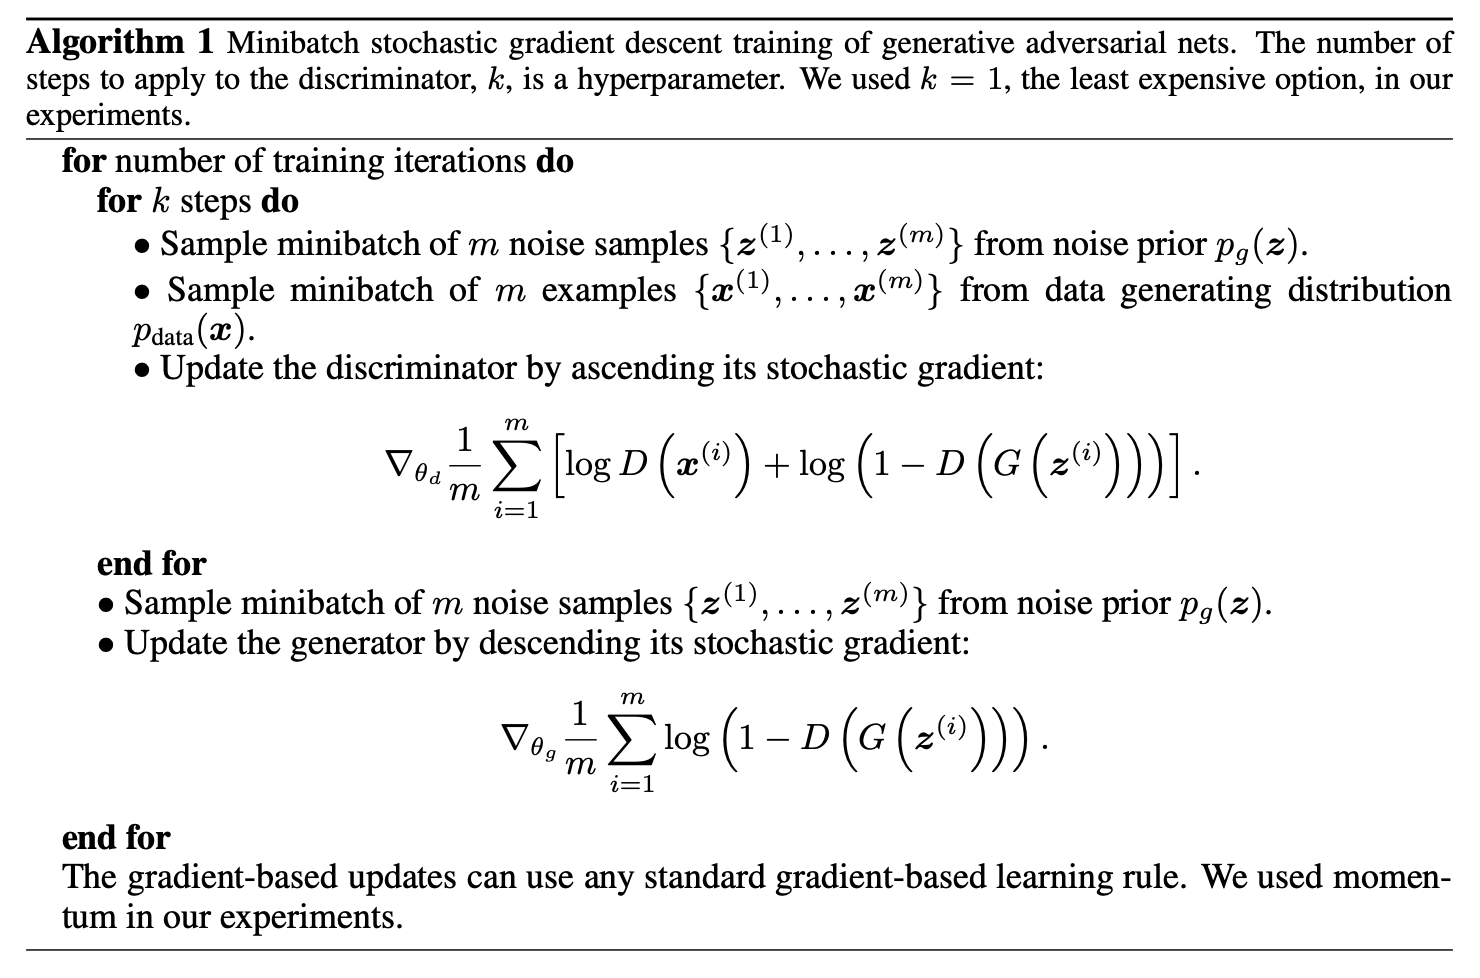
\includegraphics[width=0.75\textwidth]{images/gan_training.png}
    \caption{The training algorithm for GAN using minibatch stochastic gradient decent \cite{gan}.}
    \label{fig:gan_training}
\end{figure}

In order to balance of the training for both $G$ and $D$ the authors suggested using iterative approach using minibatch stochastic gradient decent (see figure \ref{fig:gan_training}). Instead of fully optimizing $D$ in each iteration, the algorithm alternates between a few steps ($k$ steps) of optimizing the discriminator and one step of optimizing the generator. By updating $D$ more often the researchers hope to update the generator more slowly and stabilize the training process.



\subsection{Mode Collapse}

One of the main challenges of training GANs is mode collapse. Mode collapse occurs when the generator learns to generate only a few samples, instead of learning to generate a diverse set of samples. This can happen when the generator learns to generate samples that fool the discriminator, but failed to capture the full diversity of the training data distribution (see figure \ref{fig:gan_mode_collapse}). This can happen when the discriminator is too strong, and the generator is not able to generate diverse samples. In other words, the generator tries to fool the discriminator so much that it only focuses on this goal, while ignoring to diversify the samples.

\begin{figure}
    \centering
    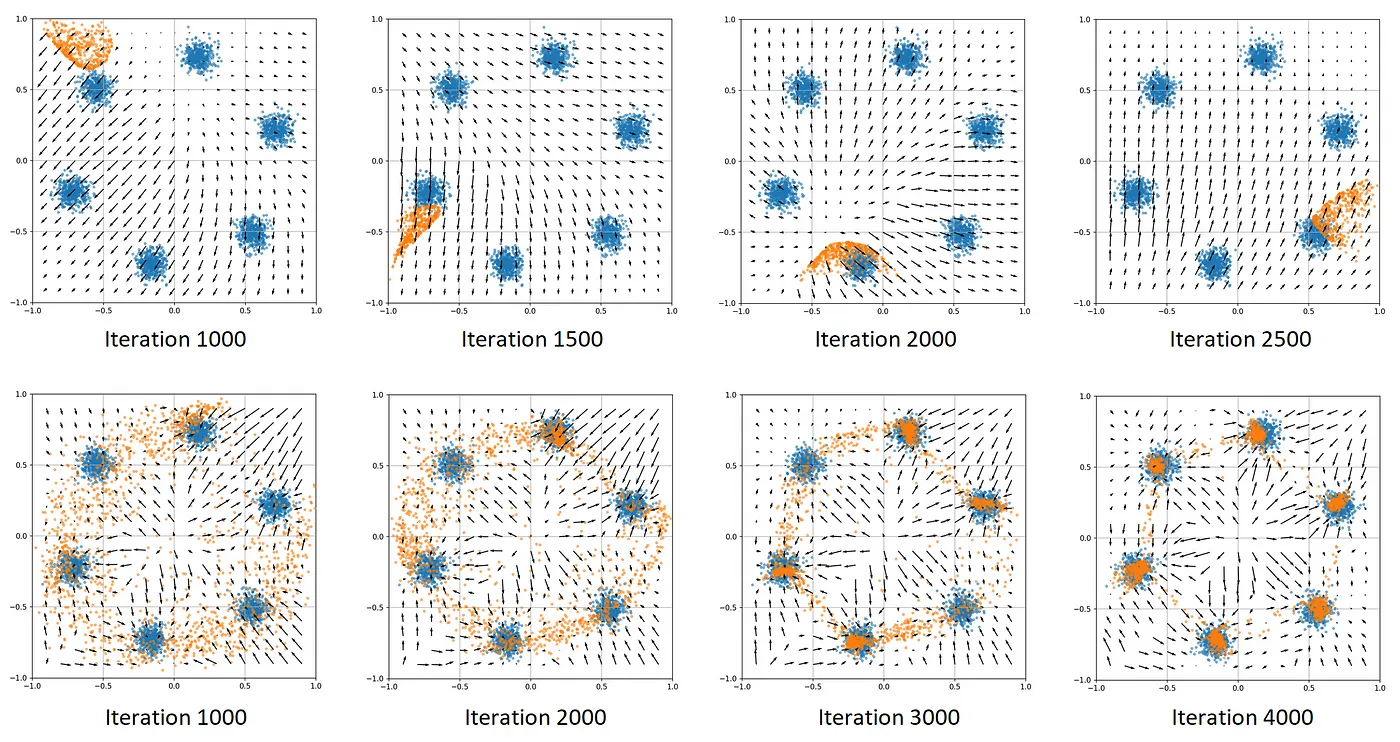
\includegraphics[width=\textwidth]{images/gan_mode_collapse.png}
    \caption{Mode collapse in GANs (top row) \cite{gan_mode_collapse_image_source}. Bottom row shows GAN samples without mode-collapse. Blue dots are the prior $x \sim p_{\text{data}}(x)$ and the orange dots are the generated samples $p_g$.}
    \label{fig:gan_mode_collapse}
\end{figure}


% VQ-GAN
\section{VQ-GAN}
\label{sec:vqgan}

\begin{figure}
    \centering
    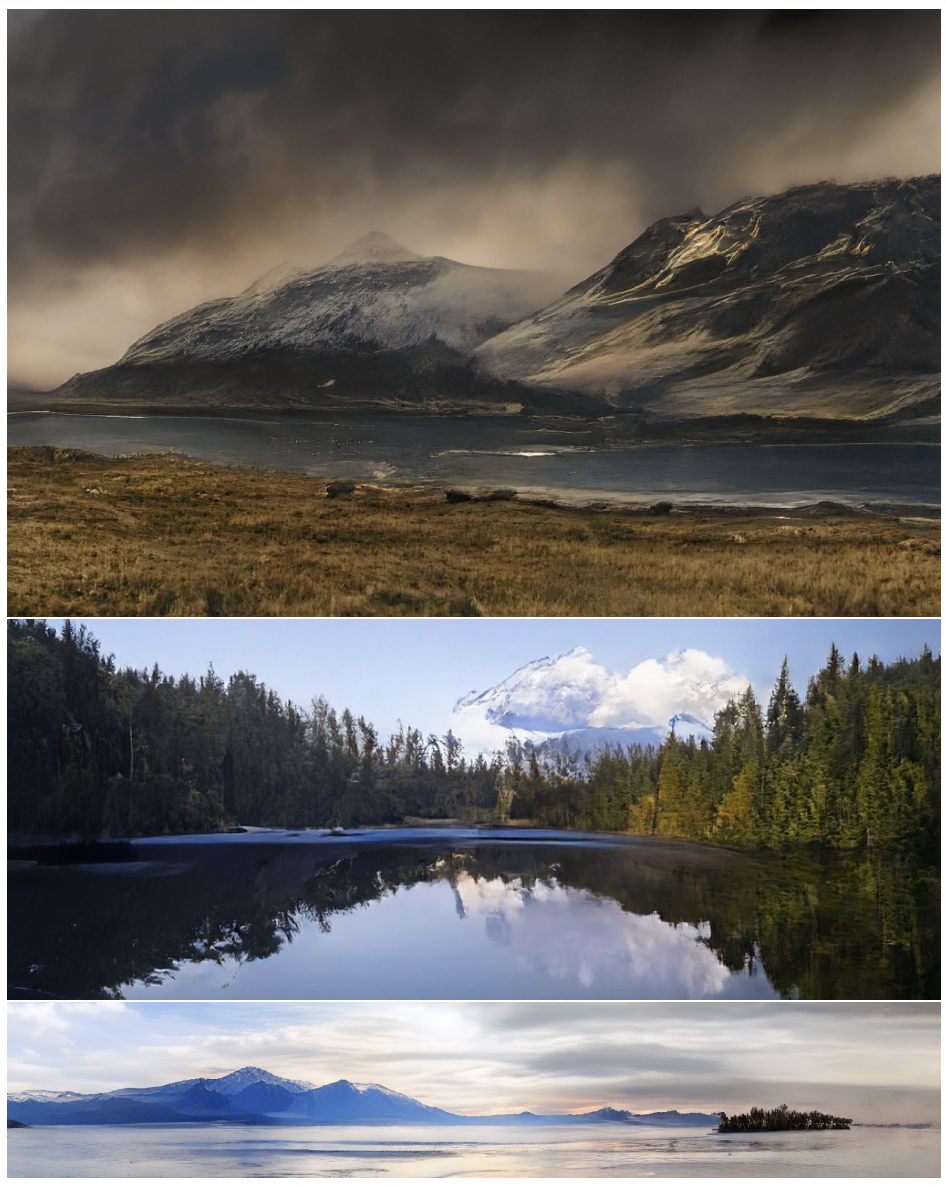
\includegraphics[width=0.5\textwidth]{images/vqgan_samples.png}
    \caption{Samples generated by VQ-GAN with different resolutions (top to bottom: 1280x832, 1024x416, 1280x240), conditioned on semantic layouts from S-FLCKR dataset.}
\end{figure}

Vector Quantized Generative Adversarial Network (VQ-GAN) \cite{vqgan} is a deep learning model capable of generating high-quality images, with the ability of conditioning (text, images, semantic masks and human pose). The architecutre of VQ-GAN is based on previous works: Vector Quantized Variational Autoencoder (VQ-VAE) \cite{vqvae} (section \ref{sec:vqvae}), transformers \cite{transformer} (appendix \ref{appendix:transformers}), and Generative Adversarial Network (GAN) \cite{gan} (section \ref{sec:gan}). The main premises of VQ-GAN is instead of representing an image with pixels, they represent it as a composition of perceptually rich image constituents from a codebook.

VQ-GAN takes the best of both worlds: the ability to generate high-quality images from GANs and the ability to condition the generation process from VQ-VAE using transformers. The combination of the expressivness of transformers and the inductive bias \footnote[1]{Inductive bias is the ability to capture local information in the image, which is why CNN is chosen,  because of the pooling layers.} of CNNs \cite{cnn} in this work showed significant improvements in image generation tasks compared to previous models. Transformers can learn long-range dependencies, whereas CNNs are better fit at learning local features and structures of images. Additional benefit in using a transformer is that is allows the model to output images of various resolutions, which is not possible with previous works.

\begin{figure}
    \centering
    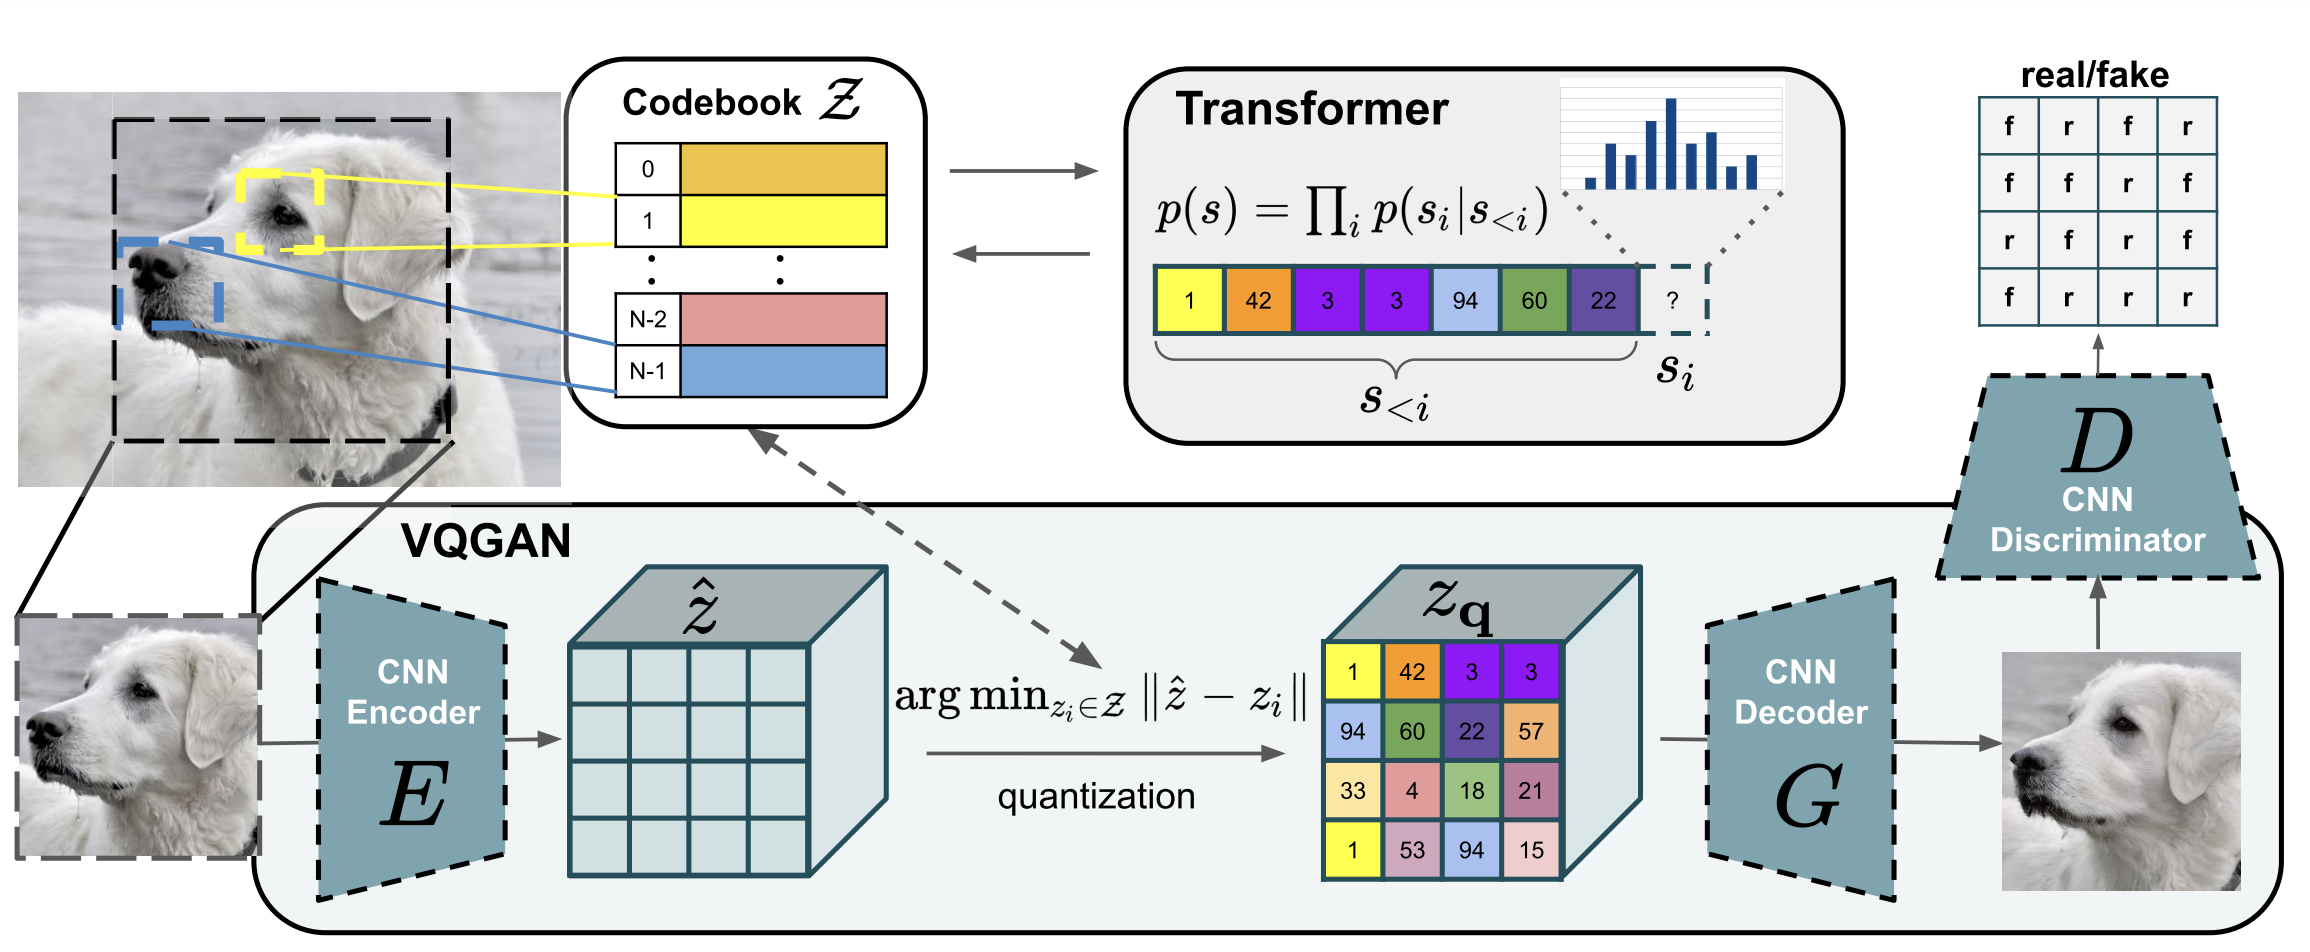
\includegraphics[width=\textwidth]{images/vqgan_architecture.png}
    \caption{VQ-GAN architecture \cite{vqgan}. The bottom rectangular part is the VQ-VAE module with the addition of a descriminator $D$ (right), and the top part is the autoregressive transformer network that predicts the next code vector $s_i$ based on previous outputs $s_{<i}$.}
    \label{fig:vqgan_architecture}
\end{figure}

In the source code of VQ-GAN the researchers used the VGG16 \cite{vgg16} architecture as the backbone of the encoder and decoder networks, but they mentioned that other architectures can be used as well, depending on the generative task. In addition, the authors used the minGPT \cite{mingpt} architecture as the transformer module (more commonly known as GPT-2, which is based on the OpenAI's model GPT-1).

The non-differential operation of quantization is a problem we saw previously in VQ-VAE (subsection \ref{subsec:vqvae_vq}), and to solve this problem the authors said that they used the straight-through estimator \cite{ste} to backpropagate the gradients through the quantization process, similarly to VQ-VAE.






\subsection{Architecture}

THe architecture of VQ-GAN is shown in figure \ref{fig:vqgan_architecture}. The training involves feeding images $x \in X$ of size $x \in \mathbb{R}^{H \times W \times 3}$ \footnote[2]{The training dataset was of size $256 \times 256 \times 3$.} to the encoder $E$ to get the latent representation $\hat{z}$ of size $\hat{z} \in \mathbb{R}^{h \times w \times n_z}$, where $n_z$ is the dimension of each codebook vector. These representation are then quantisized by the VQ module to get the discrete latent representation $z_q \in \mathbb{R}^{h \times w \times n_z}$. This operation converts latent vectors to indencies of code vectors by nearest neighbor code vector (index in the codebook points to a code vector). Using $z_q$ vectors, the CNN decoder $G$ then reconstructs the image $\hat{x}$. A discriminator $D$ is used to distinguish between real and fake (generated) pixel patches of size 16x16. This module encourages the model to generate finer details and local patterns in the image, leading to better overall quality.

The autoregressive transformer is used to predict the embeddings $z_q$ and provide the decoder $G$ the nessessary information to generate a new image, compared to PixelCNN model \cite{pixelcnn} which uses transformer for pixel-by-pixel prediction.




\subsection{Training}

The model is trained in two stages: in the first phase, the VQ module is trained to learn a discrete latent representation of the input data (learn the codebook), and the second phase trains the transformer module to predict the code vectors sequence that will be used to generate the output image.

The loss function of training the model to learn the codebook is given by: (similar to the VQ-VAE loss function in equation \ref{eq:vqvae_loss}):

\begin{equation}
    \mathcal{L}_{\text{VQ}} (E, G, \mathcal{Z}) = \Vert x - \hat{x} \Vert ^2 + \Vert \text{sg}[E(x)] - z_q \Vert ^2_2 +  \beta \Vert \text{sg}[z_q] - E(x) \Vert ^2_2
\end{equation}

where the first term is the MSE reconstruction loss (similar to equation \ref{eq:mse}), the second term is the quantization error, and the third term is the commitment loss. The reconstruction loss is intended to train the decoder $G$ to output (reconstruct latents $z_q$ to an image) images of similar distribution to the dataset. The quantization loss encourages the model to move the codebook vectors torwards the encoder outputs, so to match the encoder's output distribution (gradients are calculated for $z_q$ and not $\text{sg}[E(x)]$ because of the stop gradient operation). The commitment loss encourages the encoder to "commit" to outputting embeddings that are close to the codebook vectors.

However, instead of the MSE loss, the authors used a perceptual loss \footnote[4]{Perceptual loss measures the difference between the high-level features of two images (a generated image and an image from the dataset). Typically the high-level features are extracted by pretrained CNNs.} and \textbf{introduced an adversarial training procedure with a patch-based discriminator $D$} that tries to distinguish between real and fake pixel patches of size 16x16 of an image. The loss function of the discriminator is given by:

\begin{equation}
    \mathcal{L}_{\text{GAN}}(\{E,G,Z\}, D) = [\log D(x) + \log (1-D(\hat{x}))]
\end{equation}

If $D$ outputs 1, then the image is from the dataset (real), and if it outputs 0, then the image is fake (generated by the decoder $G$). Just like in GAN, the discreiminator objective is to maximize the probability of assigning the correct label to the input image and in the loss function the first term encourages the discriminator to output 1 because $\log D(x)$ approaches 0 when $D(x)$ approaches 1, and the second term encourages the discriminator to output 0 for fake images because $\log (1-D(\hat{x}))$ approaches 0 when $D(\hat{x})$ approaches 0.

Combining both the VQ loss and the adversarial loss, the total loss function is given by:

\begin{equation}
    \mathcal{Q^*} = \arg \min_{E, G, Z} \max_D \mathbb{E}_{x \sim p(x)} [\mathcal{L}_{\text{VQ}} + \lambda \mathcal{L}_{\text{GAN}}]
\end{equation}

The $\lambda$ hyperparameter is used to balance the contribution of adversarial loss relative to the VQ loss.

\begin{figure}
    \centering
    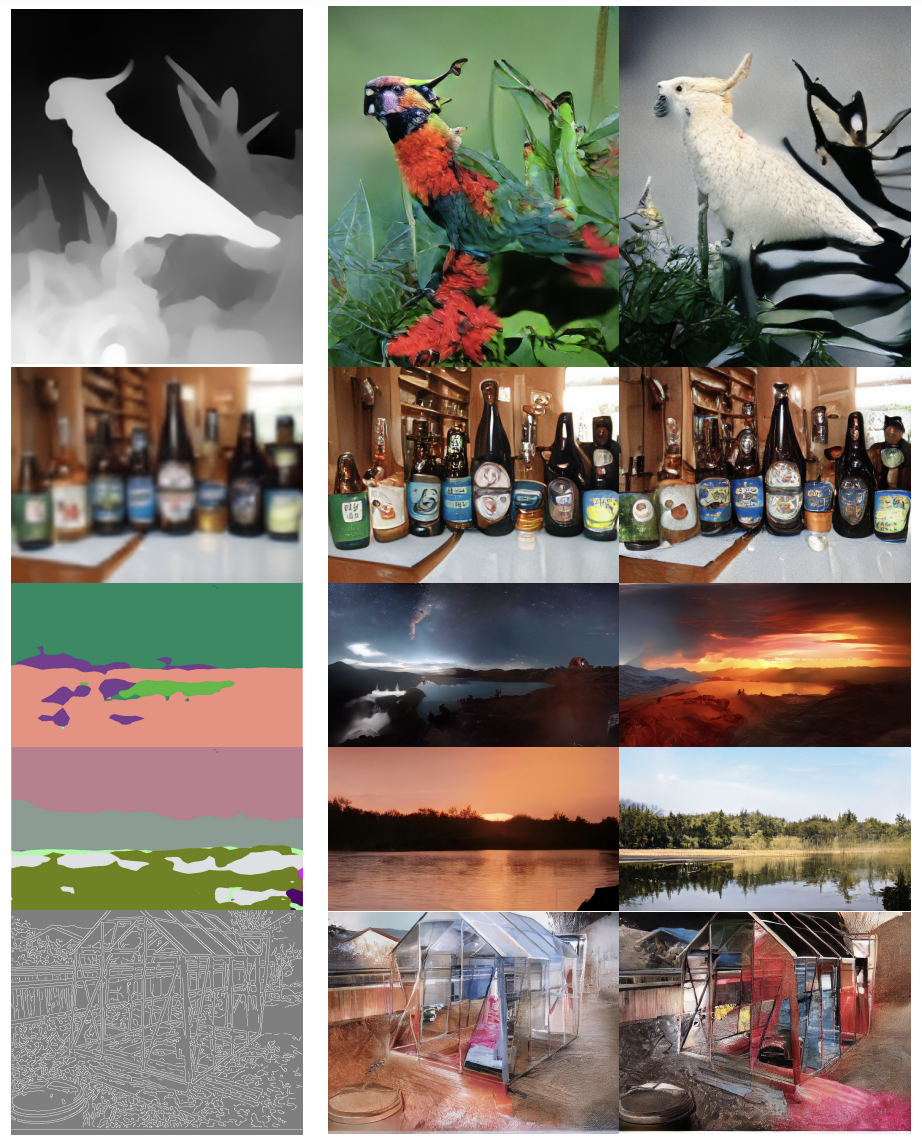
\includegraphics[width=0.5\textwidth]{images/vqgan_samples2.png}
    \caption[Caption for LOF]{Samples generated by VQ-GAN by different tasks and different resolutions. From top to bottom: depth-to-image on RIN dataset, stochastic super resolution\footnotemark on RIN dataset, 3rd and 4th row are semantic synthesis (semantic masks) on S-FLCKR dataset, and bottom row are edge synthesis on IN dataset.}
\end{figure}


\footnotetext{Super resolution is a task that generates high-resolution image from a single low-resolution image while maintaining the spatial information of the image.}

The second phase of the training involves maximizing the transformer objective. The transformer learns to predict the distribution of possible next indices, which allows us to directly maximize the log-likelihood (appendix \ref{appendix:likelihood_function}) of the data representation:

\begin{equation}
    \mathcal{L}_{\text{transformer}} = \mathbb{E}_{x \sim p(x)} [- \log p(x)]
\end{equation}

To summorize, the VQ-GAN model has 3 loss functions: the VQ loss (which trains the model to learn the codebook vectors), the adversarial loss (which trains the model to generate realistic images), and the transformer loss (which trains the model to predict the next code vector autoregressivly).







\subsection{Conditional generation}

% TODO: Finish
After the two-phase training is finished, the transformer is used to predict a sequence $s$ which is sequence of indencies to code vectors. Each token $s_i$ coresponds to an index in the codebook. So a code vector is autoregressivly predicted based on the previous tokens $s_{<i}$, which provides the nessessary embeddings $z_q$ for image synthesis ($p(s) = \prod_{i} p(s_i | s_{<i})$). If the image generation process involves a condition basis $c$, such as text, images, depth map, semantic layout or pose, then another VQ-GAN model is trained on these kind of tasks, which obtain a new codebook $Z_c$ which are the representation $r$ of $c$. Then, this representation is prepended to $s$ which restricts the computation of the negative log-likelihood to entries $p(s_i | s_{<i}, r)$. This new sequence is then given to the transformer in the first model to generate the image based on the condition $c$ (figure \ref{fig:vqgan_conditional_generation}).

\begin{figure}
    \centering
    \label{fig:vqgan_conditional_generation}
    \caption{The conditioned input sequence given to the transformer, based on the spatial condition information $c$. The middle rectangle represents a 'begin sequence' token.}
    
\begin{tikzpicture}
        \def \rectheight{0.5}

        % Draw the first rectangle
        \draw (0,0) rectangle (3,\rectheight);
        \node at (1.5,\rectheight / 2) {r};
        
        % Draw the middle rectangle
        \draw (3,0) rectangle (4,\rectheight);
        
        % Draw the third rectangle
        \draw (4,0) rectangle (7,\rectheight);
        \node at (5.5,\rectheight / 2) {s};
    \end{tikzpicture}
\end{figure}






\subsection{Sliding window technique for generating high-resolution images}

\begin{figure}[h]
    \centering
    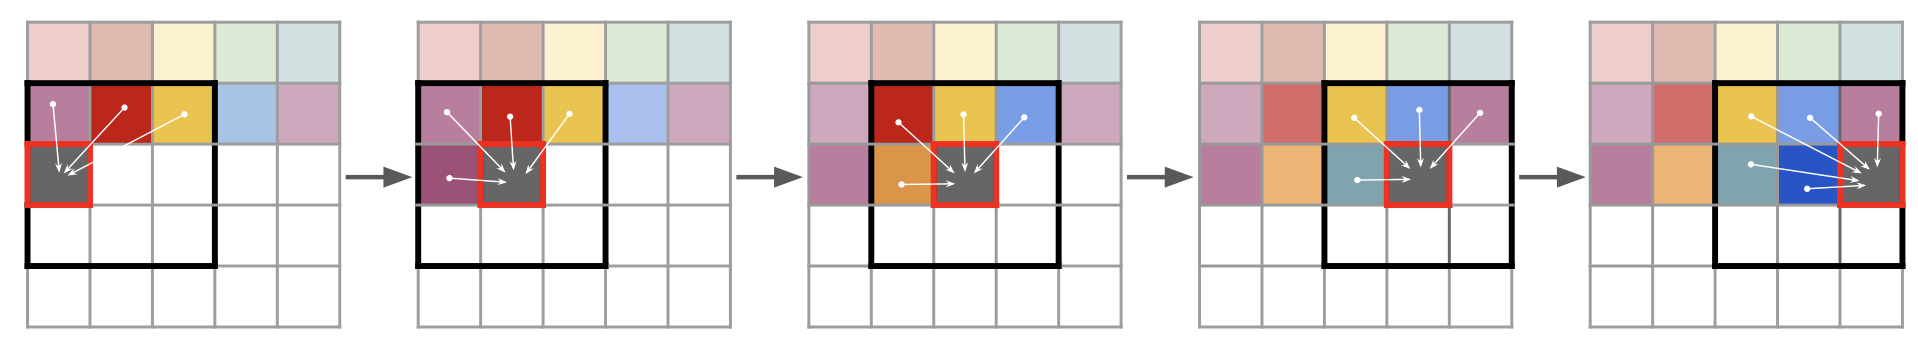
\includegraphics[width=0.75\textwidth]{images/vqgan_sliding_attention.png}
    \caption{Sliding window attention technique for generating high-resolution images. The output image is divided into patches of size 16x16=256 and by using attention mechanism, the transformer module is able to autoregressivly generate the next code vector $s_i$ based on the previous outputs $s_{<i}$ (the context).}
    \label{fig:vqgan_sliding_window}
\end{figure}

Due to the attention mechanism in transformers (quadratic computation for number of tokens, because each token requires attention to all other tokens), the model is limited in the size of the transformer sequence (in the paper they used 256 tokens). Although the encoder can reduce the dimentionality of images, the researchers noticed significant degration in generation quality. To solve this problem, they work patch-wise and crop input images to match the maximum token count in the transformer module.

To sample images, they also work patch-wise and the transformer autoregressivly predicts the next token based on the window context (figure \ref{fig:vqgan_sliding_window}).



% Diffusion models
\section{Denoise Diffusion Probabilistic Models (DDPMs)}


\subsection{Diffusion Models (DMs)}
\label{subsec:diffusion_models}

We previously talked about GANs, VAEs, and their variants (VQ-VAE, VQ-GAN). Diffusion models are also probabilistic models that define a non-linear mapping from latent variables to the observed data. Like variational autoencoders, they approximate the data likelihood using a lower bound. Diffusion models are easy to train and can produce very high-quality images compared to GANs.

A diffusion model consists of two main components: an encoder which takes a data sample $x$ and maps it through a series of intermediate latent variables $z_1, ..., z_T$, and a decoder which reverses this process, until it creates a sample image. The mappings are stochastic rather than discrete (the transformation between the latent variables involve some randomness).

In the next section, we will take a closer look at DDPMs, which is subclass of DMs. Another class of DMs is called Latent Diffusion Models (LDMs) \cite{stable_diffusion} which are based on autoencoders compressing the image space to latent space for more efficient computation.


\subsection{DDPMs}

Denoise Diffusion Probabilistic Models (DDPMs) \cite{ddpm} are a class of diffusion models that are trained to denoise images. In training phase, a dataset of images is fed to the model and DDPMs add noise to input image (it can be thought of as adding random pixel values to the input) in multiple steps (the intermediate latent variables $z_i$), unti the final result is pure noise (which will converge to the noise distribution). Then the model is trained to remove the noise and reconstruct the original image. The denoising process is called 'reverse diffusion' or reverse step and the noising process is called 'forward diffusion' or forward step. The forward diffusion step is denoted as $q(x_t | x_{t-1})$ and the reverse diffusion step is denoted as $p_\theta (x_{t-1} | x_t)$ (figure \ref{fig:ddpm_process}).

Because the addition of noise is a known stochastic process, all the learned parameters are in the decoder (the generator).

Given samples from a data distribution $q(x_0)$ we are interested in learning a model distribution $p_\theta (x_0)$ that approximates $q(x_0)$ and is easy to sample from.

DDPMs are latent variable models in the form of 

\begin{equation}
    p_\theta (x_0) = \int p_\theta(x_{0:T}) dx_{1:T} \text{,\ \ where \ \ \ } p_\theta (x_{0:T}) := p_\theta (x_T) \prod_{t=1}^{T} p_\theta (x_{t-1} | x_t)
\end{equation}

where $x_1, ..., x_T$ are latent variables. Because the integral is intractable, we use ELBO (appendix \ref{appendix:elbo}). The parameters of the model $\theta$ are learned to fit the data distribution $q(x_0)$ by maximizing a variational lower bound:

\begin{equation}
    \max_{\theta} \mathbb{E}_{q(x_0)} [\log p_\theta (x_0)] \leq \max_\theta \mathbb{E}_{q(x_0, x_1, ..., x_T)} [\log p_\theta (x_{0:T}) - \log q(x_{1:T} | x_0)]
\end{equation}

where $q(x_{1:T} | x_0)$ is some inference distribution over the latent variables. Unlike typical latent variable models (such as VAE \ref{sec:vae}), DDPMs are learned with a fixed (rather than trainable) inference procedure $q(x_{1:T} | x_0)$, and latent variables are relatively high dimensional.


\begin{figure}
    \centering
    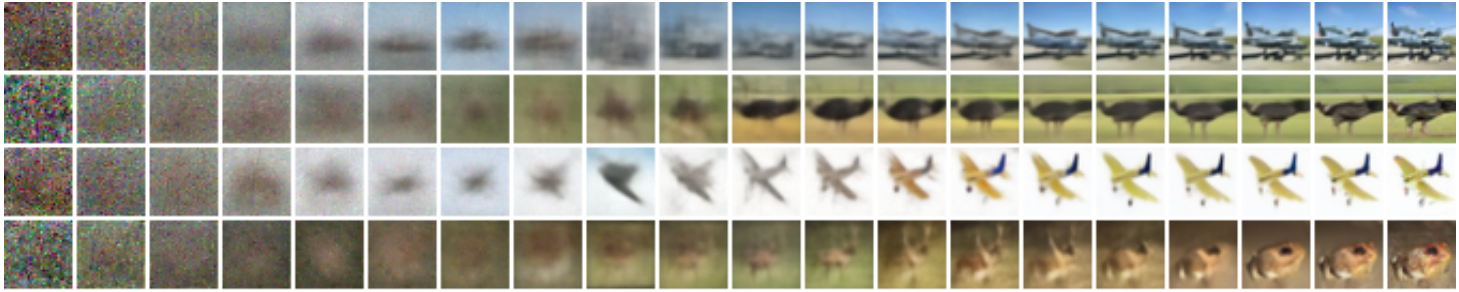
\includegraphics[width=1\textwidth]{images/diffusion_models/ddpm_denoise.png}
    \caption{Progressive generation (left to right) of unconditional CIFAR10 dataset in DDPM \cite{ddpm}.}
\end{figure}


\begin{figure}
    \centering
    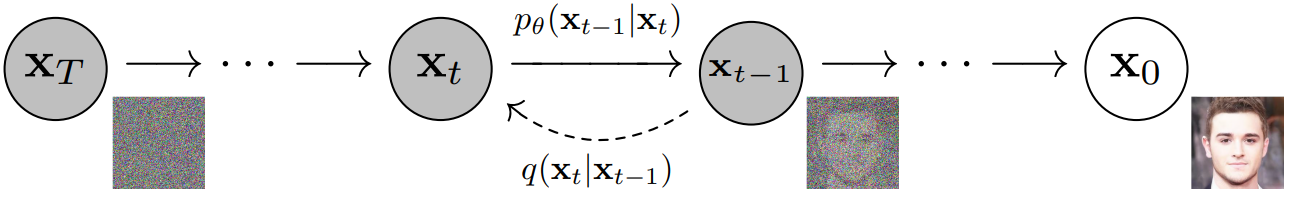
\includegraphics[width=1\textwidth]{images/diffusion_models/ddpm_process.png}
    \caption{A graph representing the forward ($q(x_t | x_{t-1})$) and reverse ($p_\theta(x_{t-1} | x_t)$) diffusion process in DDPMs \cite{ddpm}. The next step (either in forward or reverse diffusion) depends conditionally on the previous steps ($p_\theta (x_{t-1} | x_t)$ is the reverse step, and forward step is $q(x_t | x_{t-1})$).}
    \label{fig:ddpm_process}
\end{figure}






\begin{figure}[h]
    \centering
    \begin{minipage}{0.10\textwidth}  % Divide the width by 7 for 7 images
        \centering
        
\includegraphics[width=\textwidth]{images/diffusion_models/noise_to_image_gif/0.png}
    \end{minipage}
    \begin{minipage}{0.10\textwidth}
        \centering
        
\includegraphics[width=\textwidth]{images/diffusion_models/noise_to_image_gif/1.png}
    \end{minipage}
    \begin{minipage}{0.10\textwidth}
        \centering
        
\includegraphics[width=\textwidth]{images/diffusion_models/noise_to_image_gif/2.png}
    \end{minipage}
    \begin{minipage}{0.10\textwidth}
        \centering
        
\includegraphics[width=\textwidth]{images/diffusion_models/noise_to_image_gif/3.png}
    \end{minipage}
    \begin{minipage}{0.10\textwidth}
        \centering
        
\includegraphics[width=\textwidth]{images/diffusion_models/noise_to_image_gif/4.png}
    \end{minipage}
    \begin{minipage}{0.10\textwidth}
        \centering
        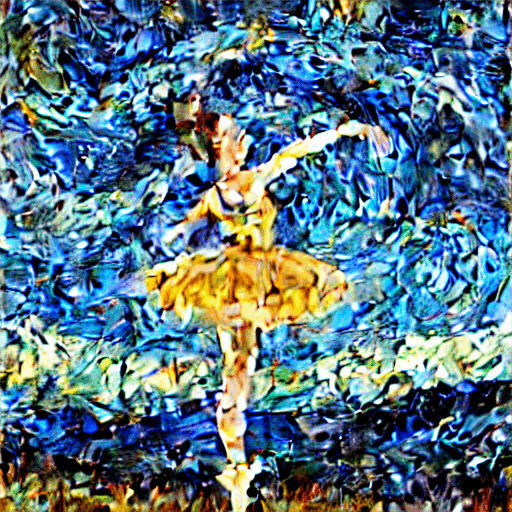
\includegraphics[width=\textwidth]{images/diffusion_models/noise_to_image_gif/5.png}
    \end{minipage}
    \begin{minipage}{0.10\textwidth}
        \centering
        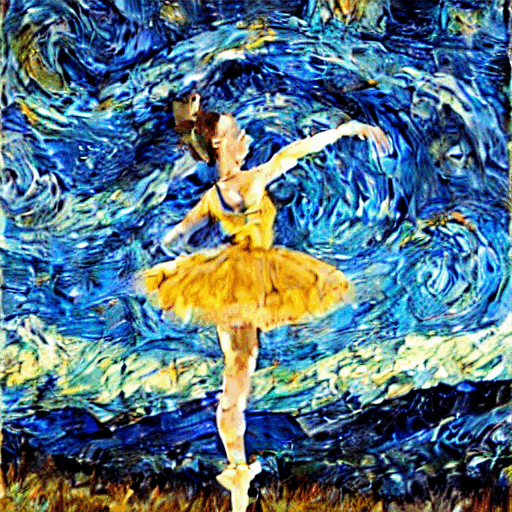
\includegraphics[width=\textwidth]{images/diffusion_models/noise_to_image_gif/6.png}
    \end{minipage}
    \begin{minipage}{0.10\textwidth}
        \centering
        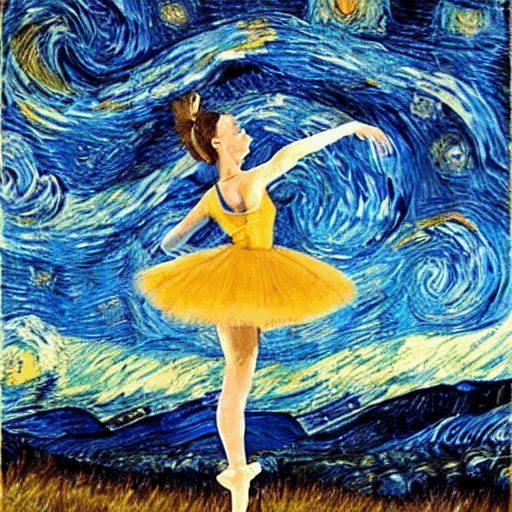
\includegraphics[width=\textwidth]{images/diffusion_models/noise_to_image_gif/7.png}
    \end{minipage}
    \caption{Progressive decoding of noise latents to an image in DDPMs \cite{ddpm}. Images taken from \href{https://scholar.harvard.edu/binxuw/classes/machine-learning-scratch/materials/stable-diffusion-scratch}{harvard university}.}
\end{figure}




\subsection{Noise Schedulers}

In the paper \cite{ddpm} the authors used linear scheduler, however OpenAI released a paper \cite{openai_improved_ddpm} that uses cosine scheduler. They have shown that a cosine scheduler performs better than a linear scheduler in terms of image generation quality (see figure \ref{fig:linear_cosine_scheduler}).

\begin{figure}
    \centering
    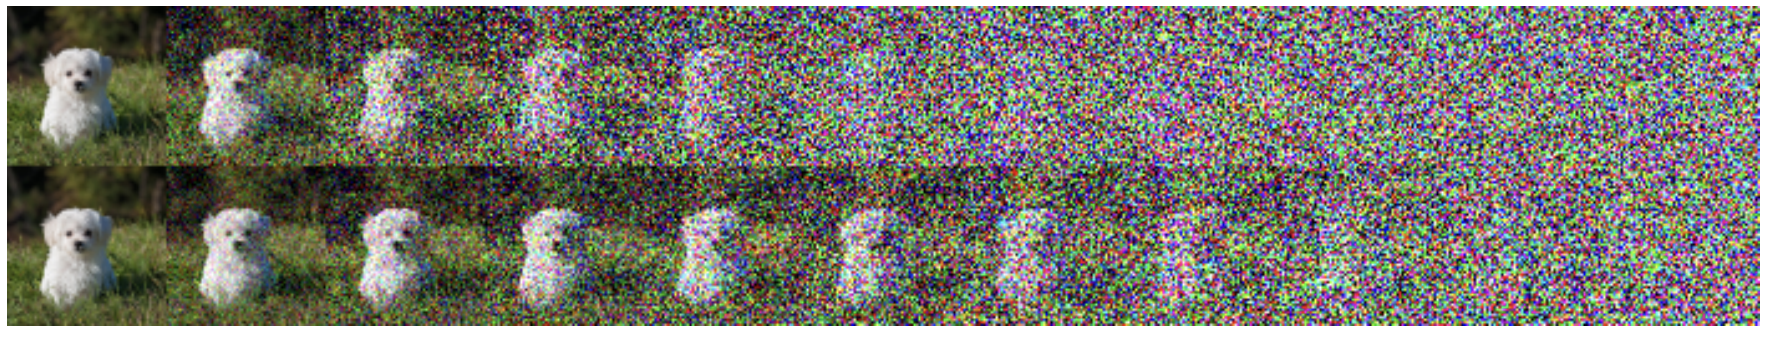
\includegraphics[width=1\textwidth]{images/diffusion_models/linear_cosine_scheduler.png}
    \caption{Linear scheduler (top, \cite{ddpm}) and cosine scheduler (bottom, \cite{openai_improved_ddpm}) shows that linear scheduler adds noise too quickly which degrades the model's performance whereas cosine scheduler adds noise more slowly.}
    \label{fig:linear_cosine_scheduler}
\end{figure}







\subsection{Encoder}

The forward diffusion process maps a data image $x$ through a series of intermediate variables $z_1, ..., z_T$ with the dimension as $x$ according to the following recursion:

\begin{equation}
    \begin{aligned}
    \mathbf{z}_1 &= \sqrt{1 - \beta_1} \cdot \mathbf{x} + \sqrt{\beta_1} \cdot \epsilon_1, \\
    &\;\;\vdots \notag \\
    \mathbf{z}_t &= \sqrt{1 - \beta_t} \cdot \mathbf{z}_{t-1} + \sqrt{\beta_t} \cdot \epsilon_t \quad \forall \, t \in \{2, \ldots, T\}
    \end{aligned}
\end{equation}

At each step $i \in {1, 2, ..., t, t+1, ..., T}$ a noise vector $e_i$ is drawn from a standard normal distribution. This equation adds random noise $e_i$ to the data (image) $x = z_0$ and $\beta$ is a schedule function ($\beta(t):[1, ..., T] \rightarrow \mathbb{R}$) that determines the amount of noise added at each step ($\beta$ is a variance schedule, which can be linear, cosine, quadratic and more). 

A more formal notation for the forward process is:

\begin{equation*}
    \begin{aligned}
        q(x_t | x_{t-1}) = \mathcal{N}(x_t; \sqrt{1-\beta_t} \cdot x_{t-1}, \beta_t \mathbf{I}) \\
        q(x_{1:T} | x_0) = \prod_{t=1}^{T} q(x_t | x_{t-1})
    \end{aligned}
\end{equation*}

In the above formula we can see that to define the next timestep $x_t$ and to get a noisier image, we define it as gaussian / normal distribution where the mean is $\sqrt{1-\beta_t} x_{t-1}$ and variance $\beta_t \mathbf{I}$. The $\beta$ parameter is the noise scheduler (how much noise we add at each step). This process is known as Markov Chain, since the next step depends only on the previous step (see appendix \ref{appendix:markov_chains}).

An interesting point the authors made is that its possible to sample $x_t$ from any arbitrary timestep $t$, given the original image $x_0$ (without calculating all the intermediate steps):

\begin{equation}
    \begin{aligned}
    q(\mathbf{x}_t|\mathbf{x}_0) = \mathcal{N}(\mathbf{x}_t; \sqrt{\bar{\alpha}_t}\mathbf{x}_0, (1 - \bar{\alpha}_t)\mathbf{I}) \\
    \text{where } \alpha_t := 1 - \beta_t \text{ and } \bar{\alpha}_t := \prod_{i=1}^{t} \alpha_i
    \end{aligned}
    \label{eq:forward_diffusion}
\end{equation}

Equation \ref{eq:forward_diffusion} describes the process of adding noise, $x_t$ from $x_0$ without any intermediate steps.

Since $\alpha$ depends on $\beta$ and $\beta$ is a noise scheduler (fixed), there are no parameters to learn in the forward process.

Each diffusion model has slightly different implementation in its network, and this encoder formulation generalizes the encoder process. We will take a closer look on the encoder/decoder network in the Stable Diffusion paper \cite{stable_diffusion} in the next section \ref{sec:stable_diffusion} and its code implementation.










\subsection{Decoder}

The decoder removes noise from the intermediate latent variables $z_1, ..., z_T$ and reconstructs the original image $x$ using the following recursion:

\begin{equation}
    p_\theta(\mathbf{x}_{t-1} | \mathbf{x}_t) = \mathcal{N}(\mathbf{x}_{t-1}; \mu_\theta(\mathbf{x}_t, t), \Sigma_\theta(\mathbf{x}_t, t))
    \label{eq:reverse_diffusion}
\end{equation}

where $\theta$ are the learned parameters of the model. The mean $\mu_\theta$ and variance $\Sigma_\theta$ are unknown and should be learned in the training stage. However, in the DDPM paper \cite{ddpm} the auhtors said:

\begin{quote}
    \textit{"We also see that learning reverse process variances (by incorporating a parameterized diagonal $\Sigma_\theta(x_t)$ into the variational bound) leads to unstable training and poorer sample quality compared to fixed variances."} \cite{ddpm}
\end{quote}

The OpenAI team released a paper titled "Improved denoising diffusion probabilistic models" \cite{openai_improved_ddpm} in which the authors used cosine noise (instead of linear in the original paper \cite{ddpm}) scheduler and also learned the variance, which significantly improved the model's performance.








\subsection{Loss function}

The loss function of DDPMs is typically the ELBO loss function (negative log-likelihood \ref{eq:elbo}):

\begin{equation*}
    \mathbb{E}[-\log p_\theta (x_0)] \leq \mathbb{E}_q[-\log \frac{p_\theta(x_{0:T})}{q(x_{1:T}|x_0)}] = \mathcal{L}
\end{equation*}

The left term is the negative log likielihood. The upper bound is the tractable ELBO loss function. The dominator $q(x_{1:T}|x_0)$ is the forward diffusion process (adds noise) and the numerator $p_\theta(x_{0:T})$ is the model's joint distribution over latent steps $x_1, ..., x_T$ which is the reverse process. The ratio of these two terms is the ELBO loss function, when this ratio reaches 1 it indicates that the model can undo the forward process. We also don't write $q_\theta$ because the forward process is not learned, only the reverse process is leanred.

Like we discussed before, diffusion models are latent variable models in the form of $p_\theta (x_0) := \int p_\theta(x_{0:T}) d\mathbf{x}_{1:T}$ which is intractable. Which is why we use the ELBO loss function to approximate the likelihood of the data (see appendix \ref{appendix:elbo}).






\subsection{Training}

The training of diffusion models is done by sampling a batch of images from the dataset, and then adding noise to the images in the forward diffusion process. The model is trained to remove the noise and reconstruct the original image in the reverse diffusion process. The loss function is the ELBO loss function (see previous section). Usually, the model is trained using stochastic gradient descent (SGD), but more advanced optimizers like Adam can be used as well.

\begin{figure}
    \centering
    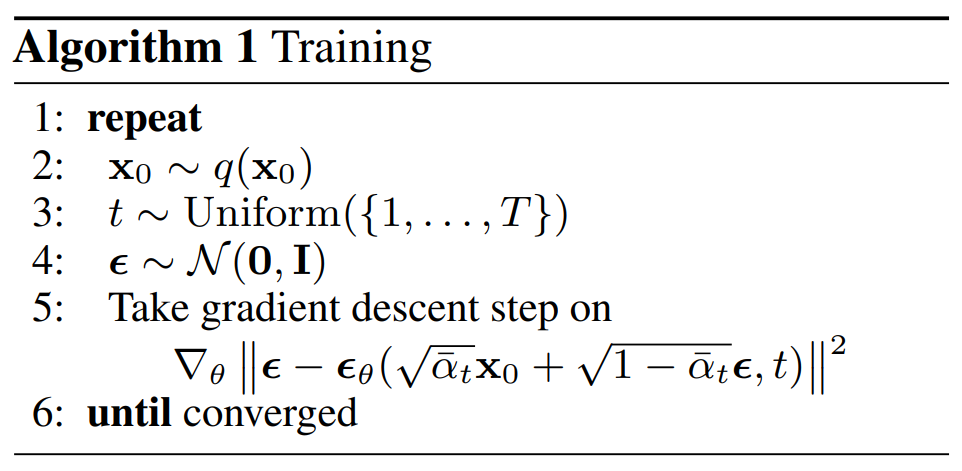
\includegraphics[width=0.5\textwidth]{images/diffusion_models/training.png}
    \caption{The training algorithm of diffusion models \cite{ddpm}. Line 2: we take a sample from the dataset. Line 3: we generate random number between 1 and T uniformly. Line 4: we sample some noise. Line 5: we calculate the gradients of the loss function.}
    \label{fig:ddpm_training}
\end{figure}

In figure \ref{fig:ddpm_training} line 5, we try to optimize the model's parameters $\theta$ by gradient decent. $\epsilon_\theta$ is the predicted noise added at timestep $t$ (a function approximator with 2 parameters that intends to predict $\epsilon$ from $x_t$) where the first parameter is the noisy image at timestep $t$, and the second parameter is the timestep ($t$). 








\section{Stable Diffusion}
\label{sec:stable_diffusion}


\begin{figure}
    \centering
    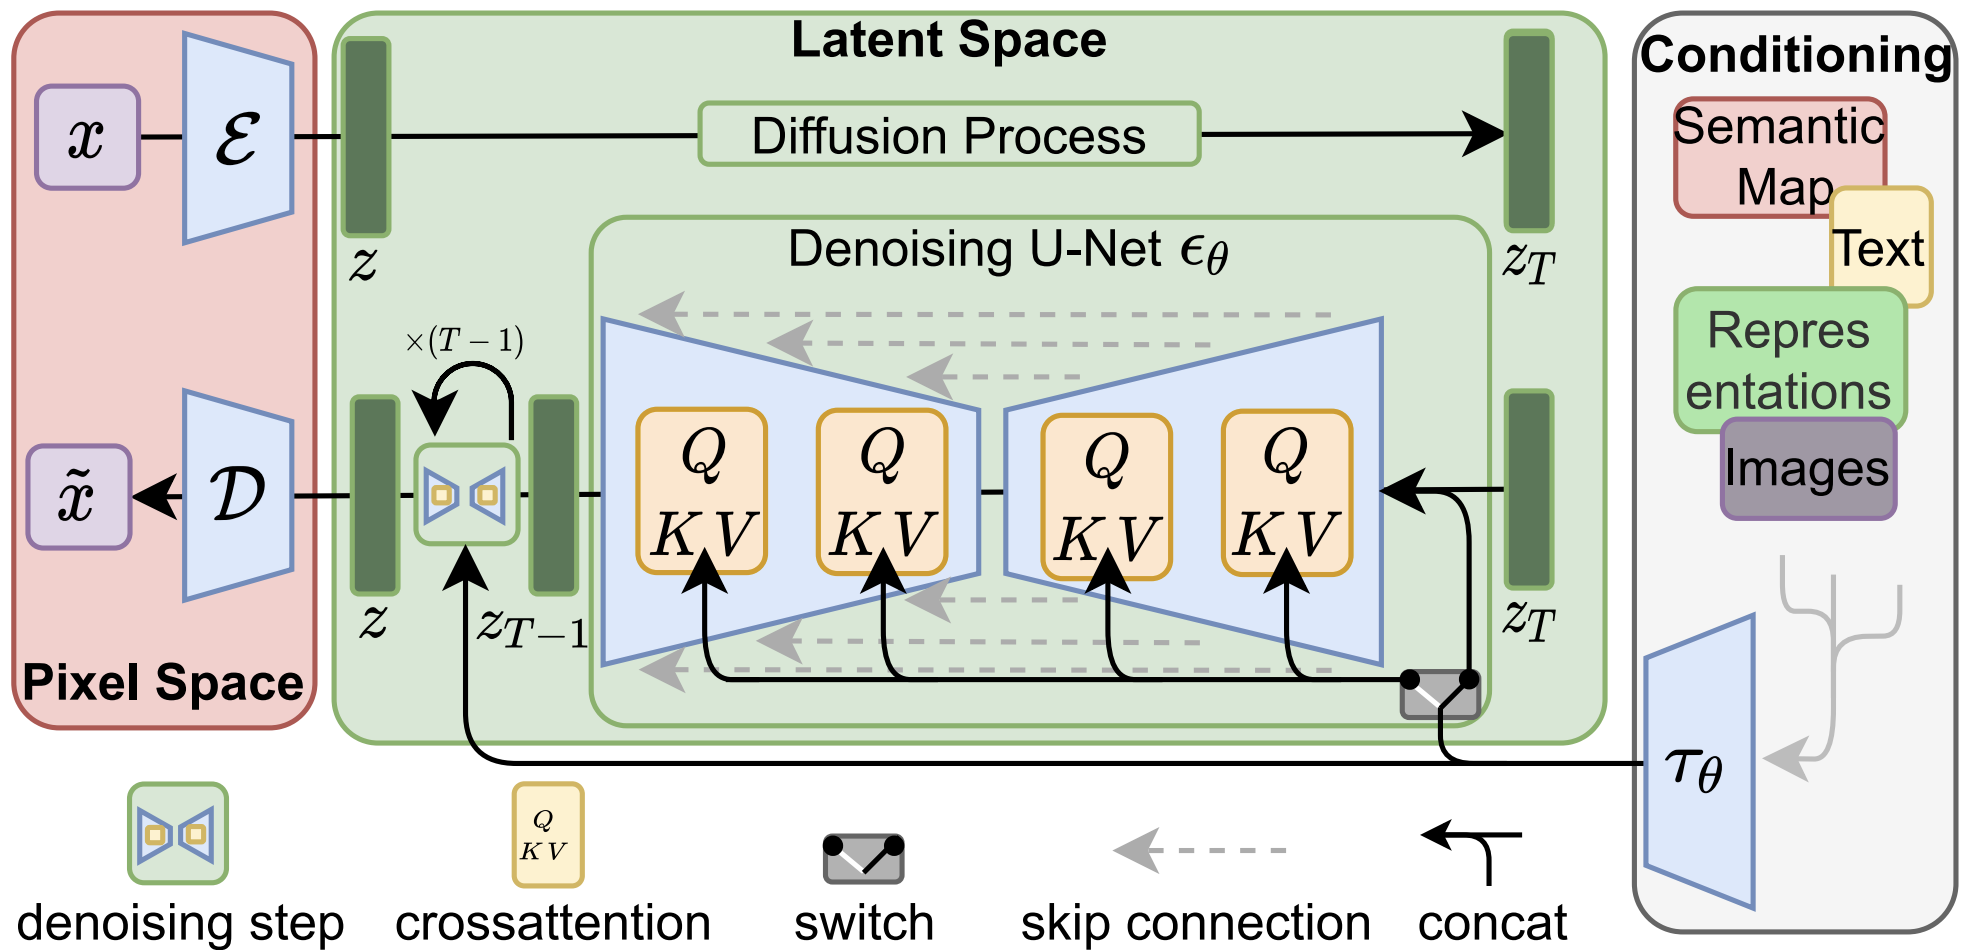
\includegraphics[width=0.6\textwidth]{images/diffusion_models/stable_diffusion/stable_diffusion.png}
    \caption{Stable diffusion scales better compared to other models \cite{stable_diffusion} (DALL-E, VQ-GAN) with less downsampling blocks ($f = 4$ instead of 16 as needed by VQ-GAN).}
\end{figure}


In the Stable Diffusion paper \cite{stable_diffusion} the authors suggested that computing gradients directly in DDPMs on the pixel space is inefficient, since this space is highly-dimensional and includes undesired high-frequency details. They suggest to convert the input images to a lower-dimensional latent representations and then apply the diffusion processes. The authors showed that this approach \textbf{scales better} and is more compute efficient \footnote{In the Stable Diffusion paper \cite{stable_diffusion} the authors showed that the model can be trained on a single GPU with 16GB of memory on images of $256\times 256$ resolution using CelebA-HQ dataset with 30 diffusion steps.} compared to working in pixel space. Moreover, the authors introduced general purpose \textbf{conditioning mechanism based on cross-attention} which allows multi-modal training.

A 2021 paper released by OpenAI \cite{openai_diffusion_beats_gans} shows that \textbf{diffusion models can outperform GANs} in terms of image fidelity by trading off diversity.











\subsection{The U-Net backbone}
\label{subsec:stable_diffusion_u_net_backbone}

U-Net (first introduced in 2015) \cite{unet} is a convolutional neural network (CNN) architecture that is commonly used in diffusion models. U-Net is used as a backbone for denoising the latent variables $z_1, ..., z_T$. The U-Net architecture is a symmetric encoder-decoder network with skip connections between the encoder and decoder: the skip connections help the network to learn better by minimizing the \textbf{exploding / vanishing gradient problems} \cite{exploding_vanishing_gradients}.

\begin{figure}
    \centering
    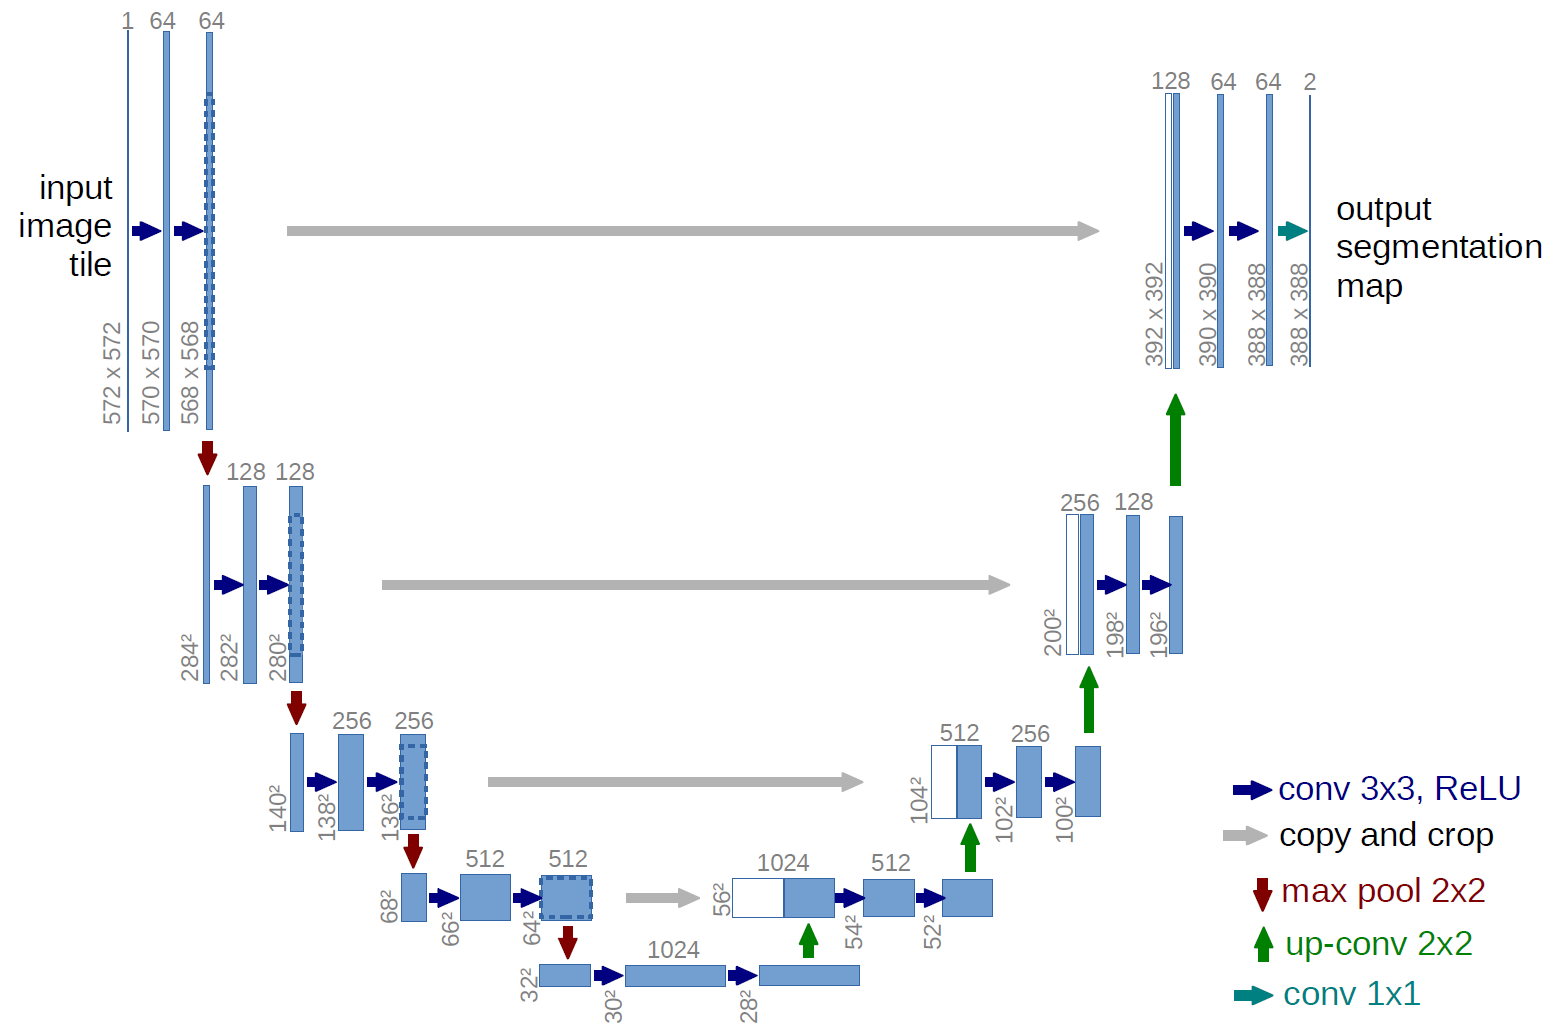
\includegraphics[width=0.5\textwidth]{images/diffusion_models/stable_diffusion/u-net-architecture.png}
    \caption{The U-Net architecture \cite{unet} with convolutional and deconvolutional layers \& skip connections.}
    \label{fig:unet_architecture}
\end{figure}

In figure \ref{fig:unet_architecture} the U-Net is shaped like a 'U' in which the input is downsampled to low spatial resolution and high feature channels and then upsampled back again. The convolution kernel size is 3x3 and they use ReLU activation function.








\subsection{Sinusoidal embeddings}
\label{subsec:sinusoidal_embeddings}

The diffusion process uses \textbf{timestep embeddings} which is a scalar representing the current diffusion timestep: $t \in [0, T]$. This way the model knows if its in the beginning of the diffusion or at the late stage, which is essential for removing noise. 

To get the embeddings, the timestep is first projected into a \textbf{sinusoidal embedding}, similar to the way positional encodings are used in transformers.

\begin{figure}[h]
    \centering
    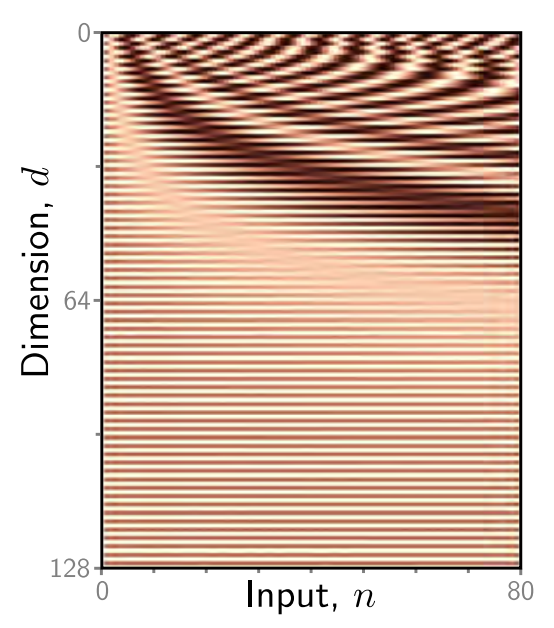
\includegraphics[width=0.25\textwidth]{images/diffusion_models/stable_diffusion/positional_encodings.png}
    \caption{Sinusoidal positional embeddings used in a transformers \cite{understanding_deep_learning_book_2024}. \textit{X axis}: the input scalar (position in a transformer or timestep in diffusion model). \textit{Y axis}: the embeddings dimensions \cite{understanding_deep_learning_book_2024}.}
    \label{fig:sinusoidal_embeddings}
\end{figure}

In figure \ref{fig:sinusoidal_embeddings} we can see the sinusoidal positional embeddings used in a transformer model, which is similar to timestep embeddings. The pattern is sinusoidal where lighter regions indicate lower values and darker regions indicate higher values. Each column in the X axis is a \textbf{unique embedding}. For example, the scalar '1' will have different encodings than a scalar '2', which helps distinguish the position / timestep of the input sequence.

\begin{lstlisting}[language=Python, breaklines=true, caption={Timestep embeddings in Stable Diffusion: we convert the timestep to an embedding.}, label={lst:timestep_embeddings_stable_diffusion}]
def get_time_embedding(timestep):
    # Shape: (160,)
    freqs = torch.pow(10000, -torch.arange(start=0, end=160, dtype=torch.float32) / 160) 
    # Shape: (1, 160)
    x = torch.tensor([timestep], dtype=torch.float32)[:, None] * freqs[None]
    # Shape: (1, 160 * 2)
    return torch.cat([torch.cos(x), torch.sin(x)], dim=-1)
\end{lstlisting}

The general formula for timestep embeddings is given in equation \ref{eq:timestep_embeddings}. The code snippet in listing \ref{lst:timestep_embeddings_stable_diffusion} is taken from \href{https://github.com/hkproj/pytorch-stable-diffusion/blob/e0cb06de011787cdf13eed7b4287ad8410491149/sd/pipeline.py#L164}{a re-implementation of Stable Diffusion}.

\begin{equation}
    \text{Enc}_i(t) =
    \begin{cases}
        \sin\left(\frac{t}{10000^{\frac{2i}{d}}}\right) & \text{if } i \text{ is even} \\
        \cos\left(\frac{t}{10000^{\frac{2i}{d}}}\right) & \text{if } i \text{ is odd}
    \end{cases}
    \label{eq:timestep_embeddings}
\end{equation}










\subsection{Architecture}

\begin{figure}
    \centering
    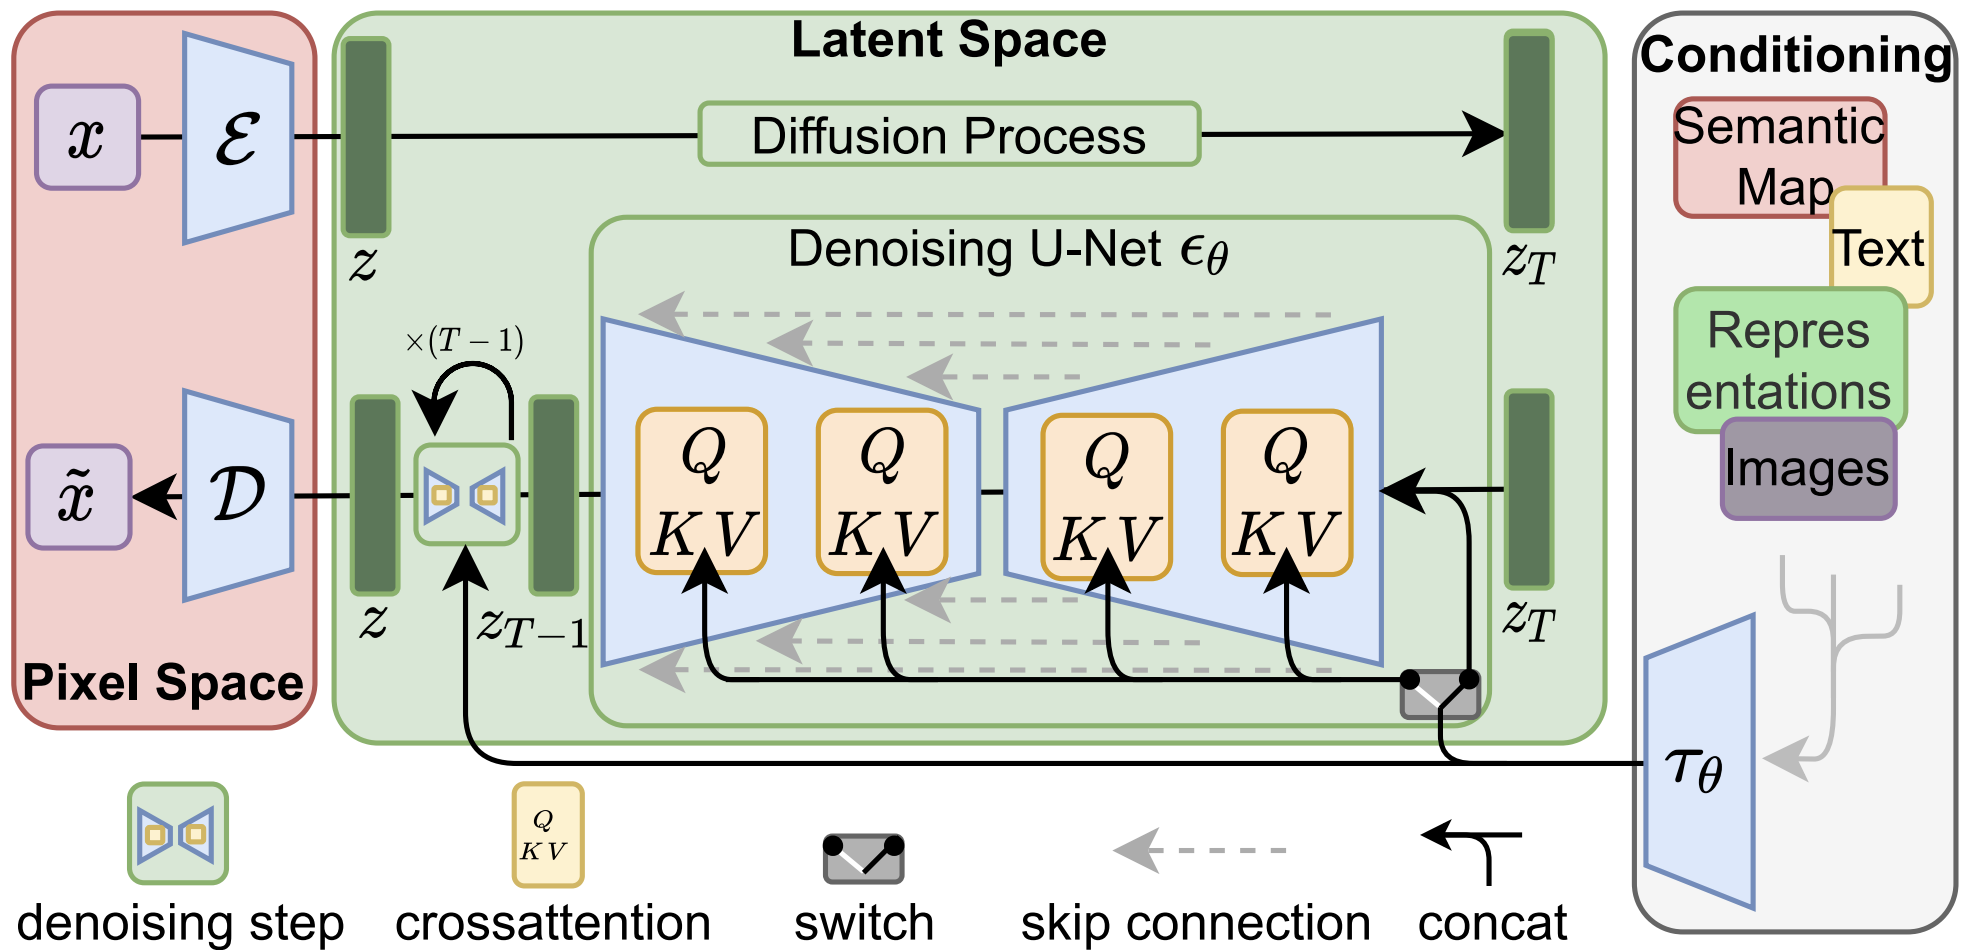
\includegraphics[width=0.5\textwidth]{images/diffusion_models/stable_diffusion/architecture.png}
    \caption{Stable Diffusion architecture \cite{stable_diffusion}.}
    \label{fig:stable_diffusion_architecture}
\end{figure}

The high-level architecture is shown in figure \ref{fig:stable_diffusion_architecture}. The stable diffusion model, which is a latent diffusion model (LDM), consists of: 

\begin{itemize}
    \item Variational autoencoder (VAE) which compresses the input images into regularized latent space. It consists of:
    \begin{itemize}
        \item Encoder $\varepsilon$ which converts the input images $x$ to latent space $z$.
        \item Decoder $\mathcal{D}$ which converts the latent vector $z$ back to the pixel space $\tilde{x}$.
    \end{itemize}
    \item A U-Net backbone which which serves as the noise prediction network, predicts the noise needed to denoise the intermediate latent vectors $z_T, ..., z_1$ in each step. It incorporates timestep embeddings as an essential input.
    \item A domain specific encoder $\tau_\theta$ which encodes the conditional information (text prompts, images, segmentation masks) into tokens which will be used in the cross-attention layers, or concatenated with the latent vector (the switch mechanism).
\end{itemize}







\subsection{Conditioning}

Cross-attention (appendix \ref{appendix:attention}) is used in Stable Diffusion for \textbf{multi-modal conditioning}: it guides the model to output images based on conditional information. Although this information is multi-modal (e.g. images, text, segmentation masks), the cross-attention layers in the U-Net and the switch mechanism able to process them all.

\textbf{Text conditioning}: if the conditioning signal is text prompt, the domain specific encoder $\tau_\theta$ is a text encoder (tokenizer) which converts the text words to embeddings (tokens). In the paper \cite{stable_diffusion} the authors used a \href{https://github.com/CompVis/latent-diffusion/blob/a506df5756472e2ebaf9078affdde2c4f1502cd4/ldm/modules/encoders/modules.py#L138}{\textbf{frozen CLIPTokenizer}}, which is a pre-trained tokenizer trained on specific vocabulary, and special tokens (beginning of sentence, end of sentence, padding, mask tokens and more). However, digging into the source code, you will find other text encoders as well such as \href{https://github.com/CompVis/latent-diffusion/blame/a506df5756472e2ebaf9078affdde2c4f1502cd4/ldm/modules/encoders/modules.py#L53}{\textbf{BERT}} \cite{bert}.

\textbf{Switch mechanism}: In figure \ref{fig:stable_diffusion_architecture} the 'switch' in the diagram is used for different kinds of conditional information. If the conditional information is spatial (such as images, layouts, semantic masks), they use concatenation with $z_T$. In the case of text (not spatial), they use cross-attention layers. 

We dive deeper into self-attention, multi-head attention and cross-attention in the appendix \ref{appendix:attention}, which are commonly used in other image and video synthesis models.













\subsection{Classifier-free diffusion guidance (CFG)}

\label{subsec:classifier_free_diffusion_guidance}

Classifier-free guidance (CFG) (see section \ref{subsec:classifier_free_diffusion_guidance}) is used in Stable Diffusion to control the influence of the conditioning signal and balance between being faithful to the conditioning signal or being diverse in the generated samples.

So far we have focused on modeling just the data distribution $p(x)$. However, we are often also interested in learning conditional distribution $p(x|y)$, which would enable us to explicitly control the data we generate through conditioning signal $y$.

We can add conditioning information alongside the timestep information, at each iteration:

\[
p(x_{0:T}) = p(x_T) \prod_{t=1}^{T} p_\theta (x_{t-1} | x_{t, y})
\]

When training a diffusion model to generate images based on specific conditional information, there's a risk that the model might not fully consider or even ignore these conditions, using this vanilla formulation. To address this, a technique called "guidance" is used. Guidance allows us to explicitly control \textbf{how much influence the conditions have on the generated images}, but this can sometimes lead to less variety in the results. In other words, we use weight to control how much the model should pay attention to the conditioning signal.


Conditioning a generative model can be achieved through two methods: 

\begin{itemize}
    \item classifier guidance
    \item and classifier-free guidance.
\end{itemize}





\subsubsection*{Classifier guidance}

Classifier guidance \cite{openai_diffusion_beats_gans} involves \textbf{training a separate model} to condition the output, and is based on score-based diffusion models \cite{score_based_generative_modeling}. 

Classifier guidance formulation is given as:

\[
\nabla \log p(x_t | y) = \underbrace{\nabla \log p(x_t)}_{\text{unconditional score}} + \underbrace{\gamma \nabla \log p(y | x_t)}_{\text{adversarial gradient}}
\]

where $\gamma$ is a hyperparameter that controls the strength of the conditioning signal in classifier guidance method.








\subsubsection*{Classifier-free guidance}

In Classifier-free guidance (CFG) \cite{classifier_free_guidance}, instead of training two networks, one conditional network and an unconditional network, we train a single network, and during training, \textbf{we set the conditioning signal to zero} with some probability. This way, the network becomes a mix of conditioned and unconditioned networks, and we can take the conditioned and unconditioned output and combine them with weight that indicates how much we want the network to pay attention to the conditioning signal. 

The formulation for classifier-free guidance is given by:

\[
\nabla \log p(x_t | y) = \underbrace{\gamma \nabla \log p(x_t | y)}_{\text{conditional score}} + \underbrace{(1 - \gamma) \nabla \log p(x_t)}_{\text{unconditional score}}
\]

In contrast to classifier guidance, classifier-free guidance streamlines the training process and lowers computational costs by utilizing a single model instead of training two separate models.

\begin{lstlisting}[language=Python, caption={Classifier-free guidance (CFG) in Stable Diffusion.}, label={lst:cfg_stable_diffusion}]
if do_cfg:
    output_cond, output_uncond = model_output.chunk(2)
    model_output = cfg_scale * (output_cond - output_uncond) + output_uncond
\end{lstlisting}

In listing \ref{lst:cfg_stable_diffusion} the code snippet is taken from \href{https://github.com/hkproj/pytorch-stable-diffusion/blob/e0cb06de011787cdf13eed7b4287ad8410491149/sd/pipeline.py#L135C1-L136C1}{a re-implementation of Stable Diffusion}, but the official implementation of Stable Diffusion is \href{https://github.com/CompVis/stable-diffusion/blob/21f890f9da3cfbeaba8e2ac3c425ee9e998d5229/ldm/models/diffusion/ddim.py#L178C1-L179C1}{very similar}.

















\subsection{Contrastive Language Image Pre-training (CLIP)}
\label{subsec:clip}

In Stable Diffusion, the authors used CLIP as the text encoder for the conditional text prompts.

CLIP (Contrastive Language Image Pre-training) \cite{openai_clip} is a model developed by OpenAI that learns visual concepts from text supervision. The model builds \textbf{associations between images and text prompts}. Often this association is called 'text-image alignment', or 'image-text alignment'. It models how well a generated image corresponds to its associated text description.

The \textbf{CLIPTokenizer}, which is part of the CLIP model, converts text prompts to a sequence of tokens which are then used in the latent space of the Stable Diffusion model.

\begin{figure}
    \centering
    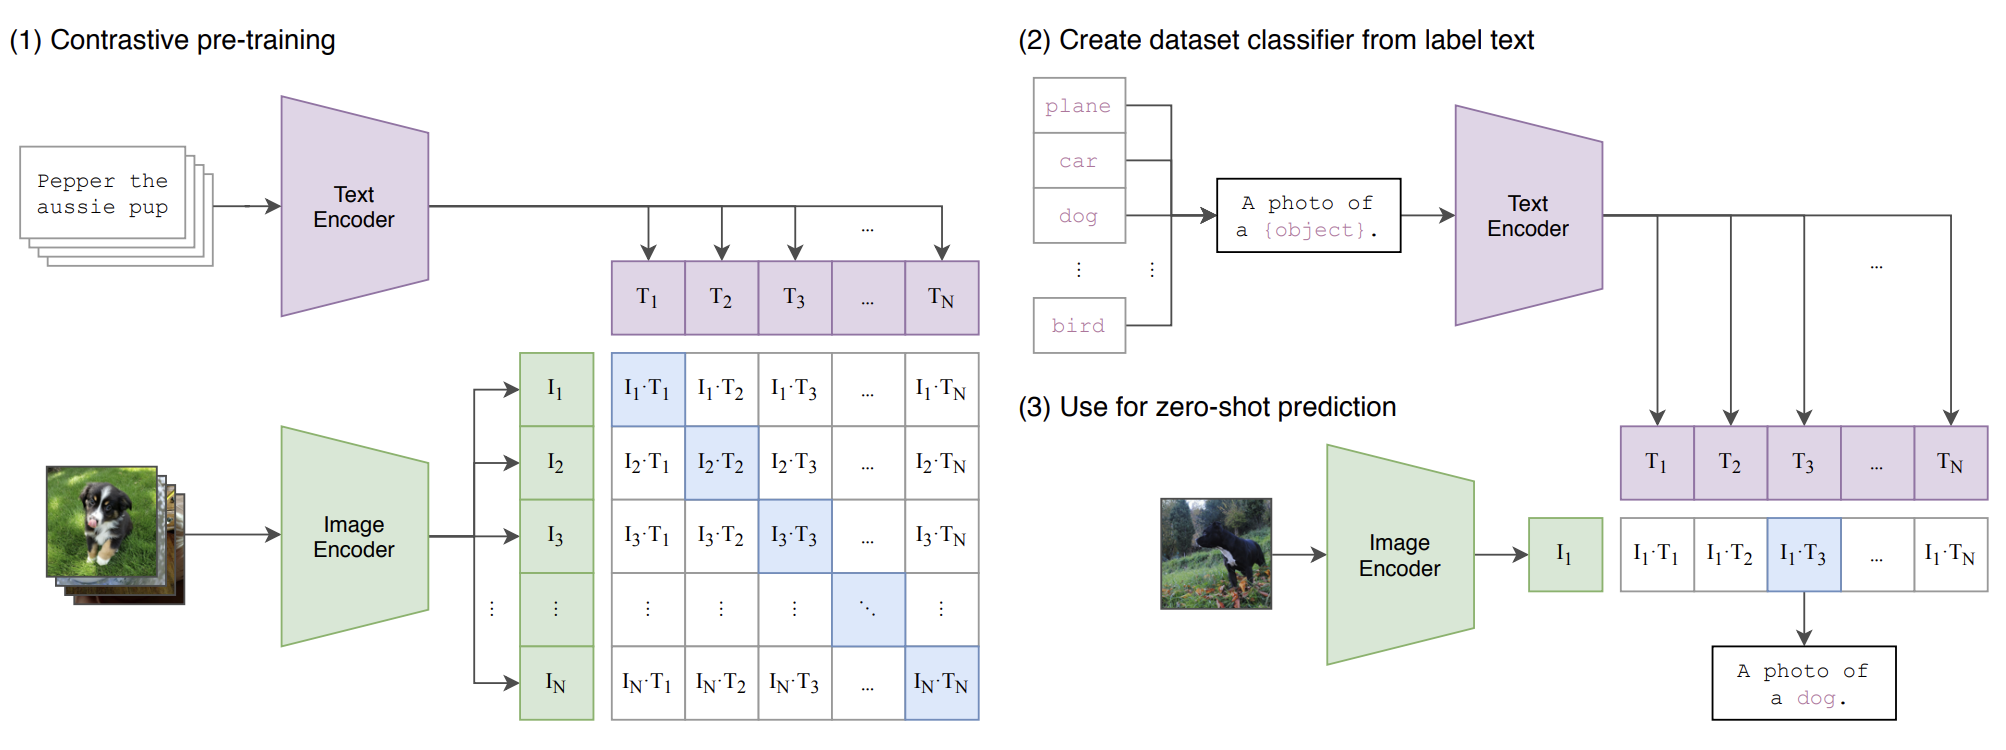
\includegraphics[width=0.7\textwidth]{images/diffusion_models/stable_diffusion/clip.png}
    \caption{(1) Contrastive pre-training stage of a CLIP model (training stage). (2) and (3): after the model has been pre-trained, its used as a zero-shot image classifier \cite{openai_clip}.}
    \label{fig:openai_clip}
\end{figure}

In figure \ref{fig:openai_clip},  $I_1, ..., I_N$ are the images, and $T_1, ..., T_N$ are the text prompts. The output is a \textbf{matrix of similarity scores} between the images and the text descriptions. Ideally in the matrix diagonal we get high similarity score (1) indicating high text-image alignment, and all other entries ideally should have low similarity score (0), indicating mismatch in text-image alignment.

The CLIP network is compromised of:

\begin{itemize}
    \item \textbf{Image encoder}: converts images to image embeddings.Its typically a vision transformer (ViT) \cite{vision_transformer} (appendix \ref{appendix:vision_transformer}) or a ResNet \cite{resnet} model.
    \item \textbf{Text encoder}: converts text descriptions to text embeddings. Its typically implemented as a transformer, or less common as a continuous bag of words \cite{cbow_word2vec} (known as Word2Vec model by Google, 2013 \cite{cbow_word2vec}).
    \item \textbf{Training objective}: the CLIP model is trained using a contrastive objective (commonly referred to as CLIP objective), where the goal is to minimize the cosine distance in the main diagonal and maximize the distance for non-matching image-text pairs (off diagonal).
\end{itemize}





















\subsection{DDIM Sampler}
\label{subsec:ddim_sampler}

\begin{figure}[ht]
    \centering
    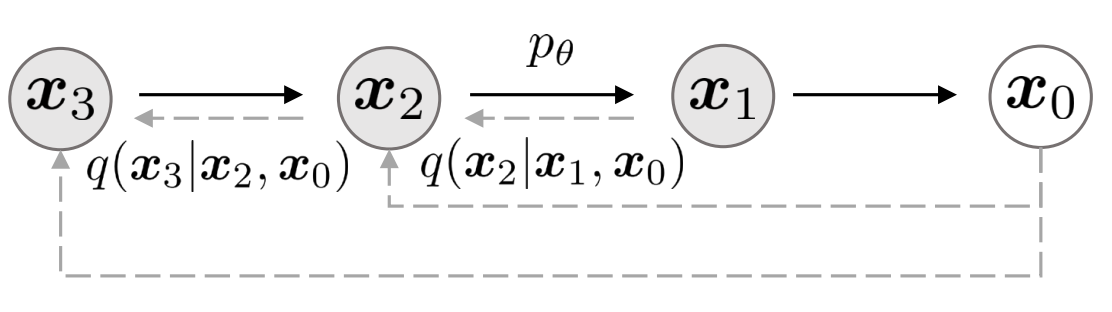
\includegraphics[width=0.4\textwidth]{images/diffusion_models/stable_diffusion/ddim_non_markov_process.png}
    \caption{Non-Markovian inference in DDIM. Each step depends on both the previous step and the initial state $x_0$ \cite{ddim}.}
    \label{fig:ddim_non_markov_process}
\end{figure}

Denoising Diffusion Implicit Models (DDIM), introduced in \cite{ddim}, provide an \textbf{efficient sampling method} for diffusion models, offering improvements over the traditional Denoising Diffusion Probabilistic Models (DDPM) \cite{ddpm}. Unlike DDPM sampler, which uses a fixed noise schedule and stochastic sampling, DDIM introduces a flexible noise schedule and a \textbf{deterministic sampling process}, enabling faster inference (10x to 50x speedup compared to DDPM \cite{ddim}).

Key points \& main contributions of the DDIM paper:

\begin{itemize}
    \item \textbf{Non-Markovian process}: As illustrated in figure \ref{fig:ddim_non_markov_process}, DDIM's reverse process depends on both the previous step and the initial state $x_0$, forming a deterministic trajectory through the latent space.
    \item \textbf{Implicit probabilistic model}: DDIM is an implicit probabilistic model, meaning that it doesn't directly model the joint distribution of the data but rather models the conditional distribution of the data given the noise.
    \item \textbf{Deterministic sampling}: Noise is removed directly in a controlled manner, skipping unnecessary diffusion steps and avoiding stochasticity.
    \item \textbf{Training objective}: DDIM uses the same training objective as DDPM and no modifications are needed.
    \item \textbf{Sampling process}: Sampling in DDIM involves sampling from the prior distribution and then iteratively sampling from the conditional distributions. This process is faster than traditional diffusion models because it doesn't require simulating the entire Markov chain.
\end{itemize}

DDIM introduces a generalized forward process:

\[
q_\sigma (x_{t-1} | x_t, x_0) = \mathcal{N} \left( \sqrt{\alpha_{t-1}} x_0 + \sqrt{1 - \alpha_{t-1} - \sigma_t^2} \cdot \frac{x_t - \sqrt{\alpha_t} x_0}{\sqrt{1 - \alpha_t}}, \sigma_t^2 I \right),
\]

where $\sigma \in \mathbb{R}^T_{\geq 0}$ controls the stochasticity of the forward process:
- For $\sigma \rightarrow 0$, the process becomes fully deterministic, as $x_{t-1}$ is uniquely determined by $x_t$ and $x_0$.

\begin{figure}
    \centering
    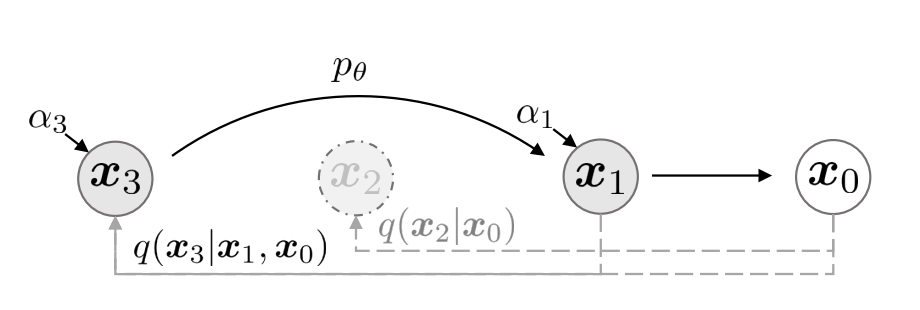
\includegraphics[width=0.5\textwidth]{images/diffusion_models/stable_diffusion/ddim_sampling_process.png}
    \caption{DDIM sampling \cite{ddim}. In the figure, $x_3$ depends only on $x_0$ and $x_1$ (and not $x_2$). This process can be generalized to all subsets of steps.}
    \label{fig:ddim_sampling_process}
\end{figure}

\begin{figure}
    \centering
    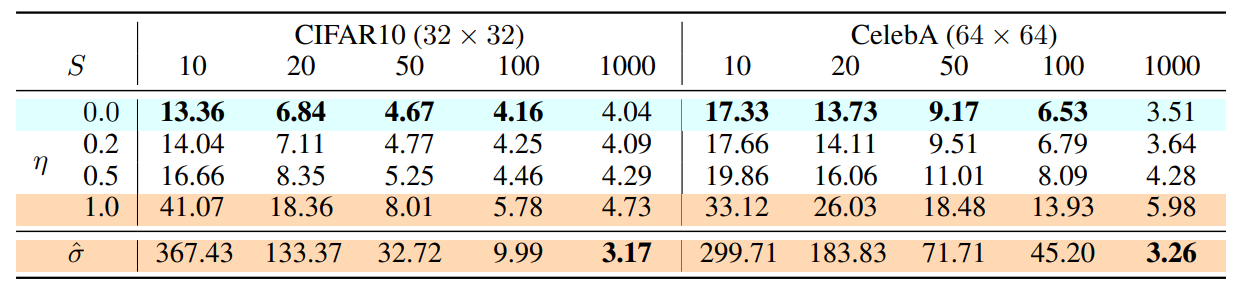
\includegraphics[width=0.7\textwidth]{images/diffusion_models/stable_diffusion/ddim_sample_quality.png}
    \caption{DDIM gives almost the same sample quality compared to DDPM sampler, and requires less compute since we skip some of the diffusion steps. The stochasticity of the model is controlled by $\eta$ \cite{ddim}.}
    \label{fig:ddim_sample_quality}
\end{figure}

In figure \ref{fig:ddim_sample_quality} DDIM gives almost the same sample quality in FID metric (equation \ref{eq:fid_score}, lower is better) compared to DDPM and require much less compute. The experiment was done on CIFAR10 and CelebA datasets, with 10,20,50,100,1000 steps. When $\eta = 0$ (blue) the model is deterministic (DDIM process), and when $\eta = 1$ (orange) the model is stochastic (DDPM process).















\subsection{Training}

Stable Diffusion is trained in CFG manner (section \ref{subsec:classifier_free_diffusion_guidance}).

The authors made simplified loss objective which predicts the noise removal process at each step:

\[
    L_{\text{DM}} = \mathbb{E}_{x, \epsilon \sim \mathcal{N} (0, 1), t} \left[ \Vert \epsilon - \epsilon_\theta(x_t, t) \Vert _2^2 \right]
\]

This loss function is similar to the loss function of DDPM (equation \ref{eq:ddpm_loss}).













\subsection{Implementation of $\tau_\theta$ transformer for conditional LDMs}

The researchers provded high level overview of the implementation of the conditional encoder for text $\tau_\theta$, consisted of $N$ transformer blocks:

\begin{align*}
    &\zeta \leftarrow \text{TokEmb}(y) + \text{PosEmb}(y) \\
    &\text{for } i = 1, \ldots, N : \\
        &\hspace{1cm} \zeta_1 \leftarrow \text{LayerNorm}(\zeta) \\
        &\hspace{1cm} \zeta_2 \leftarrow \text{MultiHeadSelfAttention}(\zeta_1) + \zeta \\
        &\hspace{1cm} \zeta_3 \leftarrow \text{LayerNorm}(\zeta_2) \\
        &\hspace{1cm} \zeta \leftarrow \text{MLP}(\zeta_3) + \zeta_2 \\
    &\zeta \leftarrow \text{LayerNorm}(\zeta)
\end{align*}

where:

\begin{itemize}
    \item $\zeta := \tau_\theta(y)$ is the unmasked transformer output (the transformer processes the tokenized version of $y$), which is then used in the cross-attention mechanism of the stable diffusion model.
    \item TokEmb is the token embeddings.
    \item PosEmb is the positional embeddings.
    \item LayerNorm is the layer normalization (appendix \ref{appendix:blocks_norm}).
    \item MultiHeadSelfAttention is the multi-head self-attention mechanism (appendix \ref{appendix:attention}).
    \item and MLP is the multi-layer perceptron (appendix \ref{appendix:blocks}) block.
\end{itemize}


\begin{figure}[h]
    \centering
    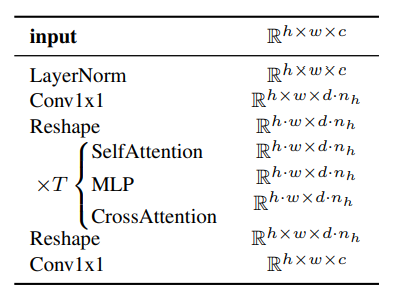
\includegraphics[width=0.3\textwidth]{images/diffusion_models/stable_diffusion/transformer_block.png}
    \caption{Architecture of the transformer block used in Stable Diffusion, where $n_h$ denotes the number of attention heads and $d$ the dimensionality per head \cite{stable_diffusion}.}
\end{figure}











\subsection{Details on Autoencoders Models}

In the stable diffusion paper, the researchers trained the pixel-space encoder $\varepsilon$ and the decoder $\mathcal{D}$ in adversarial manner (adversarial loss \cite{vqgan}). A patch-based discriminator $D_\psi$ is optimized to differentiate the original image from reconstructed image $\mathcal{D} (\varepsilon (x))$ which helps guide the autoencoder.

In addition, the researchers used two methods for regularizing the latent space:

\begin{itemize}
    \item \textbf{KL-divergence regularization}: similar to VAEs where the latent space is a distribution, the KL regularization objective pushes the latent space to be close to a standard normal distribution.
    \item \textbf{VQ regularization}: similar to VQ-GAN and VQ-VAE (sections \ref{vqgan} and \ref{vqvae}), the vector quantization regularization forces the latent space to be discrete, which can help the model to learn better by using a codebook $\mathcal{Z}$.
\end{itemize}

They factorized the KL term by a factor of $\sim 10^{-6}$, and in VQ regularization they used a big codebook.

The full loss objective to train the autoencoder model $(\varepsilon, \mathcal{D})$ is given by:

\begin{equation*}
    L_{\text{Autoencoder}} = \min_{\varepsilon, \mathcal{D}} \max_{\psi} \left( L_{\text{rec}} (x, \mathcal{D} (\varepsilon (x))) - L_{\text{adv}} (\mathcal{D} \varepsilon (x)) + \log \mathcal{D}_\psi (x) + L_{\text{reg}} (x; \varepsilon, \mathcal{D}) \right)
\end{equation*}


















\subsection{Experiments}

The researchers conducted several experiments with different LDM downsampling factors, and compared the results with other state-of-the-art models (DALL-E, VQGAN, StyleGAN, ProjectedGAN, CogView, GLIDE, and others).

\begin{figure}
    \centering
    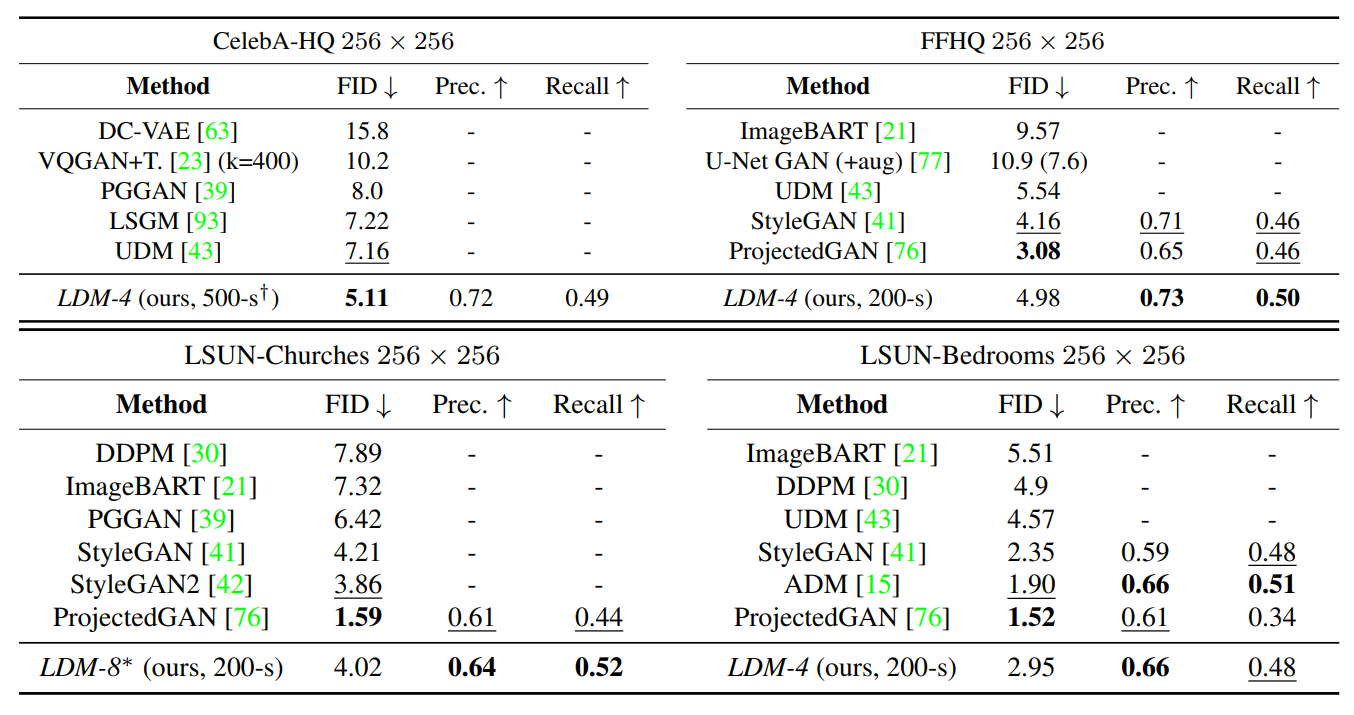
\includegraphics[width=0.7\textwidth]{images/diffusion_models/stable_diffusion/experiments_1.png}
    \caption{Unconditional image synthesis evaluation between LDM (Stable Diffusion) and other models across 4 datasets \cite{stable_diffusion}.}
    \label{fig:stable_diffusion_experiments_unconditional}
\end{figure}

In figure \ref{fig:stable_diffusion_experiments_unconditional} we clearly see that LDM outperforms most of the state-of-the-art models, across multiple metrics and datasets. $\dagger$ refers to the DDIM sampler steps (500 top-left, 200 top-right, 200 bottom-left, 200 bottom-right).

\begin{figure}
    \centering
    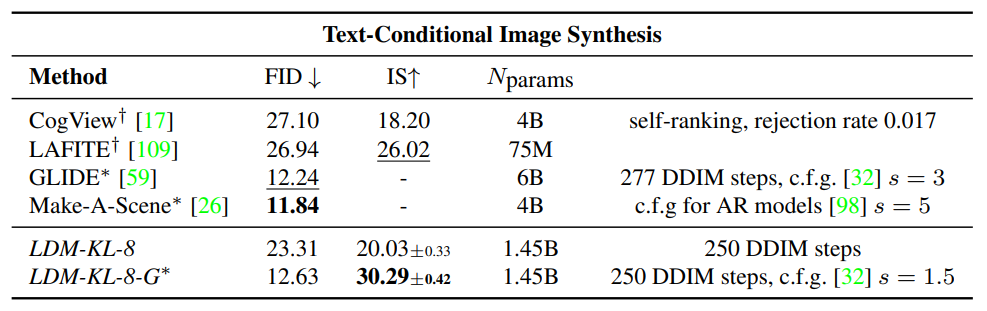
\includegraphics[width=0.6\textwidth]{images/diffusion_models/stable_diffusion/experiments_2.png}
    \caption{Evaluation of text-conditioned image synthesis on MS-COCO dataset. LDM with 250-DDIM steps is on par with the most recent diffusion and autoregressive methods, \textbf{while using significantly less parameters} (1.45 billion) \cite{stable_diffusion}.}
\end{figure}

For text-to-image tasks, the researchers trained a 1.45B parameters model conditioned on language prompts on LAION-400M dataset. The model uses \textbf{BERT-Tokenizer} \footnote{Its important to note that the researchers used the BERT text tokenizer in the paper, however, in the \href{https://github.com/CompVis/latent-diffusion}{offical released implementation of Stable Diffusion} they used CLIP tokenizer. The reason is that in the Imagen paper \cite{imagen}, the researchers found out that using larger language models had more impact on generated image quality than larger image generation components. This fact is shown in figure \ref{fig:imagen_clip_score_bigger_llm}.} \cite{bert} and implement $\tau_\theta$ (the domain-specific conditional encoder) as a transformer.

\begin{figure}
    \centering
    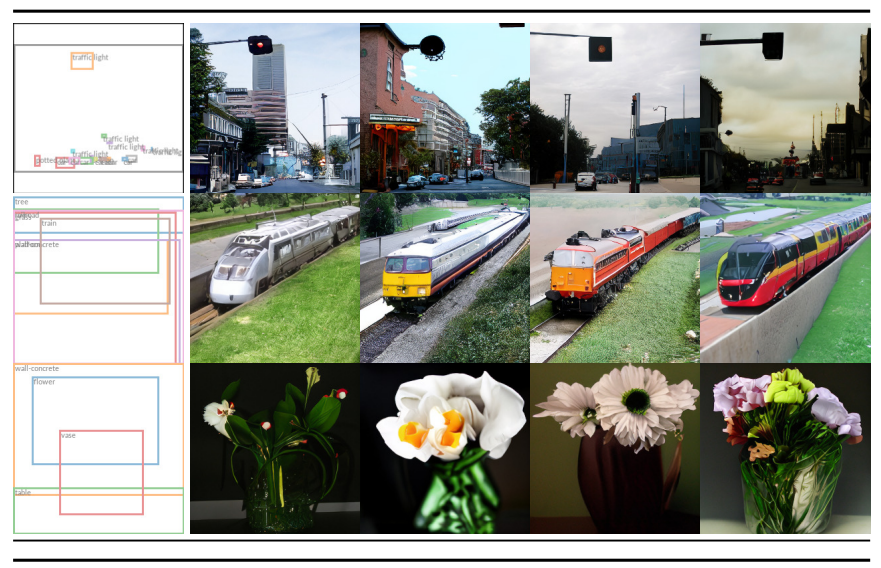
\includegraphics[width=0.5\textwidth]{images/diffusion_models/stable_diffusion/experiments_3.png}
    \caption{Samples of Stable Diffusion conditioned on semantic layouts \cite{stable_diffusion}.}
    \label{fig:stable_diffusion_experiments_semantic_layouts}
\end{figure}

For semantic layouts, the model is trained to synthesis images based on semantic layouts from the OpenImages dataset and fine-tuned on COCO dataset (figure \ref{fig:stable_diffusion_experiments_semantic_layouts}).

In figure \ref{fig:imagen_scaling_encoder_more_impactful_than_unet_scaling}, which is from Imagen paper \cite{imagen}, we see that using larger text encoder has more impact on image quality than larger image generation components (like the U-Net). This is why in Stable Diffusion, the implementation uses CLIP tokenizer instead of BERT tokenizer (which was originally used in the paper).

\section{Imagen}
\label{sec:imagen}

Imagen \cite{imagen} is a T2I diffusion model that builds on the power of large transformer language models \cite{transformer} (LLMs) to generate high-fidelity images. The combination of diffusion and LLMs have shown remarkable outputs. 

The paper has 5 main key takeaways and observations:

\begin{enumerate}
    \item \textbf{Effectiveness of large frozen text encoders}: one of the main observation in the paper that a large frozen language model trained only on text data have a significant impact on the fidelity of generated images compared to increasing the parameters of the diffusion image model. Scaling the language model is easy, since unlabeled text data is abundant and available on the internet.
    \item \textbf{Dynamic thresholding}: is a new sampling technique (section \ref{subsec:imagen_diffusion_guidance_weight}) that improves image fidelity and text-image alignment, which improves upon static thresholding.
    \item \textbf{Effective U-Net}: a new U-Net architecture that is simpler and more memory efficient.
    \item \textbf{COCO FID score of 7.27}: imagen achieved a new state-of-the-art COCO FID score of 7.27, which outperforms all other previous works.
    \item \textbf{DrawBench}: a new human evaluation benchmark for T2I task. Imagen outperforms all other works, including DALL-E \cite{dalle}, VQ-GAN+CLIP \cite{vqgan_clip}, LDM \cite{stable_diffusion}, GLIDE \cite{glide}, and DALL-E 2 \cite{dalle_2}.
\end{enumerate}



















\subsection{Text-to-Text Transfer Transformer (T5)}
\label{subsec:t5}

\textbf{T}ext-\textbf{t}o-\textbf{T}ext \textbf{T}ransfer \textbf{T}ransformer (T5) \cite{t5_model} by Google Research is a language model that treats tasks as a text-to-text (T2T) problems. For example we could prompt the model:

\begin{itemize}
    \item \textbf{Summarization}: "Translate the following text to a summary: ..."
    \item \textbf{Translation}: "Translate the following text from English to French: ..."
    \item \textbf{Text classification}: "Classify the following text into one of the following categories: ..."
    \item \textbf{Question answering}: "Answer the following question: ..."
\end{itemize}

as well as other T2T tasks. In short, this knowledge can be viewed as developing a 'general-purpose' model that can understand text, instead of explicitly training the model to complete the specific downstream task.

The T5 model is open-source and was trained on large corpora of textual data. The base version of the model (T5-base) consists of 220 million parameters, while the largest version of the model (T5-XXL) consists of \textbf{11 billion parameters}. In the context of Imagen, \textbf{the Imagen model uses a frozen version of T5-XXL model} to encode conditional text prompts.

\textbf{Pre-training}: Unsupervised learning is appealing because unlabeled text data is abundant and available on the Internet. For example, the Common Crawl project \cite{common_crawl_project} is a non-profit organization that crawls the internet and provides free access to its achieved datasets to the public. A lot of research has been done on LLM models on large scale datasets, and the consensus is that \textbf{the larger the dataset, the better the model performs} \cite{radford2019language} \cite{jozefowicz2016exploring} \cite{hestness2017deep}. The T5 models were trained on the "Colossal Clean Crawled Corpus" (C4) dataset, which consists of 750GB of English text data scraped from the web.

\textbf{The training objective} of T5 model is called \textbf{span corruption}, which is stronger version of \textbf{masked language modeling}. Given a sentence, some words and some contiguous words are masked (in masked language modeling, only single words are masked), and the model should predict those words. For example: "Thank you for inviting me to your party last week", where the masked words are "for inviting" and "last". And the model should predict those words in the following sentence: "Thank you [MASKED] me to your party [MASKED] week". The model should learn to reconstruct the missing tokens.

\begin{figure}[h]
    \centering
    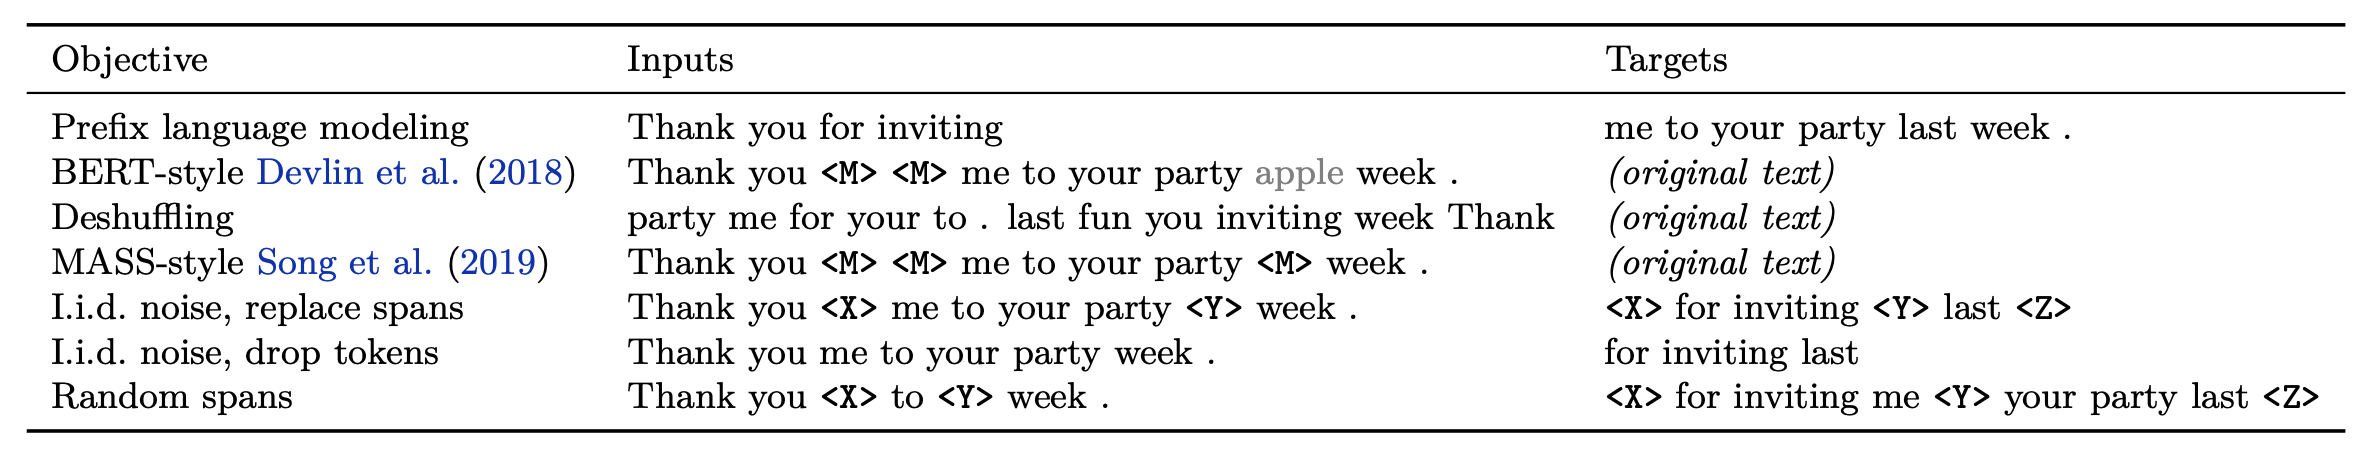
\includegraphics[width=1\textwidth]{images/imagen/t5_objectives.png}
    \caption{Mask modeling in T5 \cite{t5_model}.}
    \label{fig:t5_objectives}
\end{figure}

In figure \ref{fig:t5_objectives} \textless M\textgreater\ denotes shared mask token (the same mask token is used to represent all masked positions in the input). \textless X\textgreater, \textless Y\textgreater, and \textless Z\textgreater\ denote sentinel tokens which have unique token IDs; they mark specific masked positions that the model should reconstruct.















\subsection{Pre-trained text encoders}

In Imagen \cite{imagen} the researchers explored some of the biggest and most advanced text encoders: \textbf{T5-XXL} \cite{t5_model}, \textbf{GPT} \cite{gpt} \cite{mingpt} \cite{gpt_another}, and \textbf{BERT} \cite{bert}. These LLMs were trained exclusively on text datasets, which are substantially larger compared to image-text pair datasets (as used in models like \textbf{CLIP}).

Freezing these models \footnote{When we freeze models we generally mean that some (or all) of the parameters of the model are not changed during training. How? When a layer is frozen during training, no gradient updates will occur for this layer. Gradients will still flow from frozen layer to non-frozen layer, it doesn't skip the backpropagation. It just passes the gradients from the next layer to the previous layer.} provides significant advantage over training them: less memory and compute costs.














\subsection{Diffusion guidance weight}
\label{subsec:imagen_diffusion_guidance_weight}

As described before (section \ref{subsec:classifier_free_diffusion_guidance}), there are two methods to increase sample quality with the tradeoff of diversity:

\begin{itemize}
    \item \textbf{Classifier guidance} uses a separate, pre-trained classifier model to guide the image generation process in diffusion models by adjusting the noise based on how closely the generated image matches a desired condition.
    
    \item \textbf{Classifier-free guidance} (CFG) removes the need for a separate classifier by training the diffusion model itself to optionally condition on the label or text input.
\end{itemize}

More formally, in CFG, sampling is performed weighting the conditional and unconditional signals:

\begin{equation}
    \underbrace{\tilde{\epsilon}_\theta (z_t, c)}_{\text{adj noise prediction}} = \underbrace{w \epsilon_\theta (z_t, c)}_{\text{conditional score}} + \underbrace{(1 - w) \epsilon_\theta (z_t)}_{\text{unconditional score}}
    \label{eq:classifier_free_guidance}
\end{equation}

where $\epsilon_\theta$ is the noise prediction with the learned parameters $\theta$, $w$ is the guidance weight, $c$ is the condition, and $z_t$ is the latent variable at timestep $t$.

Imagen depends on CFG for effective text conditioning. They found that increasing the guidance weight improves image-text alignment but reduces image fidelity. Its caused by \textbf{train-test mismatch}: looking at equation \ref{eq:classifier_free_guidance} if we set $w$ to 1, then we disable CFG, and then the model won't be trained on unconditional samples (only on conditional signals). This causes the model to generate outputs that exceed the noise prediction in the normalized range of [-1, 1]. And when iteratively applying the model to its own outputs at each step, errors caused by this mismatch accumulate, which causes unnatural artifacts in output images. When we set $w>1$ then it improves the model's image-text alignment, but damages image fidelity.

For this reason they investigated static thresholding and dynamic thresholding:

\textbf{Static thresholding} applies the clipping operation to force the $x$-prediction output to fit to the normalized range of [-1, 1]. However, static thresholding still result in over-saturated and less detailed images as the guidance weight approaches 1.

\textbf{Dynamic thresholding}: instead of clipping the $x$-prediction to the normalized range, it sets a dynamic threshold $s$ based on the distribution of absolute pixel values in the current $x$-prediction, allowing the threshold to adapt to the specific output of the model at that moment. In other words, if the pixel values are saturated (close to the [-1, 1] range), dynamic thresholding pushes them inwards by thresholding in the range [-$s$, $s$] and then dividing by $s$.

\begin{figure}
    \centering
    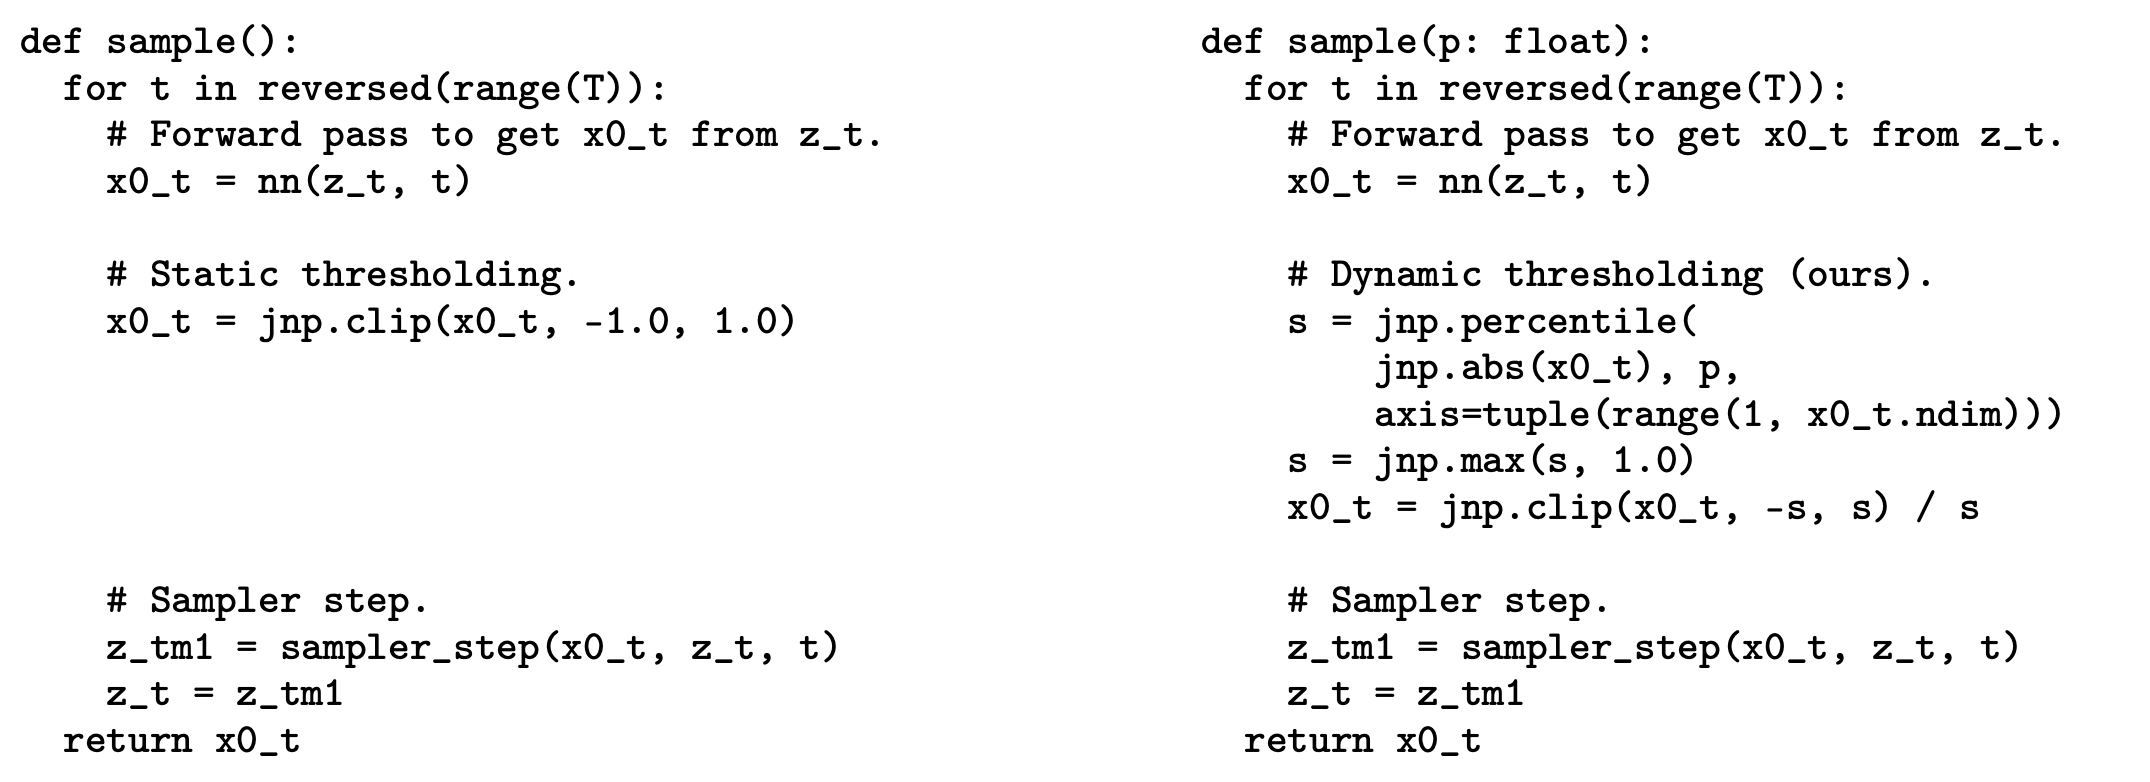
\includegraphics[width=0.7\textwidth]{images/imagen/static_dynamic_thresholding.png}
    \caption{Static (left) and dynamic (right) thresholding code implementation \cite{imagen}.}
    \label{fig:imagen_dynamic_thresholding}
\end{figure}

\begin{figure}
    \centering
    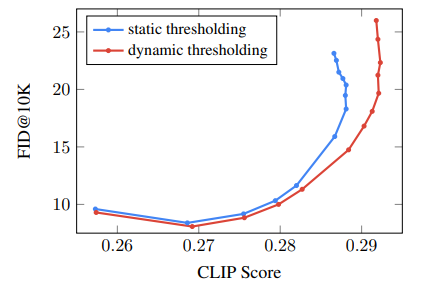
\includegraphics[width=0.4\textwidth]{images/imagen/static_vs_dynamic_thresholding.png}
    \caption{Static vs dynamic thresholding \cite{imagen}.}
    \label{fig:imagen_static_vs_dynamic_thresholding}
\end{figure}

The implementation of static and dynamic thresholding is shown in figure \ref{fig:imagen_dynamic_thresholding}. The impact of dynamic thresholding is shown in figure \ref{fig:imagen_static_vs_dynamic_thresholding} where its shown that dynamic thresholding produces samples with higher image-text alignment (CLIP) and fidelity (FID) compared to static thresholding.
















\subsection{Super-resolution via Repeated Refinement (SR3)}

\label{subsec:imagen_sr3}

In a 2021 paper \cite{sr3}, the Google Research team introduced a new super-resolution model based on diffusion process. \textbf{S}uper-resolution via \textbf{R}epeated \textbf{R}efinment (SR3) model upsamples in iterative manner, similar to reverse diffusion. It upsamples images from $64\times 64$ to $256\times 256$ and finally to $1024\times 1024$.

SR3 achieves close to a 50\% fool rate (47\%) \footnote{A 50\% fool rate means humans can't distinguish between a generated face image and an image of a real face.} on $16\times 16 \rightarrow 128\times 128$ faces, outperforming the previous state-of-the-art GAN models (FSRGAN and PULSE).

\textbf{Iterative refinement}: Given low-resolution image $x_{low}$ the model applies \textbf{bicubic interpolation} \footnote{Bicubic interpolation is a method for resizing images that uses the closest 4x4 pixels grid to estimate new values, resulting in smoother transitions (compared to nearest-neighbor or bilinear interpolation) and fewer visual artifacts.} to upscale the image to the target resolution to get high-resolution image $x$ and then concatenates $x$ with pure Gaussian noise $y_t \sim \mathcal{N} (0, I)$ channel-wise (see figure \ref{fig:sr3_architecture}). Then the U-Net iteratively refines the image $(x, y_t)$ by denoising. The output of a single refinement step (from the U-Net) is $y_{t-1}$. Then in the next refinement step, $x$ is concatenated with $y_{t-1}$ and the process is repeated until we reach $y_0$. The final output is a high-resolution image $y_0$. Note that both $x$ (after the upsampling), $y_i$ are all on same resolution / dimension (see figure \ref{fig:sr3_architecture}).

\textbf{The architecture of SR3} modified the diffusion U-Net: they replaced the original DDPM residual blocks with residual blocks from BigGAN \cite{biggan_deep}, rescaled skip connections by $\frac{1}{\sqrt{2}}$, increased the number of residual blocks, and increased the number of the channel multipliers \footnote{Channel multipliers in a U-Net are the scaling factors used to adjust the number of feature channels at different U-Net layers. In other words, they increased the depth of the features at the cost of decreasing resolution at the convolution layers (down convolution, up convolution layers)} at different resolutions.

% \begin{table}[h!]
%     \centering
%     \begin{tabular}{|l|m{8cm}|}
%         \hline
%         \textbf{Prior to Super Resolution} & \textbf{Limitations} \\ \hline
%         Autoregressive Models           & Computationally expensive; Limited resolution \\ \hline
%         Variational Autoencoder         & Sub-optimal sample quality \\ \hline
%         Generative Adversarial Network  & Difficult to optimize; Requires additional functions to prevent instability \\ \hline
%     \end{tabular}
%     \caption{Related works to super-resolution to SR3 and their limitations compared to SR3.}
% \end{table}


\begin{figure}
    \centering
    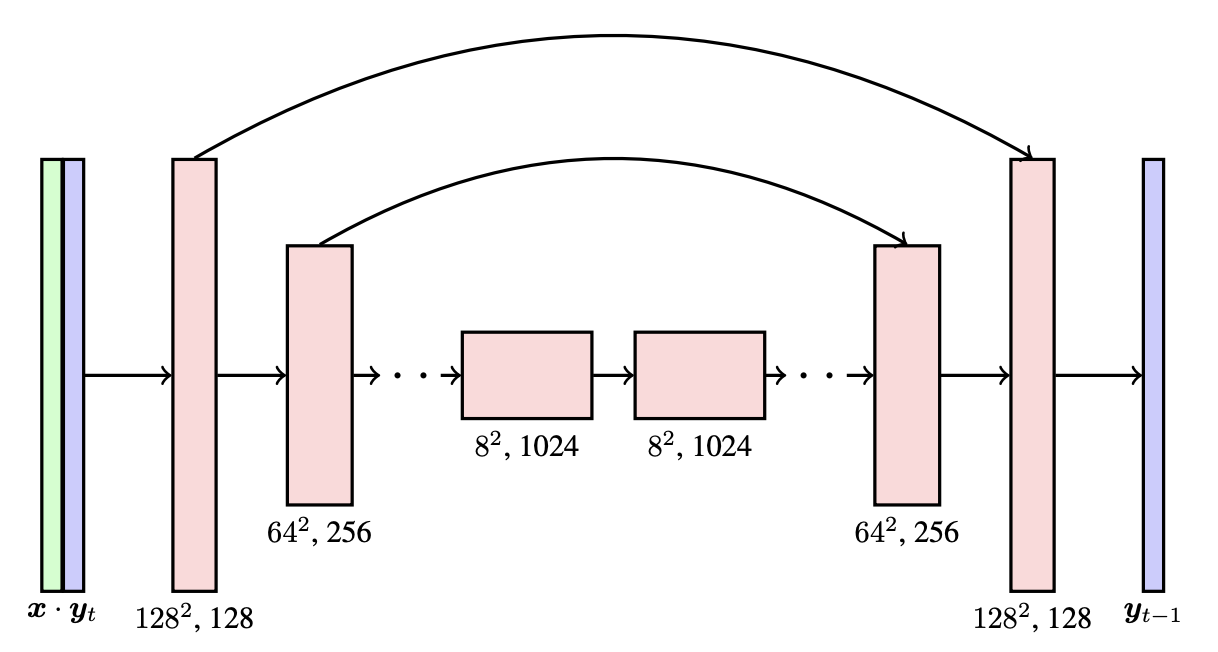
\includegraphics[width=0.5\textwidth]{images/imagen/sr3_architecture.png}
    \caption{SR3 $16\times 16 \rightarrow 128\times 128$ upsampling where $x$ is the input image, upscaled to the target resolution using bicubic interpolation, and then its concatenated with the noise $y$ \cite{sr3}.}
    \label{fig:sr3_architecture}
\end{figure}















\subsection{Cascaded diffusion models (CDMs)}

Cascaded diffusion models, introduced in a 2022 paper \cite{cascaded_diffusion_models} by Google Research, builds upon the SR3 paper \cite{sr3} and introduces a new method for super-resolution (SR) called Cascaded Diffusion Models (CDMs). CDMs use a base diffusion model that output image at low resolution, followed by a sequence (pipeline) of SR3 SR diffusion models that progressively upsamples until we reach the target resolution.

The CDM paper \cite{cascaded_diffusion_models} outperformed VQ-VAE 2 \cite{vqvae2} and BigGAN-deep \cite{biggan_deep} in SR task in FID metric on ImageNet dataset.

A big strength of CDMs is the ability to train and fine tune each model individually.

\textbf{Conditioning augmentation} is the main and critical part of the paper \cite{cascaded_diffusion_models}, which allows to generate images with higher FID, compared to without conditioning augmentation. Conditioning augmentation involves using data augmentation techniques on the low-resolution input image for each SR model in the cascaded pipeline. Augmentations such as Gaussian noise and Gaussian blur are applied to the  to the image which helps prevent each SR model from overfitting to the low-resolution input.

\begin{figure}
    \centering
    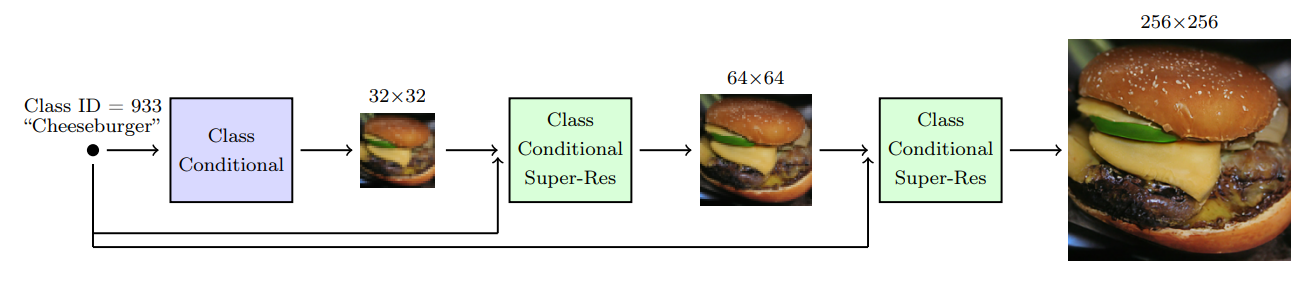
\includegraphics[width=0.7\textwidth]{images/imagen/cdm_architecture.png}
    \caption{CDM upsamples low-resolution image in the pipeline, conditioned on labels \cite{cascaded_diffusion_models}.}
    \label{fig:imagen_cdm_architecture}
\end{figure}























\subsection{Architecture}

An overview of Imagen architecture is shown in figure \ref{fig:imagen_architecture}.

The researchers conducted experiments with frozen LLMs such as BERT \cite{bert}, T5 \cite{t5_model}, and CLIP \cite{openai_clip} and found that humans prefer T5-XXL over CLIP. T5-XXL (T5-Extra Extra Large) text encoder maps text prompts to embeddings. The T5-XXL model has 11 billion parameters, and its the largest version of the T5 model. All the diffusion models are conditioned on the same text embeddings.

\textbf{Base model}: the base model is a $64\times 64$ T2I diffusion model. The network is conditioned on text embeddings (via cross-attention and layer normalization layers), as well as with diffusion timestep embeddings, similar to the class embedding conditioning in the CDM paper \cite{cascaded_diffusion_models}.

\textbf{SR models}: they used modified U-Net based on the improved DDPM paper \cite{openai_improved_ddpm} by OpenAI, By improving the U-Net they achieved 2-3x faster inference and convergence speed; they call this variant "\textbf{Efficient U-Net}". For the $256\times 256 \rightarrow 1024\times 1024$ SR model, they removed self-attention layers but keep the cross-attention layers.

\textbf{Efficient U-Net}: is a new U-Net architectural variant for SR models. Its more memory efficient and \textbf{2-3x faster in training and inference time}. There are several modifications to the U-Net architecture:

\begin{enumerate}
    \item \textbf{More residual blocks}: adding more residual blocks for lower resolutions, since lower-resolution images typically have more channels. They used 8 residual blocks at lower-resolution compared to typical 2-3 residual blocks used in a standard U-Net.
    \item \textbf{Scaling the skip connections} by $\frac{1}{\sqrt{2}}$, similar to SR3 \cite{sr3}, significantly improves convergence speed.
    \item \textbf{Reversing order of downsampling and upsampling blocks}: In a standard U-Net downsampling block, downsampling occurs after the convolution layers, and in the upsampling block, upsampling is done before the convolutions. They reverse this order for both blocks which significantly improves the forward pass without performance degradation.
\end{enumerate}

The efficient U-Net architecture for $64\times 64 \rightarrow 256\times 256$ is shown in figure \ref{fig:imagen_efficient_unet}.

\begin{figure}
    \centering
    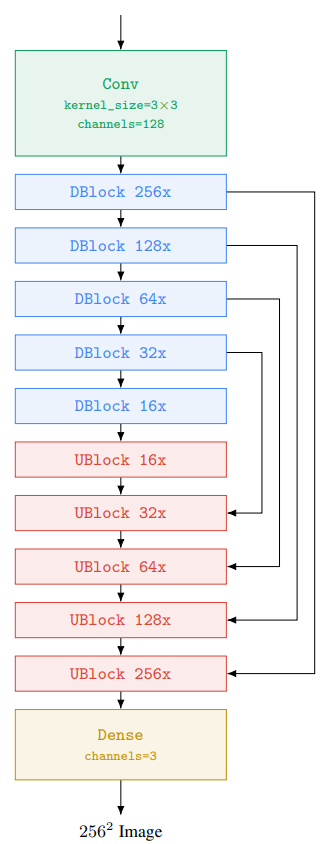
\includegraphics[width=0.25\textwidth]{images/imagen/efficient_unet.png}
    \caption{Efficient U-Net architecture for $64\times 64 \rightarrow 256\times 256$ SR model, proposed in Imagen \cite{imagen}.}
    \label{fig:imagen_efficient_unet}
\end{figure}

Similar to LDMs, Imagen also uses CFG \cite{classifier_free_guidance} (section \ref{subsec:classifier_free_diffusion_guidance}). Imagen depends critically on CFG for effective text conditioning.

\begin{figure}
    \centering
    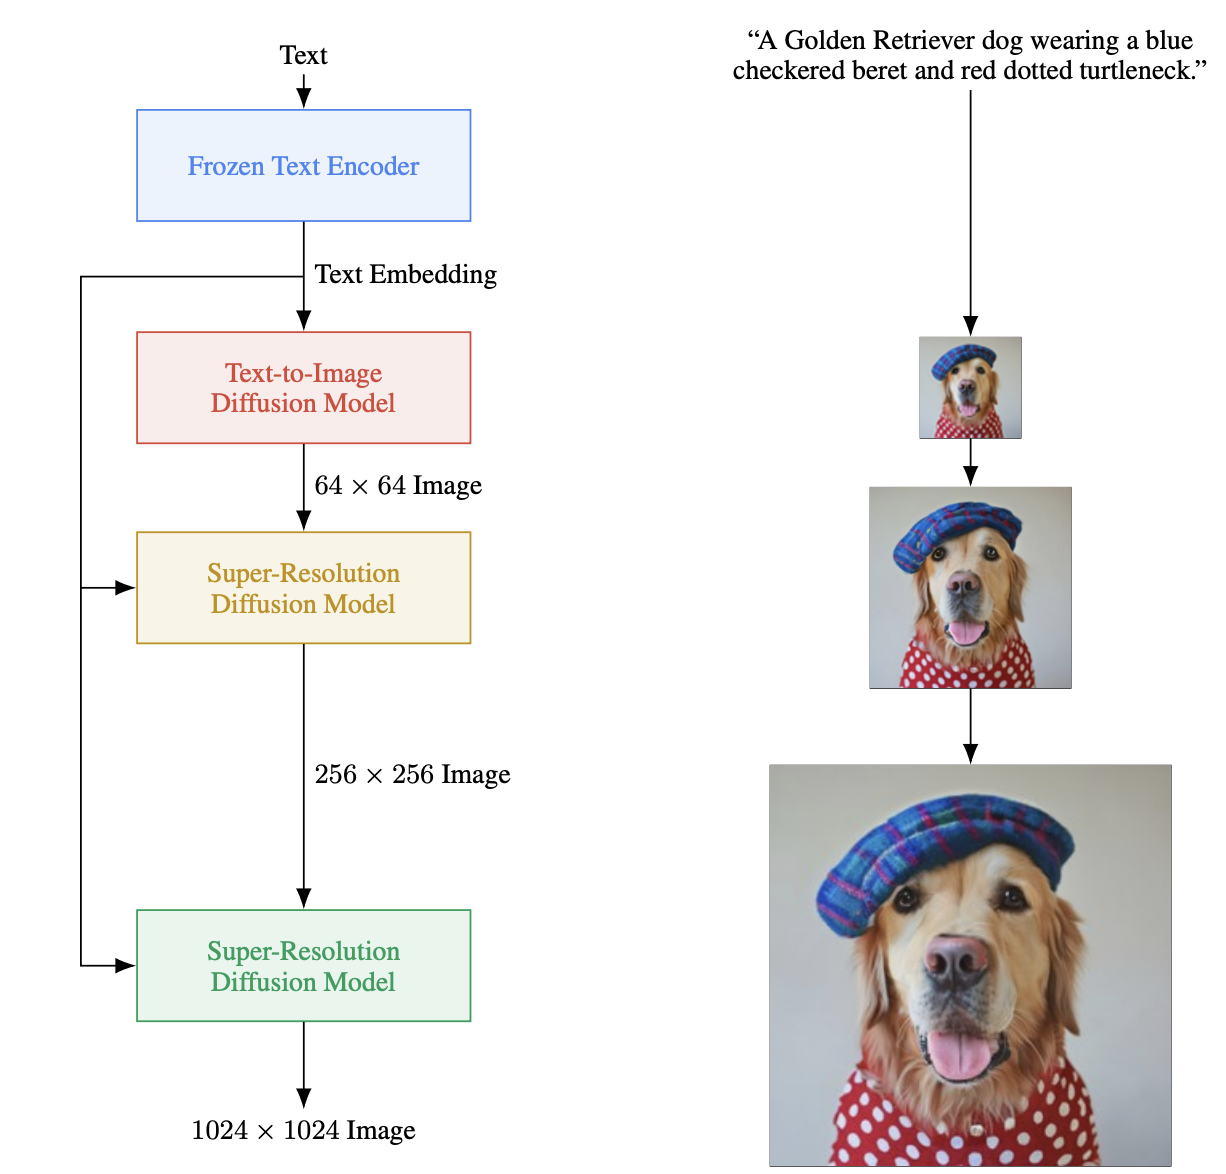
\includegraphics[width=0.5\textwidth]{images/imagen/architecture.png}
    \caption{Overview of Imagen architecture \cite{imagen}.}
    \label{fig:imagen_architecture}
\end{figure}

\textbf{Noise conditioning}: Imagen corrupts the $64\times 64$ image with Gaussian noise. The amount of noise is random at training but arbitrary at inference time. They control the amount of corruption with \textit{aug\_level}, and the SR model is conditioned on the augmentation level.

\textbf{Number of parameters}: the base T2I diffusion $64\times 64$ model has 2 billion parameters. The $64\times 64 \rightarrow 256\times 256$ SR model has 600 million parameters, and the $256\times 256 \rightarrow 1024\times 1024$ SR model has 400 million parameters. The size of the T5-XXL text encoder is 4.6 billion parameters.

\begin{figure}
    \centering
    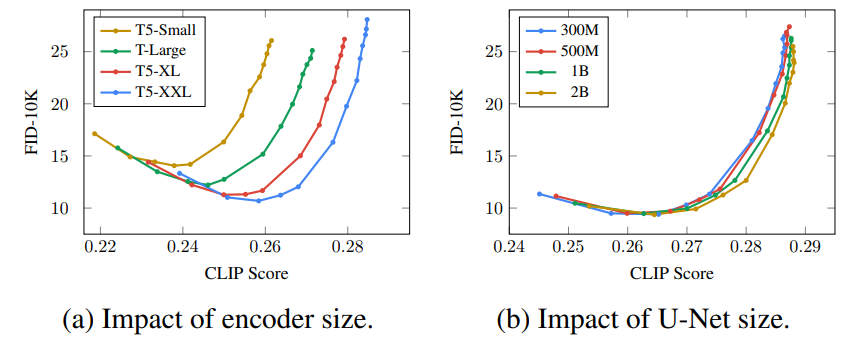
\includegraphics[width=0.75\textwidth]{images/imagen/encoder_vs_unet_size_impact.png}
    \caption{Scaling the encoder size is more impactful than scaling the U-Net size \cite{imagen}.}
    \label{fig:imagen_scaling_encoder_more_impactful_than_unet_scaling}
\end{figure}

\textbf{Scaling text encoder size is more important than U-Net size}: the researchers found that scaling the text encoder has significantly more impact than increasing U-Net size: see figure \ref{fig:imagen_scaling_encoder_more_impactful_than_unet_scaling}.



% DBlock, UBlock

\begin{figure}
    \centering
    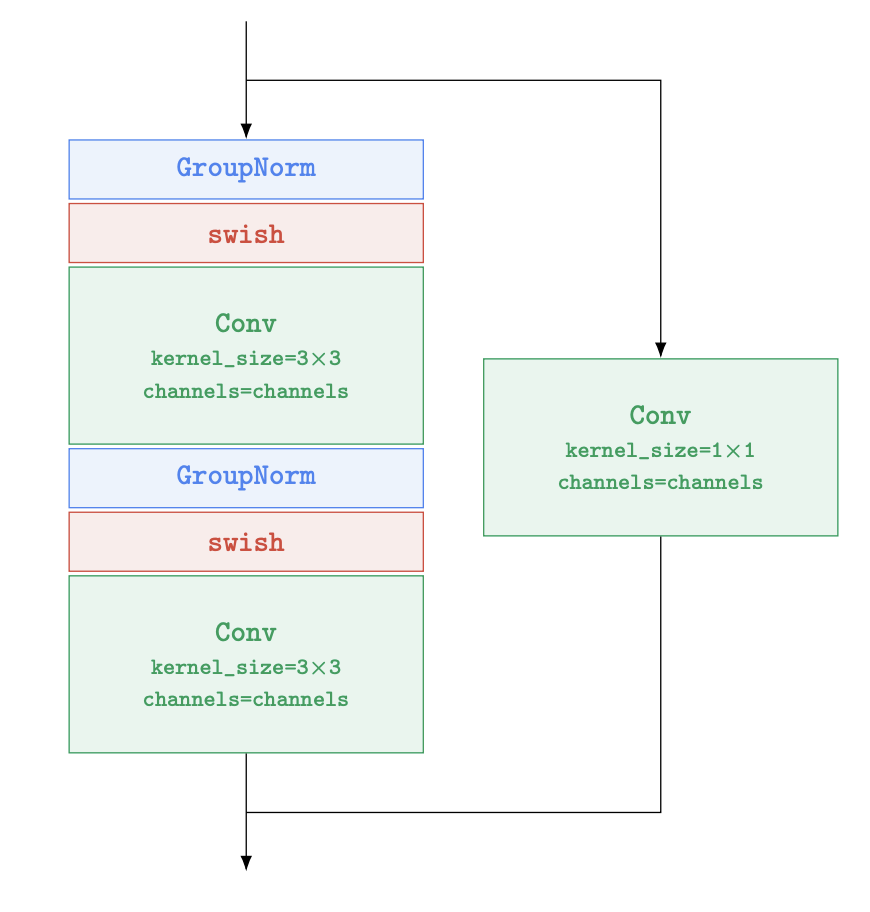
\includegraphics[width=0.35\textwidth]{images/appendix/imagen/unet_resnetblock.png}
    \caption{Imagen efficient U-Net \texttt{ResNetBlock} architecture \cite{imagen}.}
    \label{fig:imagen_resnetblock}
\end{figure}

In figure \ref{fig:imagen_resnetblock} we can see the \texttt{ResNetBlock} which is in use by both the \texttt{DBlock} and the \texttt{UBlock}. The only input of the \texttt{ResNetBlock} is the number of channels. The activation function is Swish (equation \ref{eq:appendix_activations_swish}). 

\begin{figure*}
    \centering
    \begin{subfigure}[b]{0.5\textwidth}   
        \centering 
        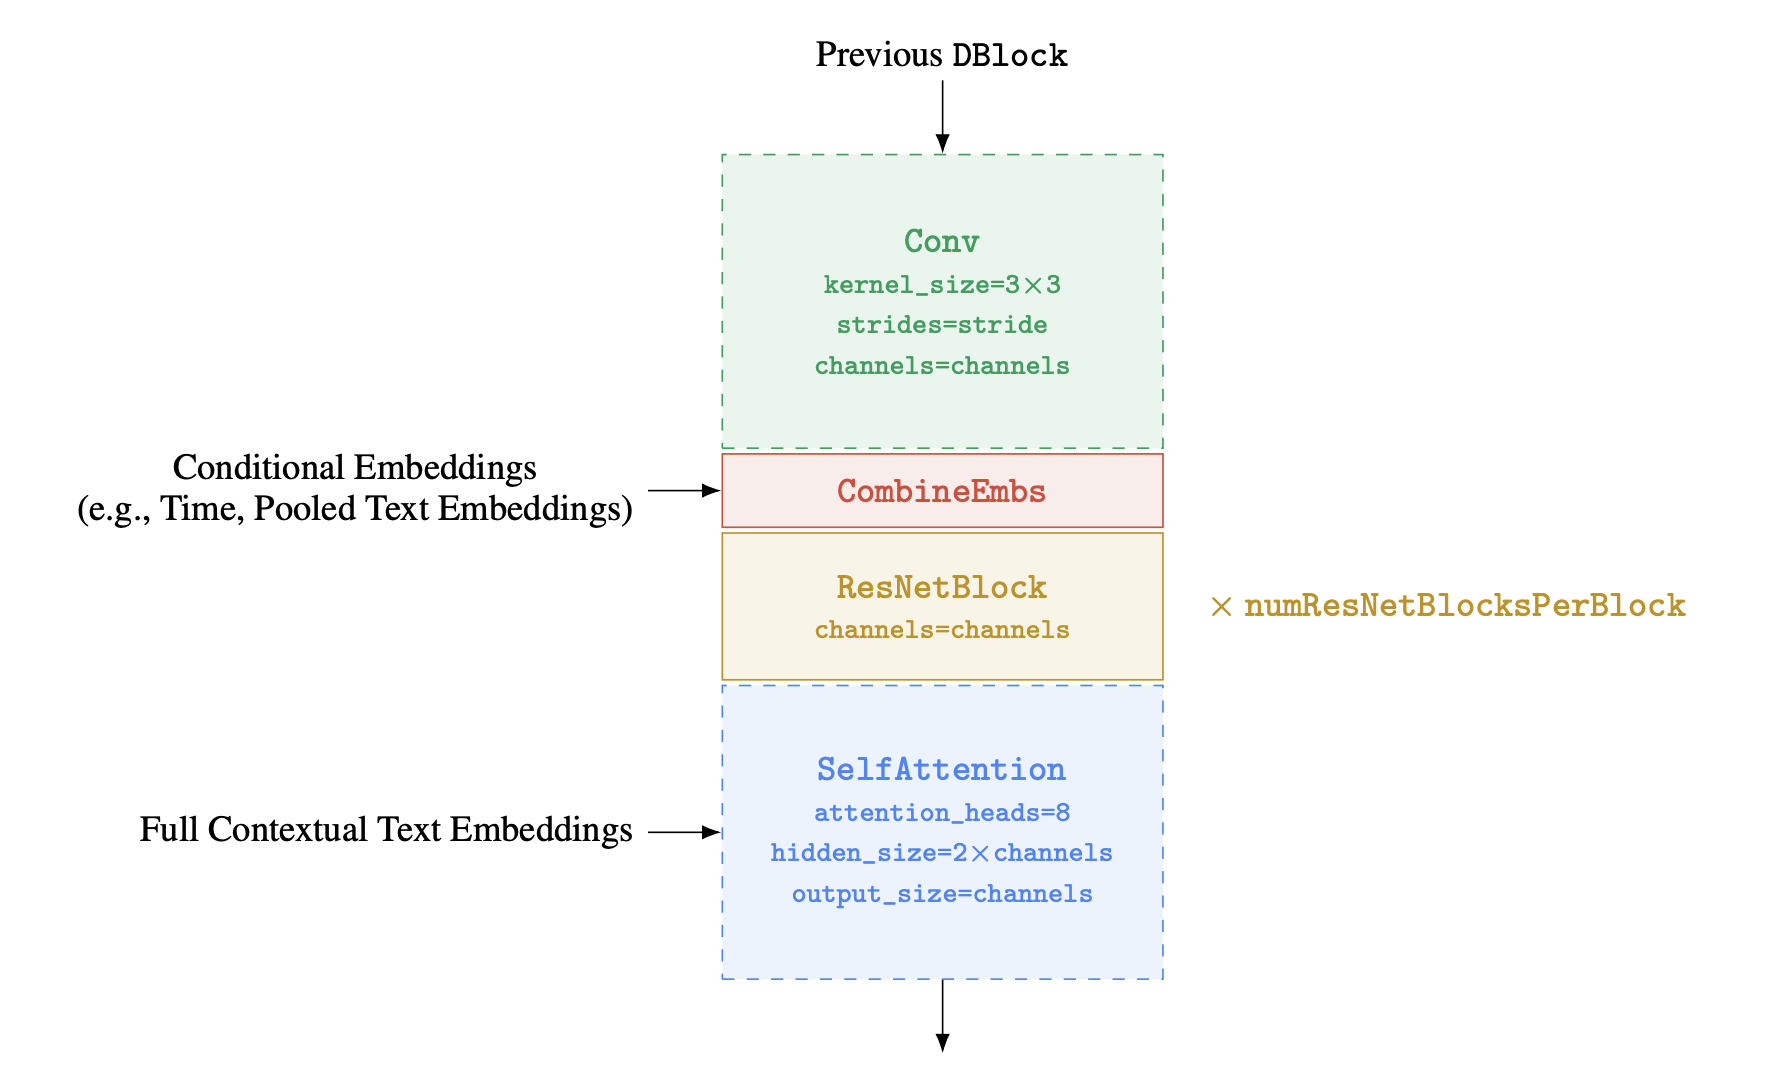
\includegraphics[width=\textwidth]{images/appendix/imagen/dblock.png}
        \caption[]%
        {{\small Imagen efficient U-Net \texttt{DBlock} architecture \cite{imagen}.}}
    \end{subfigure}
    \hfill
    \begin{subfigure}[b]{0.475\textwidth}
        \centering
        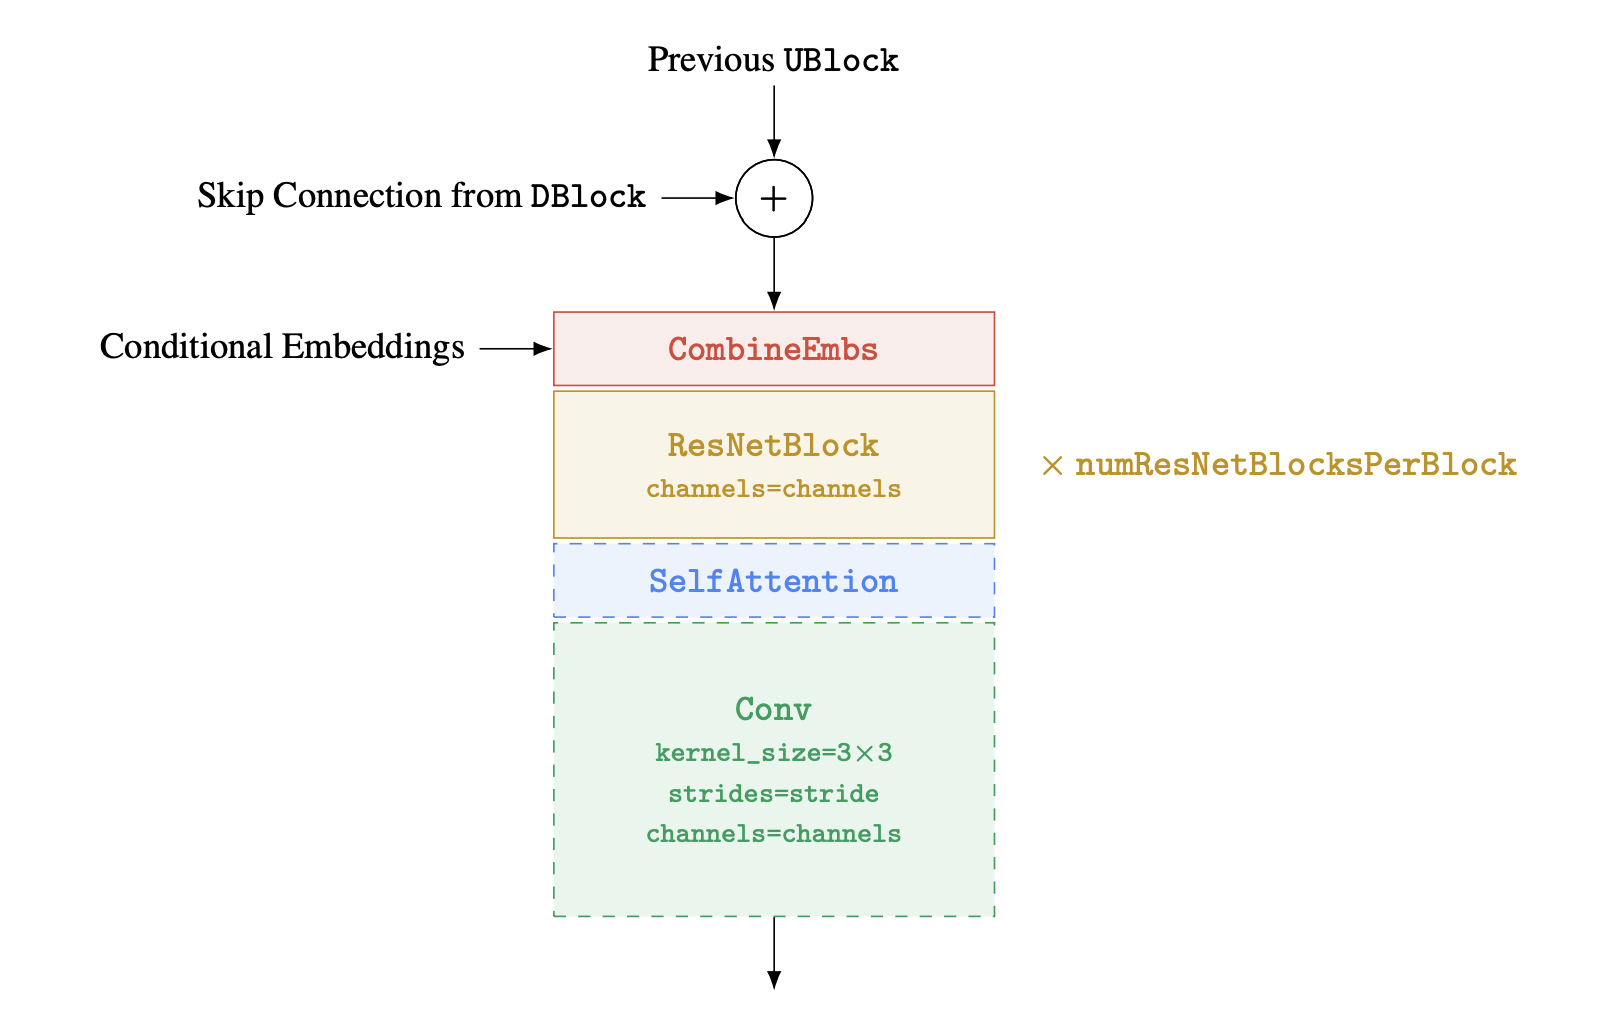
\includegraphics[width=\textwidth]{images/appendix/imagen/ublock.png}
        \caption[]%
        {{\small Imagen efficient U-Net \texttt{UBlock} architecture \cite{imagen}.}}
    \end{subfigure}
\end{figure*}















\subsection{DrawBench}

The COCO dataset \cite{coco_dataset} is a standard benchmark for evaluating T2I models. The standard performance metrics used are FID \cite{fid_score} which measure image fidelity (but is not fully aligned with perceptual quality \cite{perceptual_quality}), and CLIP score \cite{openai_clip} which measures image-text alignment (but is bad at counting objects in an image).

Due to these limitations, the researchers created new benchmark called \textbf{DrawBench} that uses human evaluation to assess image quality by asking the question "Which image is more photorealistic (looks more real)?" and text-image alignment by asking the question "Does the caption accurately describe the above image?". For both cases they used 200 randomly chosen image-caption pairs from COCO dataset.

\begin{figure}
    \centering
    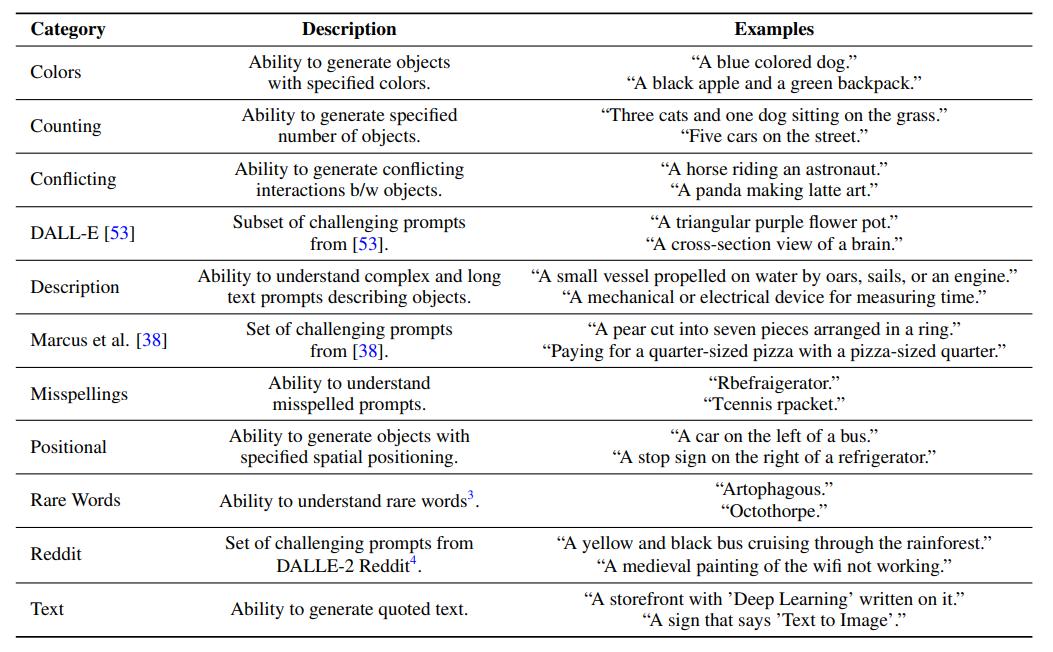
\includegraphics[width=0.6\textwidth]{images/imagen/drawbench_categories.png}
    \caption{Descriptions and examples of the 11 categories in DrawBench \cite{imagen}.}
    \label{fig:imagen_drawbench_categories}
\end{figure}

DrawBench has 11 categories of prompts which test different capabilities of models such as ability to render different colors, number of objects, spatial relations, text in the scene, and more. The prompts include long captions, rare words, and misspelled prompts. See figure \ref{fig:imagen_drawbench_categories} for examples of the categories and examples.














\subsection{Results}

\begin{figure}[t!]
    \centering
    \begin{subfigure}{0.4\textwidth}
        \centering
        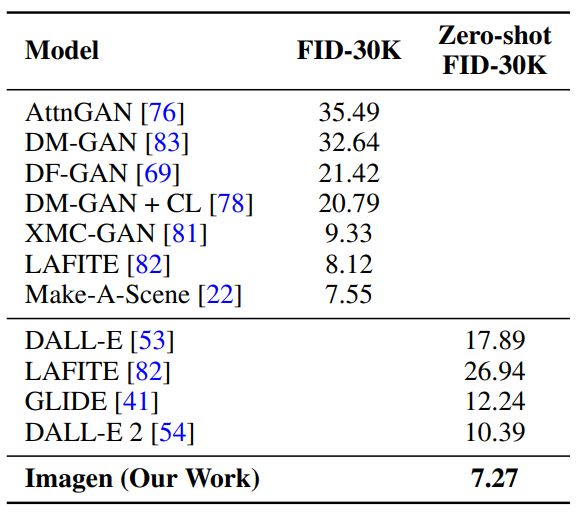
\includegraphics[width=0.6\linewidth]{images/imagen/imagen_coco_zeroshot.png}
        \caption{Although Imagen was not explicitly trained on MS-COCO dataset, it outperforms all other models on COCO FID score, achieving 7.27 FID.}
        \label{fig:imagen_coco_zeroshot}
    \end{subfigure}
    \begin{subfigure}{0.4\textwidth}
        \centering
        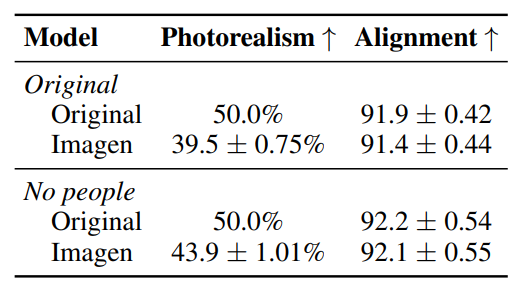
\includegraphics[width=0.6\linewidth]{images/imagen/imagen_coco_human_eval.png}
        \caption{Human evaluation on 256x256 COCO. Imagen splits to two categories: no filters, and human filters. Imagen struggles a little bit with photorealistic people.}
        \label{fig:imagen_coco_human_eval}
    \end{subfigure}
    \caption{Results of Imagen on COCO dataset \cite{imagen}.}
\end{figure}

\begin{figure}
    \centering
    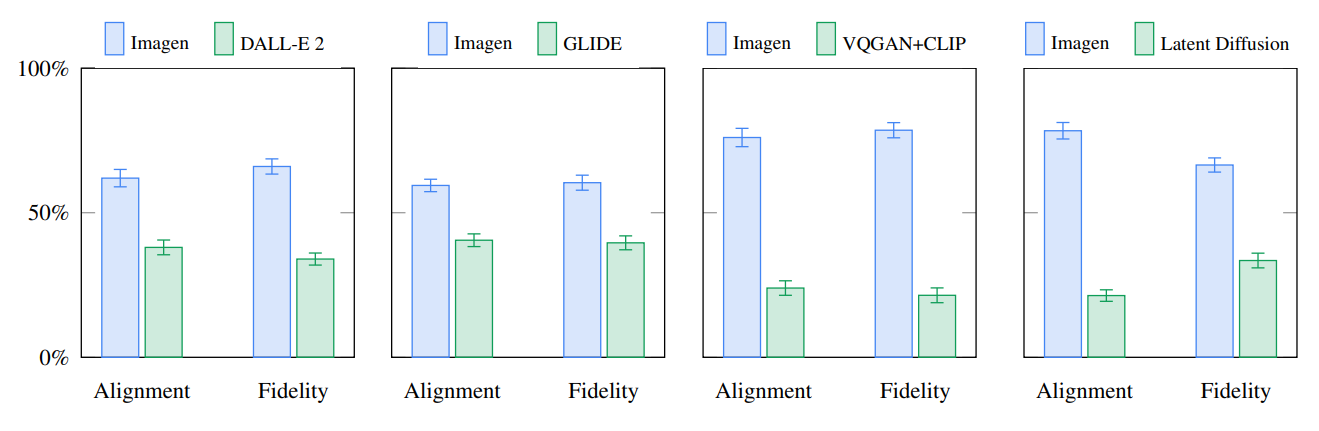
\includegraphics[width=0.6\textwidth]{images/imagen/alignment_fidelity_imagen_vs_models.png}
    \caption{Imagen beats all other models (DALL-E 2 \cite{dalle_2}, GLIDE \cite{glide}, VQGAN+CLIP \cite{vqgan_clip} and Latent Diffusion (Stable Diffusion) \cite{stable_diffusion} (section \ref{sec:stable_diffusion})) in terms of image-text alignment and image fidelity \cite{imagen}.}
    \label{fig:imagen_alignment_fidelity_vs_other_models}
\end{figure}

In figure \ref{fig:imagen_coco_zeroshot} we can see that although Imagen was not trained on the MS-COCO dataset, it still outperforms state-of-the-art models such as DALL-E 2 \cite{dalle_2} and achieves the best MS-COCO FID score of 7.27 in zero-shot setting.

In figure \ref{fig:imagen_coco_human_eval} we can see that Imagen achieves a respectable 43.9\% fool rate on $256\times 256$ COCO human faces, indicating limited ability of Imagen to generate photorealistic people.

In figure \ref{fig:imagen_alignment_fidelity_vs_other_models} we can see that Imagen outperforms all other state-of-the-art models in terms of image fidelity and text-image alignment.


% References / bibliography
\newpage
\printbibliography[heading=bibintoc]{}

% Appendix
\newpage
\section{Appendix}


\subsection{Latent Variables}
\label{appendix:latent_variables}
Latent variables represent the underlying constructs that we can't directly measure. They are denoted by $z$. In the sampling process, we assume a specific probability distribution for $z$ denoted as $P(z)$. This distribution reflects prior knowledge about the latent variable. Usually its the normal distribution (Gaussian):

\[ P(z) = \mathcal{N} (\mu, \Sigma) \]

where $\mu$ is the mean, $\Sigma$ is the covariance of $z$ and $P(z)$ is called the \textbf{prior distribution}. This represents our belief about the distribution of the latent variables before considering the observed data. It helps us incorporate prior knowledge into the model.

Once the observed data ($x$) are collected, the goal is to estimate the \textbf{posterior distribution} of the latent variables, denoted by $P(z|x)$.  This distribution reflects our updated belief about the latent variables after considering the observed data.  Bayes' theorem provides the framework for obtaining the posterior distribution:

\[ P(z|x) = \frac{P(x|z) \cdot P(z)}{P(x)} \]

where $P(x|z)$ is the likelihood function, representing the conditional probability of observing $x$ given a specific value of $z$.


\begin{equation*}
  \left.\begin{aligned}
  z \sim P(z)\\
  x \sim P(x|z)
\end{aligned}\right\} P(x,z) = P(x|z) \cdot P(z)
\end{equation*}


Let's take a real-life example. We know that humans have high intelligence, but we don't have direct measurement for intelligence. IQ tests however, imperfectly measure (estimates) some part of our intelligence. We say that the observable variable is the IQ score, since we can directly and perfectly measure it, and the latent variable is the intelligence. One can describe such relationship with a simple graph:


\begin{center}
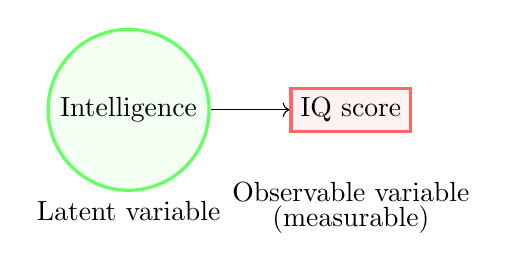
\begin{tikzpicture}[
  roundnode/.style={circle, draw=green!60, fill=green!5, very thick, minimum size=7mm},
  squarednode/.style={rectangle, draw=red!60, fill=red!5, very thick, minimum size=5mm},
]

% Nodes
\node[squarednode] (maintopic) {IQ score};
\node[roundnode] (intelligence) [left=of maintopic] {Intelligence};

% Text labels with positioning
\node [below=of intelligence, yshift=10mm] {Latent variable};
\node [below=of maintopic, yshift=5mm] {Observable variable};
\node [below=of maintopic, yshift=2mm] {(measurable)};

% Lines
\draw[->] (intelligence.east) -- (maintopic.west);

\end{tikzpicture}
\end{center}

This is why we must first measure or observe values $x$ (IQ score), so we can estimate $P(z|x)$ (intelligence). We know that the IQ score tests is Gaussian (normal) distributed with mean ($\mu$) of 100 with standard deviation ($\sigma$) of 15 points. We can say that $P(intelligence)$ is the prior distribution, because it represents our initial belief of possible values of intelligence. If we have little to no prior knowledge about intelligence, we can also assume its uniform distributed, similarly to IQ score.

The posterior distribution $P(intelligence|IQ)$ is the updated belief about the possible values of intelligence \textbf{after} we observed their IQ score. It takes into account the prior knowledge and the information from observed variables, such as IQ.


\subsection{Likelihood function}
\label{appendix:likelihood_function}

Likelihood function in the realm of generative models, is often used to capture the underlying data distribution (generate data points with similar likelihood to the training data distribution).

The formal notion of likelihood function is: $L(x | \theta)$, which reflects the probability of a specific data point ($x$) being generated by the model with its current parameters ($\theta$). We want to maximize this term: $\underset{\theta}{\arg\max}\ L(x | \theta)$. In many cases it's computationally more convenient to maximize the \textbf{log-likelihood} function instead, as the logarithm is a monotonic function (always increasing or decreasing, and therefor the log of the function is also monotonic):

\[
    \hat{\theta}_{MLE} = \underset{\theta}{\arg\max} \ \log L(\mathbf{x} | \theta)
\]

Since directly calculating the likelihood is often intractable, methods like \textbf{maximum likelihood estimation (MLE)} optimize $\theta$ indirectly. To address intractability, approaches such as \textbf{Evidence Lower Bound (ELBO)} are used as alternative loss functions. Additionally, adversarial training is widely employed in GAN-based models.

\subsection{Variational Inference (VI)}
\label{appendix:variational_inference}

Variational inference (VI) is a technique used to approximate complex posterior distributions in Bayesian inference. Instead of directly maximizing the log-likelihood function, VI aims to minimize the \textbf{Kullback-Leibler (KL) divergence} between an approximate posterior distribution and the true posterior distribution (for instance, learn the distribution of 2D points that are generated by the model, which is estimation of another distribution we want the model to learn, for instance, Gaussian). This is often achieved by minimizing a proxy loss function, such as the \textbf{Evidence Lower Bound (ELBO)}, which is tractable (can be effectively computed) to optimize. By minimizing the ELBO, VI effectively guides the approximate posterior distribution towards the true posterior distribution.
\subsection{Kullback-Leibler (KL) divergence}
\label{appendix:kl_divergence}

\begin{figure}
    \centering
    \caption{Showcase of KL-Divergence of three different normal distributions. The divergence between two normal distributions can occur in both mean and variance. Mean (or expectation) is the center of the distribution, while variance is the spread of the distribution.}
    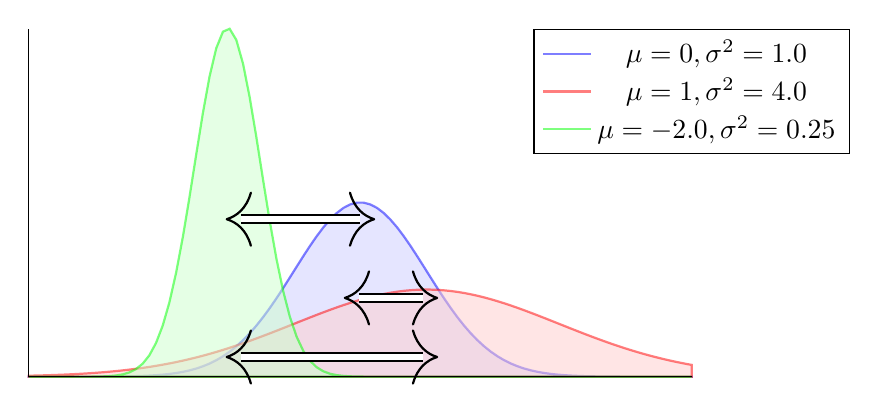
\begin{tikzpicture}
        \begin{axis} [
          no markers, 
          domain=-5:5, 
          samples=100,
          axis lines*=left, 
          height=6cm, 
          width=10cm,
          xtick=\empty, 
          ytick=\empty,
          enlargelimits=false, 
          clip=false, 
          axis on top,
          grid = major,
          legend style={at={(1,1)}, anchor=north, legend columns=1},
        ]

        % Define variables (mean, variance)
        \pgfmathsetmacro{\muA}{0}
        \pgfmathsetmacro{\sigmaA}{1}
        \pgfmathsetmacro{\varA}{\sigmaA^2}
        
        \pgfmathsetmacro{\muB}{1}
        \pgfmathsetmacro{\sigmaB}{2}
        \pgfmathsetmacro{\varB}{\sigmaB^2}
        
        \pgfmathsetmacro{\muC}{-2}
        \pgfmathsetmacro{\sigmaC}{0.5}
        \pgfmathsetmacro{\varC}{\sigmaC^2}
    
        % Blue
        \addplot[blue, thick, fill=blue!20, opacity=0.5] 
        {1/sqrt(2*pi*\sigmaA^2) * exp(-0.5 * ((x-\muA)/\sigmaA)^2)} \closedcycle;
        \addlegendentry{$\mu = \muA, \sigma^2 = \varA$};

        % Red
        \addplot[red, thick, fill=red!20, opacity=0.5] 
        {1/sqrt(2*pi*\sigmaB^2) * exp(-0.5 * ((x-\muB)/\sigmaB)^2)} \closedcycle;
        \addlegendentry{$\mu = \muB, \sigma^2 = \varB$};

        % Green
        \addplot[green, thick, fill=green!20, opacity=0.5] 
        {1/sqrt(2*pi*\sigmaC^2) * exp(-0.5 * ((x-\muC)/\sigmaC)^2)} \closedcycle;
        \addlegendentry{$\mu = \muC, \sigma^2 = \varC$};
        
        \end{axis}

        % Arrows between distributions
        % Blue, Green
        \draw[{<._[sep=-4pt]}-{_[sep=-4pt].>}, line width=0.8pt, double, double distance=2pt] (2.5,2) -- (4.4,2);
        % Green, Red
        \draw[{<._[sep=-4pt]}-{_[sep=-4pt].>}, line width=0.8pt, double, double distance=2pt] (2.5,0.25) -- (5.2,0.25);
        % Blue, Red
        \draw[{<._[sep=-4pt]}-{_[sep=-4pt].>}, line width=0.8pt, double, double distance=2pt] (4,1) -- (5.2,1);

    \end{tikzpicture}
    \label{fig:kl_divergence}
\end{figure}

Kullback-Leibler (KL) divergence allows us to measure the difference between two probability distributions, $P$ and $Q$. It essentially quantifies how much information is lost when using distribution $Q$ to approximate distribution $P$.

In various applications, we deal with situations where we have a true underlying distribution (P) representing the actual data generation process, but we might not know its exact form. We might have another distribution (Q), perhaps a model we've built, that we want to use to represent or approximate the true distribution. KL divergence helps us understand how well Q captures the information present in P. In other words, \textbf{how much diverged the distribution Q is from the distribution P}. See figure \ref{fig:kl_divergence} for a visual representation.

The mathematical formula for KL-divergence is:

\begin{equation}
\label{eq:kl-divergence}
    D_{KL}(P || Q) = \sum_{x \in X} P(x) \cdot log(\frac{P(x)}{Q(x)})
\end{equation}

where $x \in X$ represents all the possible values within the data space ($X$).

A KL-divergence value of 0 indicate that the distribution $Q$ perfectly captures the distribution $P$, and larger numbers indicate higher disparity.

KL-divergence measures information lost, so if both $P,Q$ are Gaussian distributions with the same mean and standard deviation, we have no information lost. But if the standard deviation or the mean is different, KL-divergence measures that. On the other hand, directly integrating the distributions and measuring the area under the curve (AUC) will not show information loss if the standard deviation is the same, but the mean is different.


Other notations are used as well: $p_\theta(x_i), q_\phi(x_i)$. Most of the time we are dealing with small numbers in the probabilities, which will get multiplied with other small numbers, which may result in rounding to zero. So instead we generally compute \textbf{log-likelihood}: $log\ p_\theta(x_i), log\ q_\phi(x_i)$. Now to compare two distributions we can compute the difference: $log\ p_\theta(x_i) - log\ q_\phi(x_i)$ and if that subtraction result in zero that means that our approximated distribution $q$ is identical to ground truth $p$. We can rewrite it like so: 

\begin{equation}
\label{eq:log-likelihood}
    log\ [\frac{p_\theta(x_i)}{q_\phi(x_i)}]
\end{equation}

which is also sometimes called \textbf{log-likelihood ratio}.

In reality, we are only interested in the \textbf{average difference} between $p_\theta$ and $q_\phi$. Because we are dealing with random variables $x \in X$, instead of average we say \textbf{expected value} of a random variable. Weighted average of instances of random variables is:

\begin{equation*}
    \mathbb{E}_{p_\theta} [X] = \sum_{i=1}^{\infty} x_i p_\theta(x_i)
\end{equation*}

where $x_i$ is the state of the random variable, and $p_\theta(x_i)$ is the weight (weight of contribution to the average). A more general formulation is given by:

\begin{equation*}
    \mathbb{E}_{p_\theta} [h(X)] = \sum_{i=1}^{\infty} h(x_i) p_\theta(x_i)
\end{equation*}

where $h(X), h(x_i)$ is a function of random variable $x_i \in X$. This formulation works for discrete random variable, here is the formulation for continuous random variable:

\begin{equation*}
    \mathbb{E}_{p_\theta} [h(X)] = \int_{\mathbb{R}} h(x) p_\theta(x) dx
\end{equation*}

Let's get back to the average likelihood (equation \ref{eq:log-likelihood}), we can set $h(X) = log\ [\frac{p_\theta(x_i)}{q_\phi(x_i)}]$, and we get:

\begin{equation*}
    \sum_{i=1}^{\infty} p_\theta(x_i) log\ [\frac{p_\theta(x_i)}{q_\phi(x_i)}]
\end{equation*}

where $p_\theta(x_i)$ is the weight. This equation is called the \textbf{KL-divergence}:

\begin{equation}
\label{eq:kl_divergence}
    \mathbb{E}_p [log\ \frac{p_\theta(x_i)}{q_\phi(x_i)}]
    =
    \sum_{i=1}^{\infty} p_\theta(x_i) log\ [\frac{p_\theta(x_i)}{q_\phi(x_i)}]
    =
    D_{KL} (p_\theta || q_\phi)
\end{equation}

In short, this is the expected value of the log-likelihood ratio (of discrete random variable). For continuous random variable we get similar formula:

\begin{equation}
\label{eq:kl_divergence_continous}
    \mathbb{E}_p [log\ \frac{p_\theta(x_i)}{q_\phi(x_i)}]
    =
    \int_{\mathbb{R}} p_\theta(x) log\ [\frac{p_\theta(x)}{q_\phi(x)}] dx
    =
    D_{KL} (p_\theta || q_\phi)
\end{equation}

One problem we are dealing with is the infinity space in both equations.  To get around it, we can use the \textbf{law of large numbers} which says:

\begin{equation*}
    \frac{1}{N} \sum_{i=1}^N h(x_i) \approx \mathbb{E}_p [h(X)]
\end{equation*}

and we get:

\begin{equation}
    D_{KL} (p_\theta || q_\phi) \approx
    \frac{1}{N} \sum_{i=1}^N log\ [\frac{p_\theta(x_i)}{q_\phi(x_i)}]
\end{equation}

Credit to \cite{dk-divergence-math-explanation} for the math explanation.
\subsection{Evidence Lower Bound (ELBO)}
\label{appendix:elbo}

Evidence Lower Bound (ELBO) provides an efficient way to optimize and train models that are based on variational inference (often called latent models), like VAEs or GANs. ELBO is an estimation for the log-likelihood function, and since the likelihood function is intractable in latent models (that use latent variables $z$) to calculate directly, ELBO is used instead as approximation (its tractable). ELBO achieves this by setting a lower bound on the likelihood of observing data $x$. By maximizing ELBO we essentially optimize the model by maximizing likelihood.

As we saw in equation \ref{eq:vae_posterior} the likelihood function we want to optimize is:

\begin{equation}
    p(x) = \int p(x | z) \cdot p(z) dz
\end{equation}

where $p(x)$ is the likelihood of observing data $x$, $p(x | z)$ is probability of reconstructing $x$ given latent variable $z$,  $p(z)$ is the prior distribution of latent variable $z$, and the integral is over all possible values of $z$ (if $z$ is discrete, the integral is replaced by a sum).

The reason this integral is intractable is because it is computationally expensive to calculate the likelihood of all possible values of $z$. To solve this, we can use ELBO (also defined at equation \ref{eq:vae_elbo}), which is defined as:

\begin{equation}
    \text{ELBO} = \mathbb{E}_z[\log p(x | z)] - KL(q(z) \Vert p(z))
    \label{eq:elbo}
\end{equation}

where $\mathbb{E}_z[\log p(x | z)]$ is the expected reconstruction loss, and $KL(q(z) \Vert p(z))$ is the Kullback-Leibler divergence (see appendix \ref{appendix:kl_divergence}) between the approximate posterior $q(z)$ and the prior distribution $p(z)$.

The reason this is tractable is because we use mean (expectation) instead of integrating, and both the reconstruction loss and KL divergence are well defined and tractable. 

\subsection{VQ-VAE}

In listing \ref{lst:vq_codebook} we can see that the researchers divided the code vectors by number of embeddings, which normalizes the vectors in order to stabilize the training (the codebook vectors will have unit variance).

\begin{lstlisting}[language=Python, label=lst:vq_codebook, caption=Code of the quantisizer module of VQ-VAE paper. Shows the initialization of the codebook vectors.]
    class VectorQuantizer(nn.Module):
    """
    Discretization bottleneck part of the VQ-VAE.

    Inputs:
    - n_e : number of embeddings
    - e_dim : dimension of embedding
    - beta : commitment cost used in loss term, beta * ||z_e(x)-sg[e]||^2
    """

    def __init__(self, n_e, e_dim, beta):
        super(VectorQuantizer, self).__init__()
        self.n_e = n_e
        self.e_dim = e_dim
        self.beta = beta

        self.embedding = nn.Embedding(self.n_e, self.e_dim)
        self.embedding.weight.data.uniform_(-1.0 / self.n_e, 1.0 / self.n_e)
\end{lstlisting}




\begin{lstlisting}[language=Python, label=lst:vqvae_distance, caption=Euclidean distance calculation in VQ-VAE paper between embedding and codebook vectors $\Vert z-e \Vert$.]

    def forward(self, z):
        """
        Inputs the output of the encoder network z and maps it to a discrete 
        one-hot vector that is the index of the closest embedding vector e_j

        z (continuous) -> z_q (discrete)

        z.shape = (batch, channel, height, width)

        quantization pipeline:

            1. get encoder input (B,C,H,W)
            2. flatten input to (B*H*W,C)

        """
        # reshape z -> (batch, height, width, channel) and flatten
        z = z.permute(0, 2, 3, 1).contiguous()
        z_flattened = z.view(-1, self.e_dim)
        # distances from z to embeddings e_j (z - e)^2 = z^2 + e^2 - 2 e * z

        d = torch.sum(z_flattened ** 2, dim=1, keepdim=True) + \
            torch.sum(self.embedding.weight**2, dim=1) - 2 * \
            torch.matmul(z_flattened, self.embedding.weight.t())
    
\end{lstlisting}


\begin{lstlisting}[language=Python, label=lst:vqvae_loss, caption=Loss function as defined in the VQ-VAE paper (eq. \ref{eq:vq_loss}). The detach keyword is the stop gradient operation.]
    # compute loss for embedding
    loss = torch.mean((z_q.detach()-z)**2) + self.beta * \
        torch.mean((z_q - z.detach()) ** 2)
\end{lstlisting}



\begin{lstlisting}[language=Python, label=lst:vqvae_stop_gradients, caption=Allow gradients to flow through the snapping operation.]
    # preserve gradients
    z_q = z + (z_q - z).detach()
\end{lstlisting}
\subsection{Transformers}
\label{appendix:transformers}

...

\end{document}